\documentclass{article}
\usepackage[utf8]{inputenc}
\usepackage[margin=1in]{geometry}
\usepackage{amsmath}
\usepackage{amsthm}
% Package for making turing machine diagrams %
\usepackage{tikz}
\usetikzlibrary{chains,fit,shapes}
% Packages for algorithms %
\usepackage{algorithm}
\usepackage{algorithmic}
% Package which has the nice looking empty set symbol (\varnothing)
\usepackage{amssymb}
% Package with the ceiling function
%\usepackage{mathtools}
%\DeclarePairedDelimiter{\ceil}{\lceil}{\rceil}
\usepackage{braket}
\usepackage{amsmath} 
\usepackage{amsfonts}
\usepackage{amssymb}
\usepackage{comment}
\usepackage{mathtools}
\DeclarePairedDelimiter{\ceil}{\lceil}{\rceil}
\usepackage{bm}

\usepackage{biblatex}
\addbibresource{library.bib}

% Makes table of contents links clickable in pdf readers
\usepackage[colorlinks=true, linkcolor=blue, urlcolor=blue, citecolor=blue]{hyperref}

% recursive subtraction
\makeatletter
\newcommand{\prc}{\mathbin{\mathpalette\prc@inner\relax}}
\newcommand{\prc@inner}[2]{%
  \vbox{\offinterlineskip\m@th
    \ialign{%
      ##\cr
      \hidewidth\raisebox{-1.5\height}[0pt][0pt]{$#1.$}\hidewidth\cr
      $#1-$\cr
    }%
  }%
}
\makeatother

\theoremstyle{definition}
\newtheorem{definition}{Definition}[section]
\newtheorem{problem}{Problem}
\newtheorem{thesis}{The Church-Turing Thesis}

\theoremstyle{plain}
\newtheorem{example}{Example}[section]
\newtheorem{exercise}{Exercise}[section]

\theoremstyle{theorem}
\newtheorem{fact}{Fact}[section]
\newtheorem{lemma}{Lemma}[section]
\newtheorem{theorem}{Theorem}[section]
\newtheorem{corollary}{Corollary}[section]
\newtheorem{claim}{Claim}[section]

% TO DO
% UTM construction
% Nondeterministic Time Hierarchy Theorem (ugh)
% Cook Levin Proof
% Alternating Machine, ATIME and ASPACE classes
% Circuit model, P/poly, Karp Lipton
% AM/MA, BPP, bounding within PH, Graph Isomorphism likely NP-intermediate
% P sharp, Toda
% IP = PSPACE, MIP = NEXP
% BQP
% Generic complete problems for a class, syntactic vs semantic classes

\title{Computability Notes}
\author{Alex Creiner}
\date{}

\sloppy
\begin{document}

\maketitle

\tableofcontents

% \part{Models of Computation}
There are many different models of computation, and the notion 'a model of computation' is itself vague and only mostly rigorously defined. The closest we can get to a rigorous definition would be to call it a subset of functions which take finite strings as input and return finite strings as output, which meet some criteria. The criteria will involve a lot of words and symbols, but semantically will always boil down to just saying "$f$ is computable if it can be implemented within the model." 

The central model we are concerned about is the Turing machine model, since it lends itself best to the study of the "natural" computational resources - time and space. For the study of computation itself though, we will turn to the recursive functions. The recursive functions could certainly be called a computational model, since basically anything can, but they are conspicuous because there is no 'machine' to be found anywhere in the definition. They are simply a set of functions defined in a very conventional mathy way, via some simple inductive rules. The amazing fact about computation is that every model of computation ever devised has proven to be equivalent to the recursion 'model' in the sense that they end up defining the exact same set of functions. Establishing this connection between Turing machines and the recursive functions rigorously is the central aim of this section. Doing so carefully will prove fruitful in ways far beyond the mission statement, however.

\section{Turing Machines}
In the notes that follow, some symbols should always be taken to refer to specific things unless otherwise noted:

$\Sigma$ will denote an \textbf{alphabet}. That is, a finite set of symbols. 
$\Sigma^*$ will denote the set of finite \textbf{strings} of characters in the alphabet $\Sigma$. Formally, a string is a function $x: \{1,2,3,\ldots,n\}\to \Sigma$ for some $n \leq \omega$. ($\omega$ is how I represent the cardinality of the natural numbers, i.e. $|\mathbb{N}| = \omega$. I'm too lazy to write aleph all of the time.)

\begin{definition}
A \textbf{decision problem} (otherwise known as a \textbf{language}) is a subset $L \subseteq \Sigma^*$.
\end{definition}

Informally, a decision problem is a problem where the answer is yes or no, depending on some input. In the interest of viewing problems as mathematical objects to be studied and categorized, we view these as sets, in particular the set of inputs for which the answer is yes. As an example, consider the following problem:

\begin{problem}
FACTORING: Given an integer $n \in \mathbb{Z}$, does n have a nontrivial factor?
\end{problem}

We will usually define problems informally, like this. Implicitly though, the alphabet is $\Sigma = \{0,1,2,3,4,5,6,7,8,9\}$, and

\[FACTORING = \{n\in\mathbb{Z}: \textrm{n has a nontrivial prime factor}\} \]

A convenient consequence of this formalism is that we can regard all decision problems as questions of set membership. If we are given a set and told that this set is a language, then we can always assume that the decision problem is simply answering the question 'Is $x\in L$?'

\begin{definition}
A \textbf{Turing Machine} is a triple $M=(\Sigma,Q,\delta)$. $\Sigma$ is as above, but in addition to having a blank symbol, we assume that we have an additional \textbf{start} symbol, denoted $\triangleright$. Q is another finite set, called the \textbf{states} of the machine. Q will always be assumed to have three special states - a \textbf{starting state} $q_s$, an \textbf{accepting state} $q_y$, and a \textbf{rejecting state} $q_n$. The states $q_y$ and $q_n$ will be known as \textbf{halting states}. Finally, $\delta: \Sigma \times Q \to \Sigma \times Q \times \{-1,0,1\}$ is known as the \textbf{transition function} of the machine. 
\end{definition}
The transition function explains how the machines behavior. We will explain the semantics more formally shortly, but intuitively, picture a single infinite row of a piece of graph paper (typically referred to as \textit{tape}). At any moment in time, we are 'pointed' at a single cell of the tape, which will have a single symbol $\sigma$ printed on it, and we are in some state, q. 
\vspace{1cm}
\begin{center}
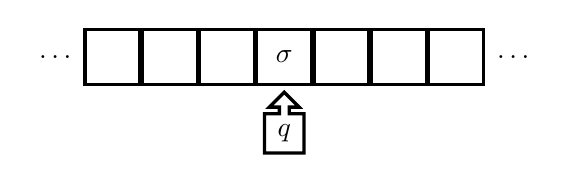
\begin{tikzpicture}
\tikzstyle{every path}=[very thick]
\edef\sizetape{0.7cm}
\tikzstyle{tmtape}=[draw,minimum size=\sizetape]
\tikzstyle{tmhead}=[arrow box,draw,minimum size=.5cm,arrow box
arrows={north: .25cm}]
\begin{scope}[start chain=1 going right,node distance=-0.15mm]
 \node [on chain=1,tmtape,draw=none] {$\ldots$};
 \node [on chain=1,tmtape] {};
 \node [on chain=1,tmtape] {};
 \node [on chain=1,tmtape] {};
 \node [on chain=1,tmtape] (input) {$\sigma$};
 \node [on chain=1,tmtape] {};
 \node [on chain=1,tmtape] {};
 \node [on chain=1,tmtape] {};
 \node [on chain=1,tmtape,draw=none] {$\ldots$};
 \node [tmhead,yshift=-.6cm] at (input.south) (head) {$q$};
\end{scope}
\end{tikzpicture}
\end{center}

The transition function $\delta$ describes what the machine should do in this moment. If 
\[\delta(\sigma,q)=(\lambda,r,d)\]
Then the interpretation is that the machine erases $\sigma$, prints $\lambda$ in it's place, changes to state $r$, and moves the cursor either one cell to the right, one cell to the left, or stays still, depending on whether $d$ is 1,0, or -1 respectively. If $d=1$, then the intuitive picture in the next 'moment' would look like this:
\vspace{1cm}
\begin{center}
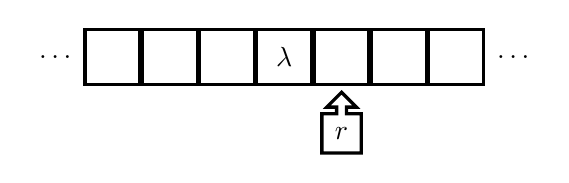
\begin{tikzpicture}
\tikzstyle{every path}=[very thick]
\edef\sizetape{0.7cm}
\tikzstyle{tmtape}=[draw,minimum size=\sizetape]
\tikzstyle{tmhead}=[arrow box,draw,minimum size=.5cm,arrow box
arrows={north: .25cm}]
\begin{scope}[start chain=1 going right,node distance=-0.15mm]
 \node [on chain=1,tmtape,draw=none] {$\ldots$};
 \node [on chain=1,tmtape] {};
 \node [on chain=1,tmtape] {};
 \node [on chain=1,tmtape] {};
 \node [on chain=1,tmtape] (input) {$\lambda$};
 \node [on chain=1,tmtape] (input) {};
 \node [on chain=1,tmtape] {};
 \node [on chain=1,tmtape] {};
 \node [on chain=1,tmtape,draw=none] {$\ldots$};
 \node [tmhead,yshift=-.6cm] at (input.south) (head) {$r$};
\end{scope}
\end{tikzpicture}
\end{center}
We now formalize the semantics of a Turing Machine. The key to this is the notion of a configuration.
\begin{definition}
A \textbf{configuration} of a Turing Machine M is a triplet $c=(T,q,z)$ where $T\in\Sigma^*$, $q\in Q$, and $z\in\mathbb{Z}$.  
\end{definition}
Intuitively, a configuration is a complete description of the state of a Turing Machine at any moment in `time'. The element T is called a \textbf{tape configuration}, and it documents what is printed on the tape, and where. It's important to note that the tape configuration is finite. To understand this, know that a bit further down we will have an initial tape configuration which is always finite, and the machine will always be at some finite number of steps from it's initial state. Thus there will always be a finite string such that everything to the right and to the left is nothing but 'blanks'. This region may shrink or expand, but it is always finite, and we can regard it as the portion of the tape which is 'in use'. This finite used region of tape is the tape configuration $T$. The state is self explanatory, and the natural number $z$ represents the current position of the cursor. There is an implicit assumption in declaring $z$ a natural number, as opposed to an integer. Since $z$ is nonnegative, this means that the tape only extends infinitely in \textit{one direction}. We will show later that this is nothing more than convention - allowing the tape of a Turing machine to be two-way adds nothing profound in the way of what is computationally possible or efficient. For any $n\in\mathbb{N}$, we let $T[n]$ denote the contents of the tape at position n.
\begin{definition}
Let $M=(\Sigma,Q,\delta)$ be a Turing Machine, and $c_1=(T_1,q_1,z_1)$, $c_2=(T_2,q_2,z_2)$ be configurations of M. We say that \textbf{$c_1$ yields $c_2$ in one step} and write $c_1 \overset{M}{\to} c_2$, if $\delta(T_1[z_1],q_1)=(T_2[z+d],q_2,d)$ and $z_2=z_1+d$. Inductively we can extend this definition in the obvious way to define what it means for $c_1$ to yield $c_2$ in k steps for any $k\in\mathbb{N}$, and we use $c_1 \overset{M^k}{\to} c_2$ to denote this.
\end{definition}
Thus we have a formal framework for describing 'steps' of a computation. Towards beginning the machine on some input, let $x\in(\Sigma-\{\sqcup\})^*$. We will call strings like this (that is, finite strings without any blanks), \textbf{inputs}, and we'll allow denote the \textbf{empty string} $\epsilon$ to also be an input. (Often we will refer to inputs as members of $\Sigma^*$, but this is an abuse of notation.) By $|x|$, we mean the \textbf{length} of x (that is, the number of characters in x). By $T_x$, we mean the tape configuration consisting of a single $\triangleright$, followed by $x$. Formally, $T_x[0]=\triangleright$, and $T_x[n]=x_{n-1}$ for $1\leq n \leq |x|+1$. 
\begin{definition}
We say that a Turing Machine M \textbf{halts in k steps} on an input $x\in\Sigma^*$, if for some tape configuration T, some cursor position z, and one of the two halting states $q_h \in \{q_y,q_n\}$, we have that $(T_x,q_0,0) \overset{M^k}{\to} (T,q_h,z)$. If the halting state is $q_y$, then we say that M \textbf{accepts} the input x, and if the halting state is $q_n$, then we say that M \textbf{rejects} the input x. We call the final tape congiguration the \textbf{output} of M, and write $M(x)=T$. If the machine never halts for any number of steps, then we write $M(x)=\nearrow$. 
\end{definition}
Before proceeding further we should come out and be upfront about some incoming hypocrisy regarding the so-called start symbol $\triangleright$. For a two sided infinite Turing machine, which is what we've defined as our standard, the $\triangleright$ only exists for our convenience. The more primal and fundamental form of the model we've described should be understood to make do without it, by having initial configurations begin with the first character of the input string rather than with a $\triangleright$. I have it in my definition because I found it helpful when I was being introduced to theory, and indeed it is sometimes very useful to have a symbol like this.

On the other hand, the blank symbol $\sqcup$ is absolutely fundamentally necessary, and in fact, it should be noted that this symbol has a very special role in the operation of any Turing machine, as it is the \textit{only} symbol which is ever allowed to occur infinitely often on the tape.

Now that we have a formal notion of what it machine to accept or reject an input, we can define what it means for a machine to truly solve a problem for us.
\begin{definition}
Let L be a language, and M be a Turing Machine. We say that M \textbf{decides} L if for all inputs $x\in\Sigma^\#$,
\[x\in L \Rightarrow \textrm{M accepts x in k steps for some k} \]
\[x \notin L \Rightarrow \textrm{M rejects x in k steps for some k}\]
\end{definition}
Note that we can't get away with simply writing the first condition with an $\iff$ and have an equivalent definition, since the machine may \textit{neither} accept \textit{nor} reject an input. The machine may simply trail on forever, never reaching a conclusion.
\begin{definition}
    If a language/decision problem $L$ is decidable by a Turing machine, we say that the language is \textbf{recursive}. Alternatively, we say that it is \textbf{decidable}, or \textbf{computable}. We call the set of all recursive languages \textbf{R}.
\end{definition}
Before moving on, we extend our definition of Turing machines to machines which are allowed multiple tape 'strings'. This extension is equivalent to the original model in it's capabilities, and takes the idea of a Turing machine from something abstract and foreign to one which will, with a bit of practice, quickly feel startlingly natural.
\begin{definition}
A \textbf{k-string Turing machine} is a triple $M=(\Sigma,Q,\delta)$, with $\Sigma$ and Q just as before. The only thing that is different is the transition function. Now, $\delta: \Sigma^k \times Q \to \Sigma^k \times Q \times \{-1,0,1\}^k$.
\end{definition}
The interpretation is that we now have multiple strings of tape, and multiple cursors positions to keep track of. At any single step, we are reading k symbols, and we are allowed to alter all of them in a single step before moving the k cursors left or right independently of each other. Configurations are just as before, except not we need k integers to keep track of cursor positions, and k strings of tape. Thus, the configurations of a k-string Turing machine are (2k+1)-tuples
\[c=(T_1,T_2,T_3,...,T_k,q,z_1,z_2,z_3,...,z_k) \]

We would still like for our inputs and outputs to be single strings, rather than vectors, so we take as the output only the contents of the last string of the machine, and record inputs on the first. Thus, for an input string $x\in \Sigma^\#$, our initial configuration would look like
\[c_x=(T_x,\epsilon, \epsilon,...,\epsilon,q_0,0,0,0,...,0) \]
Where $\epsilon$ denotes the tape configuration consisting of a $\triangleright$ followed by nothing but blanks. It should be obvious that adding multiple strings would provide a noticable boost in efficiency over single string machines. We will show shortly that this boost is not particularly significant. Before that we need to discuss in a bit more detail the philosophy of what we're actually trying to do here. 

What we are interested in is, in general, analyzing the \textit{difficulty} of computational problem. What \textit{is} difficulty? 

We should first note that in some sense, we talk about difficulty as a quantity. We talk about \textit{how difficult} something is. We say that this problem is \textit{more difficult} than some other problem. This is our initial assumption - difficulty is a quantity.

As a quantity, difficulty is still more complicated than most others. While we haven't proven that they exist yet, it can certainly be said that any problem which isn't computable is more difficult in a sense than any problem which \textit{is} computable. So in some sense, the problems which aren't computable are going to be \textit{infinitely} difficult. And yet, we will see that we are still able to measure and categorize tiers of difficulty nonetheless. It stands to assume then that difficulty as a quantity is more deeply connected to the generalization of the natural numbers known as the ordinal numbers - numbers which proceed past infinity. This ordinal property of difficulty can in some sense be traced to it's fundamental subjectivity. What is difficult in one sense might be easy in another sense. If a problem is impossible for normal computers, it may nonetheless be possible for a computer which has been equipped a certain special additional property. 

We will get to this, but primarily we will be interested in the difficulty of problems which \textit{are} computable, and in this sense we can think of difficulty as a distinct finite number. Even here, difficulty is a \textit{fuzzy concept}. It's presence was known before we even realized that it was a quantity, making it fundamentally different to the quantities that mathematicians and physicists are typically used to dealing with; who's definitions are baked into their method of measurement. For inspiration then, we turn to the social scientists, who are more used to dealing with this sort of thing. 

A psychologist wishes to analyze quantities like difficulty all of the time. They have words like isolation, alienation, greed, dominance - character traits which are clearly quantities and clearly philosophically valid ideas, but which nonetheless exist with no clear 'ruler' for measuring them. Nonetheless, the psychologist or sociologist wants to do controlled experiments just like any other scientist. They want to test hypotheses such as ``The social isolation of individuals increases proportionally to the length of the working day.''

I believe that the social scientists accomplish this by forming an \textit{operational} definition of alienation. What they do is define some material, measurable behaviors which can reasonably be \textit{associated} with social isolation. For example, suppose they decide to track the lives of 30 individuals, 15 of which work 12 hour days, and 15 of which work 8 hour days. For each person in the experiment, the scientist decides to measure, say, the amount of time spent conversing with friends and family outside of work. While this is not a concrete measure of isolation by any means, it can reasonably be argued that the results say something meaningful about isolation in general, and more importantly, \textit{very few would argue that} time spent talking with friends would decrease with isolation. As other social scientists create their own operational definitions for social isolation and conduct similar experiments, the aggregate can prove results through an exhaustive inability to falsify, arguable just as well as a physicist can prove results about their more 'concrete' quantities such as charge and mass. We will define several types of resources for which large amounts could reasonably be seen as signs of high difficulty. 

How can we form an operational definition for the difficulty of a computational problem? The gateway lies in the computational model. Suppose we have a Turing machine which decides a problem for us. Implicit to this model are certain resources which can be monitored. Number of steps, for instance, or amount of 'scratch paper' used. There are many more. Just as 'amount of time spent talking to friends and family' can be used in the negative for 'measuring' social alienation, the \textbf{runtime} of a Turing machine - number of steps which the machine takes to complete it's computation, can be used in the positive to 'measure' the difficulty of a problem. There is here still a complication though. 

Tracking the resource use of a specific computation isn't good enough to measure the difficulty of an entire problem. Problems, as we've defined them, involve infinitely many computations - one for any problem for which the answer is yes or no. 

Since any problem contains an infinite number of possible instances, in order to analyze the feasibility of a problem, we need to look at how resource requirements go up relative to how complicated the instance of the problem is. There is probably no objection to assuming that, as a rule of thumb, the larger the \textit{length} of an input is, the more demanding an instance of the problem becomes. If an input is long, we should expect that deciding if $x\in L$ will be more resource intensive than if the input was short, \textit{regardless} of what resource is being considered.

Thus, to measure the feasibility or difficulty of a problem, we need to define a resource of interest within a particular model of computation (for our purposes, the Turing model), and then track how quickly the use of that resource gets out of hand, as the input length increases. One of the primary advantages of the Turing model is that two resources which feel very natural to think about as scaling with difficulty feel just as natural to track within the model - time and space. We'll begin with time.

\begin{definition}
Let M be a Turing machine which, for some input x, halts after t steps. Then we say that the \textbf{time required by M on input x is t}. We say that \textbf{M operates in time $f(n)$}. if, for any string x, the time required by M on x is at most $f(|x|)$. 
\end{definition}

Note that our definition here implicitly is concerned with `worst-case' performance, in that the function $f$ is characterizes the machine $M$ as an upper bound. If we had replaced the words `at most' with 'at least' we would instead be concerned with `best-case' performance. Best-case, worst-case, and even average-case performance are all worthy of consideration. However, worst-case is the place to begin, and in many senses the most important of the three.

Suppose that $L_1$ and $L_2$ are problems which are computed by Turing machines operating in time $f(n)$, $g(n)$ respectively, and that these are the best known Turing machines which solve the problem. To compare the difficulty of these problems is to compare the \textit{growth rates of these two functions $f$ and $g$}. But now there is some question of how to compare these two functions. For instance, suppose that $g(n) = f(n)+1$. Then it is true that $g(n)$ is always bigger, but is $L_2$ really a more difficult problem than $L_2$? Certainly not. One extra step per computation is meaningless in the grand scheme of things. We would wish in this case to view the problems as $L_2$ and $L_1$ to be in the same general difficulty class. 

The same decision will be made in the case of $g(n) = cf(n)$ for some positive constant $c$. The decision to view problems like this as 'the same' difficulty is more questionable, but in the end just as well justified by the fact that by utilizing a larger alphabet, we can improve the performance of any Turing machine for \textit{arbitrary} amounts of linear speedup. We won't prove it in these notes, but we will state it for the record, and prove what is in some sense the inverse result shortly. (A full proof can be found in Papadimitriou)

\begin{theorem}[The Linear Speedup Theorem]
	Suppose that $L$ is decidable by a Turing machine $M$ which operates in time $f(n)$. Then for any $\epsilon > 0$, there exists a Turing machine $M'$ with a larger alphabet than $M$ which operates in time $\epsilon f(n)+n+2$.
\end{theorem}
Practically any nontrivial problem is going to take more than $n$ steps to solve, since it always takes \textit{at least} $n$ steps to just scan the input. Any machine which operates in time less than $n$ would have to be populated by questions which can be answered without even looking at the input, hence the triviality.

Recall from calculus that two functions $f(n)$ and $g(n)$ are \textbf{comparable} if  the $f(n) = cg(n)$ for some constant $c$ - that is to say, $\lim_{n \to \infty} \frac{f(n)}{g(n)} = c$. It follows from the linear speedup theorem that we should view problems which are solvable by Turing machines operating in comparable amounts of time should be seen as 'the same' difficulty.

Thus, in complexity theory, we are concerned exclusively with \textit{general classes} of growth rates, rather than specifics. To help us talk about things more simply, we define what is known as big $O$ notation, as well as some other things for later.
\begin{definition}[Big O]
Let $f,g:\mathbb{N} \to \mathbb{R}$. We say that \textbf{$f(n) \in O(g(n))$} if there exists a $c \in \mathbb{R}$ such that for all $n \in \mathbb{N}$, we have $f(n) \leq cg(n)$. 
\end{definition}
It's impossible to tell a difference, but that O is supposed to actually be the Greek letter capital omicron.
\begin{definition}[Little o]
	Let $f,g:\mathbb{N} \to \mathbb{R}$. We say that $f(n) \in o(g(n))$ if 
	\[\lim_{n \to \infty}\frac{f(n)}{g(n)} = 0 \]
\end{definition}

Usually we only care about $O$ and $o$ for functions which are positive and nondecreasing, and we will assume this is always the case unless otherwise noted. To point out some differences between these two things, first note that any $g(n)$ is \textit{always} in $O(g(n))$, but \textit{never} in $o(g(n))$. Also note that $o(g(n)) \subseteq O(g(n))$ Think of the difference between $O$ and $o$ as being akin to the difference between $\leq$ and $<$, but for growth rates. If $a < b$, then $a \leq b$, but obviously not the other way around. For big-O, functions in $O(g(n))$ grow \textit{incomparably slow or comparably fast} to $g(n)$. For little-o, functions in $o(g(n))$ grow \textit{incomparably slow}, nothing in $o(g(n))$ is allowed to match $g(n)$ in terms of growth rates.

\begin{definition}[Big $\Omega$]
	Let $f,g: \mathbb{N} \to \mathbb{R}$. We say that $f(n) \in \Omega(g(n))$ if there exists a positive $c \in \mathbb{R}$ such that $f(n) \geq cg(n)$.  
\end{definition} 

$\Omega(f)$ is $O(f)$'s sunny, optimistic, and often neglected sister. The idea is that $g(n) \in \Omega(f(n))$ grow \textit{comparably fast or incomparably faster} than $f$. So we take functions in $O(f)$ to be 'slower or similar' to $f$, and functions in $\Omega(f)$ to be 'faster or similar' to $f$. In this way, $\Omega$ will be useful to discuss \textit{best-case} performance, just as $O$ will be used to discuss worst-case. Discussion of best-case performance in complexity theory would amount to discussion of the \textit{optimality} of an algorithm - a proof that there is nothing better. Proofs of these kinds of claims are hard and rare, and so $\Omega$ tends to significantly less use than her brother. (For the record, the $O$ and $o$ in the notation are technically Greek capital and lowercase omicrom, but this looks identical to a regular o or O in the English alphabet.)

A \textbf{complexity class} is any nonempty proper subset of \textbf{R}. This is \textit{not} going to be a completely rigorous definition. For now though, this will do. We will make this more precise later.
\begin{definition}
	 For any function $f:\mathbb{N} \to \mathbb{R}$, let \textbf{TIME($f(n)$)} denote the class of languages L such that there exists a Turing machine M which decides L, operates in time $g(n)$, for some $g \in O(f)$
\end{definition}
So \textbf{TIME}$(f(n))$ is the set of all decision problems which are decidable by an algorithm which operates in time \textit{less than or equal to} $cf(n)$ for some $c$. Note that $f(n)$ could be $2^n$, and our problem might be solvable by an algorithm which works in linear time, and this language would still be in \textbf{TIME}$(2^n)$. Again this hearkens to the fact that in complexity theory, we are interested primarily (but not exclusively) in \textit{worst-case complexity}. If it's better, that's great, but the concern of the theory revolves around being 'no worse than'. We summarize this formally with a simple fact:
\begin{fact}
	If $f(n) \in O(g(n))$, then \textbf{TIME}$(f(n)) \subseteq \textbf{TIME}(g(n))$ 
\end{fact}
Next we turn to an inspection of the second natural resource associated with the Turing model - space. to start, picture yourself sitting at a desk, performing some long computation. You have a sheet of paper with the input, and a specific sheet to record the output onto, and you are blindly following some set of instructions to produce an output. Two obvious 'resources' should come to mind. One of these resources is the amount of time the computation takes, which we have formally captured above. The other is the amount of \textit{scratch paper} you need. 

Space is an interesting resource, because it has a fascinating inverse relationship with time. To illustrate this, let's consider the basic grade school algorithm we are taught to compute the sum of two numbers. Suppose we want to add the numbers 346 and 89. Our 'scratchwork' would look something like this:
\begin{center}
\begin{tabular}{c@{\,}c@{\,}c@{\,}c}
  & 1 & 1 &   \\
  & 3 & 4 & 6 \\
+ &   & 8 & 9 \\ 
\hline
  & 5 & 3 & 5 \\
\end{tabular}
\end{center}

In considering space complexity, the + sign and the line separating summands from sum are completely unnecessary and shouldn't be considered. Nor should the two numbers we are adding or the final output. (Remember, we are only considering the amount of scratch paper we need, and the input/output is on a separate page). Without these, it would seem like the only extra space needed are for the two carry bits. If we're given two numbers, the bigger of which has length, say, n, then the input can be taken to be of length 2n, and the maximum number of carry bits that we might possibly need is n-1. It would seem like our basic grade school addition algorithm operates in linear space, O(n).

But we don't really \textit{need} n-1 bits of space, do we? Once we use the carry bit and move leftward to the next digit, we won't need the old carry bit anymore. \textit{Provided we don't value our time, we could simply reuse that space}. We could leave the bit as a 1 if we need to carry another bit in the next step, or \textit{erase it} and replace it with a 0 if we don't. Again, \textit{provided we don't care about time constraints}, addition is actually uses only a \textit{single bit} of space!

We will see many more examples of this dynamic at play. To summarize, space as a resource is fundamentally different than time in that it is \textit{reusable}, and therefore, \textit{at the cost of time}, we can \textit{usually} save space. How much space can we save in general? It seems like the answer to this questions should vary wildly depending on the algorithm, so perhaps we should reword the question: What is the \textit{maximum} amount of space that we could \textit{possibly} save? The answer to this question seems to be exponential.  

In order to properly exclude the input and output in considerations of space, we make use of multiple strings. We will append extra strings to be reserved as input and output. We want to make damn sure that nothing worth considering ever happens on these two strings, so we take measures in the next definition to make sure that the input string is \textit{read only}, and the output string is \textit{write only}.
\begin{definition}
A \textbf{k-string Turing machine with input/output} is a k+2-string Turing machine with the condition that if $\delta(\sigma_1,\sigma_2,...,\sigma_{k+2},q)=(\rho_1,\rho_2,...,\rho_{k+2},r,...,d_1,d_2,...,d_k)$, then $\sigma_1 = \rho_1$ and $i_k \neq -1$
\end{definition}

This condition ensures that no symbols of the input string can be overwritten, and that the cursor of the output string can only move forward. 
The definitions for time complexity easily apply to k-string machines with no alterations. We are ready to define the space used in a computation for these types of machines. After doing so we can state a theorem which confirms that there is no loss of generality in viewing any ordinary Turing machine as a Turing machine with input/output, assuring that this definition can be applied generally.
\begin{definition}
Let M be a single string Turing machine with input/output, and suppose that M halts on input $x \in \Sigma^\#-\{\sqcup\}$ after t steps. For $l=0,...,t$, let $c_l = (T_1,...,T_{k+2},q,z_1,...,z_{k+2})$ denote the configuration of M, initially in configuration $c_x$, after l steps. Then the \textbf{space required by M on input x} is the number
\[\max_{l\leq t}\{\sum_{i=2}^{k+1}|T_i|\} \] 
Note that for a Turing machine with only one work string, this amounts to simply the maximum length of that string at any step, i.e. $\max_{l \leq t}(|T_2|)$. For a function $f:\mathbb{N}\to \mathbb{R}$, we say that \textbf{M operates in space $f(n)$} if for any input $x \in \Sigma^*-\{\sqcup\}$, the space required by M on x is at most $f(|x|)$. 
We also define the class $\bm{SPACE}(f(n))$ to be the collection languages L which are decidable by some Turing machine M operating in space $g(n)$, for some $g \in O(f(n))$. Just as we noted above, it is obvious that for any $g(n) \in O(f(n))$, $\bm{SPACE}(g(n)) \subseteq \bm{SPACE}(f(n))$.
\end{definition}
Now is as good a time as any to make an extremely simple but nonetheless important observation, one which would appear deep for computer scientists used to more complicated models of computation, but for Turing machines is clear as day:
\begin{fact}
For any function $f:\mathbb{N} \to \mathbb{R}$, 
\[\textrm{\textbf{TIME}}(f(n)) \subseteq \textrm{\textbf{SPACE}}(f(n)) \]
\end{fact}
\begin{proof}
If L is decided by a k-string Turing machine in $f(n)$ steps, then there is certainly no way to move more than $kf(n) \in O(f(n))$ tape cells in either direction!
\end{proof}
This is as far as we're going to go for now with respect to complexity theory. Before we can talk in detail about this topic, we need to note some basic things about Turing machines. We went to the trouble early on of defining these things because it will be important to analyze resource use as we go through the first wave of basic results, which we turn to now.

Consider the Turing machine $M = (\{\triangleright,\sqcup,0,1\},\{s,h,q,q_0,q_1\},\delta)$, with $s$ the starting state and $h$ a halting state, and $\delta$ defined as follows:
\begin{center}
\begin{tabular}{ |c c|c| } 
 \hline
 State & Symbol & Output of $\delta$ \\ 
 \hline
 $s$ & $0$ & $(s,0,1)$ \\ 
 $s$ & $1$ & $(s,1,1)$ \\ 
 $s$ & $\sqcup$ & $(q,\sqcup,-1)$ \\
 $s$ & $\triangleright$ & $(s,\triangleright,1)$ \\
 $q$ & $0$ & $(q_0,\sqcup,1)$ \\
 $q$ & $1$ & $(q_1,\sqcup,1)$ \\
 $q$ & $\sqcup$ & $(q,\sqcup,0)$ \\
 $q$ & $\triangleright$ & $(h,\triangleright,1)$ \\
 $q_0$ & $0$ & $(s,0,-1)$ \\
 $q_0$ & $1$ & $(s,0,-1)$ \\
 $q_0$ & $\sqcup$ & $(s,0,-1)$ \\
 $q_0$ & $\triangleright$ & $(h,\triangleright,1)$ \\
 $q_1$ & $0$ & $(s,1,-1)$ \\
 $q_1$ & $1$ & $(s,1,-1)$ \\
 $q_1$ & $\sqcup$ & $(s,1,-1)$ \\
 $q_1$ & $\triangleright$ & $(h,\triangleright,1)$ \\
 \hline
\end{tabular}
\end{center}
The reader should show to themselves with a simple example that this machine simple creates a single blank space in between the starting $\triangleright$ and the input $x$, and then halts. That is to say, $M(x) = \sqcup x$. This is a useless program on it's own, but it serves a smaller 'building' block in the sense that it would be nice if we could use this within the context of building something bigger. Perhaps we are designing a Turing machine which at some point needs to create a space somewhere on it's work string. We would detect the need for this of course via finding a particular symbol-state pair, call them $\sigma$ and $v$ respectively. What we could do is define $5$ new states for the machine we are building, corresponding to the $5$ in this machine above and one more, call it $v$, as well as the new 'special' symbol, $\underline{\sigma}$, where $\sigma$ is the symbol for which you want everything to the right of it moved over. For simplicity, we will assume that none of the letters used in the $Q$ above have been used yet. First, we have the command $\delta(\sigma,v) = (\underline{\sigma},s,0)$. From here, everything is defined \textit{exactly} as above. The 'starting state' $s$ now takes the form of an initialization of a subroutine, and the 'halting state' $h$ would take the form of a completion of that subroutine. 

We will need this subroutine shortly for a specific proof, but more generally it points to a principle which we will can make extensive use of going forward:
\begin{center}
	In principle, given we have defined previously a machine which produces a specific function, we can without any extra justification use this machine as a subroutine in the creation of larger programs. 
\end{center}
	By this same principle we also but we also have the following important lemma:
\begin{lemma}
    Let $M_1,M_2$ be Turing machines. Then there exists a Turing machine $M$ such that for all $x$, $M(x) = M_2(M_1(x))$, where $M(x)$ is defined as $\nearrow$ whenever $M_1(x) = \nearrow$ as well as whenever $M_2(M_1(x)) = \nearrow$. 
\end{lemma}
\begin{proof}
    Let $Q_1$ and $Q_2$ represent the states of $M_1$ and $M_2$, and let $\delta_1$ and $\delta_2$ the transition functions, and WLOG suppose that $Q_1$ and $Q_2$ are disjoint. 
    Also WLOG assume that the $M_1$ leaves the initial $\triangleright$ symbol alone, so the output can always be expected to lead with it. For the machine $M$, we let the $Q=Q_1 \cup Q_2$, and define $\delta = \delta_1$ for any state/symbol pair with a state belonging to $Q_1$, \textit{with the exception of $Q_1$'s halting state}, call it $q_h^1$. 
    On this state, define $\delta({q_h}^1,b) = ({q_h}^1,b,-1)$ for any symbol $b \neq \triangleright$, and $\delta(q_h^1,\triangleright)=(q_{s_2},\triangleright,0)$, where $q_{s_2}$ is the starting state for $M_2$. We then define $\delta = \delta_2$ for all state-symbol pairs with states in $Q_2$, and have the halting state for $M_2$, $q_h^2$, act as the halting state for $M$. It should be clear that $M$ performs as desired. 
\end{proof}
\begin{exercise}
	Modify the Turing machine we described earlier that creates spaces in the following way: Define a two-string Turing machine which, when initialized with a binary coding of an integer $n$ in the top tape-string, and a string $x$ in the bottom string, creates $n$ spaces between the $\triangleright$ and the $x$, and then halts. That is to say, we are modifying the space-creating program to move the string $x$ to the right by a specified distance. Describe a second Turing machine which moves the string $x$ a desired number of spaces to the left (without regard to the $\triangleright$). These machines as subroutines will be useful in constructing a universal Turing machine, which will be our next objective. 
\end{exercise}
We now take some time to develop our model, proving various facts which when taken together demonstrate a certain peculiar robustness which the model possesses. To this end we begin by defining what it means for two machines to be functionally the same.
\begin{definition}
	We say that two Turing machines $M_1,M_2$ are \textbf{equivalent} if for all strings $x$, $M_1(x) = M_2(x)$, and that $M_1$ accepts/rejects an input $x$ iff $M_2$ accepts/rejects $x$. 
\end{definition} 
\begin{lemma}[Staying still is unnecessary]
	For any Turing machine $M$, there exists an equivalent Turing machine $M'$ with transition function $\delta'$ such that the third coordinate of $\delta(\sigma,q)$ is strictly nonzero. That is to say, the cursor of the machine will never stay still.
\end{lemma}
\begin{proof}
	This is easy. Let $M = (\Sigma,Q = \{q_1,q_2,...,q_n\},\delta)$. The machine $M'$ will have the same alphabet, and $n$ extra states $s_1,...,s_n$ which weren't already in $Q$. Suppose that $\delta(\sigma,q_i) = (\sigma',q_j,0)$. For this, let $\delta'(\sigma,q_i) = (\sigma',s_j,1)$, and $\delta(\sigma,s_j) = (\sigma,q_j,-1)$. If $\delta(\sigma,q) = (\sigma',q',d)$ with $d \neq 0$, then we simply let $\delta'(\sigma,q) = \delta(\sigma,q)$. Clearly $M'$ performs identically to $M$, except that wherever $M$'s cursor would stay still, $M$ will take an extra step to have it's cursor move one cell forward followed by one step backward, and then continue onward as normal. Obviously this uses no extra space at all. In considering time, the worst case would be the situation in which the cursor perpetually stays still in the original machine's computation. In this instance, we would be adding two extra steps per step of the original machine, making the computation take $3$ times as long. Thus if the original machine operates in time $O(n)$, the new machine will operate in time $O(3n) = O(n)$ as well. 
\end{proof}
\begin{corollary}
	$\bm{R}$ is the same class regardless of whether or not our Turing machine model has the ability to 'stay still', as is the class $\bm{TIME}(f(n))$ and $\bm{SPACE}(f(n))$ for any function $f$. 
\end{corollary}
When we defined the class \textbf{R}, as well as $\bm{TIME}(f(n))$ and $\bm{SPACE}(f(n))$, we were a bit aloof about representation. Suppose that $\Sigma = \{0,1,2,3,4,5,6,7,8,9\}$ and we have a language over this which is computable. Then it stands to reason that the same language with numbers represented in binary rather than decimal, that is to say over the alphabet $\{0,1\}$, would also be computable. Are there to be two of 'the same language' in \textbf{R} then? To avoid this kind of confusion, we would like to fix a specific alphabet and a particular encoding of problems in other alphabets so that they have concrete representations over this one.

For any alphabet $\Sigma$, define the \textbf{standard unary coding} of $\Sigma$ to be the unary coding of symbols in $\Sigma$ with a single arbitrary symbol (label it $1$, though in the following proof it will be a $\triangleright$) padded with enough of some other arbitrary symbol (label it $0$, though for our purposes it will be a $\sqcup$ to make all code words the same length. For example, if $\Sigma = \{a,b,c\}$, then the standard unary coding would be $\{001,011,111\}$. For reasons that will become clear shortly, whenever the language being coded includes a machine blank $\sqcup$, we will assume that this is encoded as the string of all zeros $00\ldots 0$. Under the standard unary encoding, any language over $\Sigma$ has a one to one correspondence with one over the alphabet $\{0,1\}$, and each string length will be exactly $|\Sigma|$ times longer than those strings in $\Sigma$. 
\begin{theorem}[More than two symbols is unnecessary]
	For any Turing machine $M$ over the alphabet $\Sigma$, there exists a Turing machine $M'$ over the alphabet $\{0,1\}$ which is equivalent to $M$ \textit{up to} the standard unary encoding of inputs and outputs. $0$ will be regarded as $M$'s blank symbol, in the sense that it will be the unique symbol of $M$'s alphabet which is allowed to occur infinitely often on the tape. 
\end{theorem}
\begin{proof}
	By the last lemma, we may WLOG assume that the machine $M$ never has it's cursor stay still. Let $\delta$ be the transition function for $M$, and $Q = \{1,2,...,l\}$ be the set of states of $M$. The idea is to represent tape cells in $M$'s computation via multiple 'actual' tape cells. 
	The machine $M$ will begin with the input $x$ encoded in the way described above, with the cursor pointed at the first symbol of the first encoded symbol of $x$. A single cell of the origitnal machine will be represented by a block of $s$ cells, where $|\Sigma| = s$. The idea will be to simulate a step of the machine $M$ in the following way: The machine will always begin a simulated step with the cursor pointed at the leftmost symbol of an encoding. First, it moves to the end of the block, \textit{reading} through the block's contents in order to determine the symbol being looked at. Then, it will back up again, \textit{writing} in the code for the new symbol which is supposed to replace it. Finally, it \textit{moves} either to the previous cell or the next cell depending on what direction the cursor of the simulated machine is suppose to go. The reader is encouraged to try and write the details of this themselves before looking through my construction. 

	For the read phase, we will define the states $r_{0,0,1},r_{0,0,2},...,r_{s,s,l}$. The final subindex of $r$ holds the current state of the simulated machine. The first subindex counts how far through the block we've moved, while the second subindex counts the number of $1$'s specifically, so as to determine the code number for the symbol being stored there. To this end, for any state $q$, and any $i,j <s$,  we define $\delta'(0,r_{i,j,q}) = (0,r_{i+1,j,q},1)$, and $\delta'(1,r_{i,j,q}) = (1,r_{i+1,j+1,q},1)$. The effect of these definitions will be to eventually land the cursor of our machine one cell to the right of the final cell of the block, with the middle index holding the number representing the symbol being looked at. 

	For the write phase, we define the states $w_{0,0,1,-1},w_{0,0,1,1},w_{0,0,2,-1},...,w_{s,s,l,-1},w_{s,s,l,1}$. Suppose $\delta(\sigma,q) = (\lambda,p,d)$, with $a$ is the number of $1$'s encoding a $\sigma$, and $b$ the number of $1$'s encoding a $\lambda$. Then the transition from read to write for this particular $a$ and $q$ will be defined by $\delta'(0,r_{s,a,q}) = (0,w_{s,b,p,d},-1)$, and $\delta'(1,r_{s,a,q}) = (1,w_{s,b,p,d},-1)$. From here, we begin moving left, disregarding the contents of the block we are moving through, recording $1$'s while decrementing the second index $b$ until it reaches $0$ while also decrementing the first, and recording $0$'s until the end of the block is reached after the second index reaches $0$. To this end, for $\gamma \in \{0,1\}$, and for $i,j>0$, define $\delta'(\gamma,w_{i,j,p,d}) = (1,w_{i-1,j-1,p,d},-1)$, and for $i>0,j=0$ define $\delta'(\gamma,w_{i,j,p,d}) = (0,w_{i-1,0,p,d},-1)$. This will leave us in the state $w_{0,0,p,d}$, with our cursor pointing at the final symbol of the block left of the one we have been working on. At this point, the machine $M'$ can inspect $p$ and determine if it's a halting state. If it is, then this is where we halt, in the corresponding halting state for $M'$. 

	Otherwise, we need to move to an adjacent cell, and so we need to enter and describe a move phase. In the case $d=1$ we need to move forward $s+1$ cells to reach the beginning of the block right of the one we were just working on, and if $d=-1$ then we need to move backward $s-1$ cells to reach the beginning of the block we are currently inhabiting. For the job we define the forward movement states $f_{1,1},f_{1,2},...,f_{s,l}$, and the backward movement states $b_{1,1},...,b_{s-2,l}$. For the transition from write to move, have $\delta'(0,w_{0,0,p,1}) = (0,f_{1,p},1),\delta'(1,w_{0,0,p,1}) = (1,f_{1,p},1), \delta'(0,w_{0,0,p,-1}) = (0,b_{1,p},-1)$, and $\delta'(1,w_{0,0,p,-1}) = (1,b_{1,p},-1)$ for any $p = 1,...,l$. Then, for the forward case, with $i=1,...,s-1$, have $\delta'(0,f_{i,p}) = (0,f_{i+1,p},1),\delta'(1,f_{i,p}) = (1,f_{i+1,p},1)$, which will have the effect of moving the cursor to the final cell of the block we were operating on before, from which we transition to a new read phase by $\delta'(0,f_{s,p}) = (0,r_{0,0,p},1),\delta'(0,f_{s,p}) = (0,r_{0,0,p},1)$. For the backward case, for $i=1,...,s-3$, have $\delta'(0,b_{i,p}) = (0,b_{i+1,p},-1),\delta'(1,b_{i,p}) = (1,b_{i+1,p},-1)$, and then finally $\delta(0,b_{s-2,p}) = (0,r_{0,0,p},-1)$. This completes the description of simulating a step of $M$, as well as completely defines the transition function $\delta'$ on all pairs of interest, and thus the construction of $M'$.

	It remains to investigate the complexity of what we just described. Suppose that the machine $M$ operates in time $f(n)$ and spaces $g(n)$. Then it should be clear that our new machine operates in time approximately $3sf(n)$ and space $g(n)$, and thus both machines operate in time $O(f(n))$ and $O(g(n))$. At least as far as the rate of difficulty which scales with the size of the input, there is no meaningful loss of efficiency. 
\end{proof}
\begin{corollary}
	The classes $\bm{R},\bm{TIME}(f(n))$, and $\bm{SPACE}(f(n))$ are always the same collection set up to a standardized one-to-one correspondence. That is to say, if we define, say $\bm{TIME}(f(n))$ to be the class of languages computable by a Turing machine operating over the alphabet $\{a,b,c,d,e\}$, then there is a one-to-one correspondence between computable languages over this alphabet and computable languages over $\{0,1\}$, and the restriction of that mapping to any of the above classes remains a bijection between the smaller classes for any $f(n)$. 
\end{corollary} 
The end result of our discussion of alphabets is that we can without loss of generality for rest of these notes assume that all of the languages that we discuss are the same objects - simply collections of finite binary strings. Furthermore, we may prove results about this now concrete class of objects by using \textit{whatever alphabet we want} when building Turing machines, knowing that any construction can be converted into a construction for the fixed binary alphabet. Keep in mind that this means that our convention of including a $\triangleright$ in every Turing machine is completely harmless and inconsequential.

Our next result concerns the need for how our tape extends infinitely. Currently our definition entails a machine whose 'tape' extends infinitely both left and right. We can define a machine whose tape only extends infinitely in one direction as a restriction of our current model, in the following way:
\begin{definition}
	A \textbf{unidirectional} Turing machine is a Turing machine $M = (\Sigma,Q,\delta)$ such that if $\delta(\triangleright,q) = (\sigma,p,d)$, then $\sigma = \triangleright$, and $d \neq -1$. Thus, the $\triangleright$ symbol takes on special meaning in that it can't be passed over on the left, nor can it be overwritten. Under our given input convention, this means that the cursor can never retreat left of the starting position.
\end{definition}
As unidirectional Turing machines are a special case of regular Turing machines, it is trivially the case that any language decided by a unidirectional Turing machine can be decided by a Turing machine at no loss of resource efficiency. The following result shows the converse of this.
\begin{lemma}[Only need infinite tape in one direction]
	For any Turing machine $M$, there is an equivalent Turing machine $M'$ which is unidirectional and operates at the same big-O efficiency for space and time.
\end{lemma}
\begin{proof}
	The obvious way to accomplish the construction would be to design a Turing machine which implements our space-making subroutine every time it reaches a $\triangleright$ in a state which the original machine $M$ would want to move left from. However one can quickly see that a method like this would result in a machine which operates in time $O(nf(n))$, where $f(n)$ is the operating time of the original machine. In order to not lose any time a more sophisticated algorithm is necessary. 

	The idea is going to be to, in a similar manner to the standard bijection from the integers to the natural numbers, \textit{fold} the two sided tape in half, and interleave the positive and negative entries. Let $Q = \{q_1,q_2,...,q_l\}$ and assume that $q_l$ is the (without loss of generality only) halting state. be the set of states for the original machine. Instead of these states, we will include in $M'$ the states $q_1^+,q_1^-,q_2^+,q_2^-,...q_{l-1}^+,q_{l-1}^-$. We will also include what we will call the 'hop states' $i_{1,1}^+,i_{1,-1}^+,i_{2,1}^+,i_{2,-1}^-,...,i_{l-1,1}^+,i_{l-1,-1}^-$. The halting state $q_l$ will be the same for both machines. The idea is to have the machine $M'$ be in a $+$ mode or a $-$ mode, depending on whether the simulated machine $M$ is on right right or left 'half' of the tape. Past the starting $\triangleright$, we will interpret all odd cells as cells on the positive half of the tape, and all even cells as cells on the negative half. While in either the $+$ mode or the $-$ mode, the machine will mimic the behavior of $M$ except that it will 'hop' over a cell every time it moves, so as to stay on the correct tape cells (the intermediary hop phases are there to facilitate this jump). Whenever it detects a $\triangleright$, which we will assume is the only one, (we can do this by adding a second $\bar{triangleright}$ symbol to $M$ which is uses everywhere it would use an actual $\triangleright$ would be used normally, except for the input configuration, and appealing to the above fact about equivalence between alphabets) the machine $M'$ may or may not switch from one 'polarity' to the other, depending on the direction it's supposed to go. 

	We flesh this idea out now, beginning with the transition from a positive mode to a negative mode. Note that since positive cells are odd, we will only ever detect a $\triangleright$ during our intermediary hop states (the exact opposite will be true for the transition from negative to positive polarity). For the non-$\triangleright$ hops, define for $\sigma \neq \triangleright, d = 1,-1,j =1,...,l-1$, define $\delta'(\sigma,i_{j,d}^+) = (\sigma,q_j^+,d)$. For the polarity switch, define $\delta'(\triangleright,i_{j,-1}^+) = (\triangleright,i_{j,1}^-,1)$ (note that a $\triangleright$ can only be encountered during a positive hop state if $d=-1$). This transition puts the machine in a position where it thinks it is in the negative mode and needs to hop right, which will safely land it in the first negative cell and continue as usual. 

	The negative mode is a bit more complicated since we will only land on a $\triangleright$ when \textit{after} a hop. To deal with this we will lazily add in some more intermediary check states $c_1,c_2,...,c_{l-1}$. These will be defined by $\delta'(\sigma,c_j) = (\sigma,q_j^-,0)$ if $\sigma \neq \triangleright$, and $\delta'(\triangleright,c_j) = (\triangleright,q_j^+,1)$ otherwise. As for regular negative moves, if $\delta(\sigma,q) = (\lambda,q,1)$, then have $\delta'(\sigma,q_i^-) = (\lambda,i_{j,-1}^-,-1)$ and if $\delta'(\sigma,q_i) = (\lambda,q_j,-1)$ then have $\delta'(\sigma,q_i^-) = (\lambda,i_{j,1}^-,1)$. Note the directional flip - moving forward on the two sided tape while on the negative side amounts to moving \textit{closer} to the middle, and thus we need to move \textit{backward} on the simulating machine as if to approach closer to the $\triangleright$. Similarly moving backwards will amount to moving further forwards. As for the hops, define $\delta'(\sigma,i_{j,d}^-) = (\sigma,c_j,-d)$ (again noting the directional reversal). The effect of these instructions is to have a machine which mimics changes the symbol and state as it should, hops two cells in the direction it needs to, checks if it is seeing a $\triangleright$, and reacts accordingly.

	Finally, if $\delta(\sigma,q_i) = (\lambda,g_l,d)$ for some $\lambda,d$, then we don't need to worry about moving because we only need to replace the symbol and halt. For this reason define $\delta'(\sigma,g_i^+) = (\lambda,q_l,0)$, and $\delta'(\sigma,g_i^-) = (\lambda,q_l,0)$. This completes the construction of $\delta'$ for all relevant inputs, and thus \textit{almost} the construction of $M'$. 
(We need to talk about the initial configuration, but we will do this outside of the proof shortly.) Note that a single simulated step of $M$ is at most three steps for $M'$, and so at worst this machine $M'$ operates in time $3f(n) \in O(f(n))$ where $f(n)$ is the operating time of $M$, and with identical space efficiency.	
\end{proof}
There is a very slight complication of the above proof. Our convention is to have the machine start with the string $x$ written out as an input with the cursor on the starting $\triangleright$. That is to say, \textit{on the positive side of the tape}. If $x_1 x_2 \ldots x_n$ is the input string for the machine, then our above description only works on the condition that it begins with the initial tape configuration $\triangleright x_1 \sqcup x_2 \sqcup \ldots \sqcup x_n$. The same issue will apply to the output. Thus unless our Turing machine convention is to always be using a Turing machine with input/output, we will need to perform an initial subroutine which rewrites $x$ in the appropriate form, and then rewrites the output in the appropriate form following the computation's completion. This task can be accomplished in time $O(n^2)$ by making repeated use of our space creation subroutine, but that's a big time efficiency loss. The way I will deal with this is by simply copping out, and assuming that with all discussion of time/space efficiency classes, we will assume the model to be always fixed as single string Turing machines with input/output. (As we will see shortly, multiple string worktapes can be collapsed into a single one rather easily.)
\begin{corollary}
	For any $f(n)$, $\bm{TIME}(f(n))$, $\bm{SPACE}(f(n))$ are the same are the same regardless of whether the classes our Turing machines are one-sided or two-sided, as is $\bm{R}$. 
\end{corollary}
\begin{theorem}[More than $1$ string is unnecessary]
Given a k-string Turing machine M operating in time $f(n)$, there exists a single string Turing machine M' such that $M(x)=M'(x)$ for all $x\in \Sigma^*$ (and operating in time $O(f(n)^2)$, but we won't define time complexity until later.)
\end{theorem}
\begin{proof}
	By the previous lemma, we will assume that our $k-string$ Turing machine is 1-sided. In principle, a 1-sided Turing machine is just a two sided Turing machine with the special constraint that the transition function never moves left past any $\triangleright$ symbols (thus blocking the path). Thus we will make that assumption for the machine $M$. (TODO) Seeing the truth of the claim is simple in principle - we just need to cram all k-strings onto one string, which will involve adding new symbols as markers to divide them up. We will need subroutines to reconfigure the work string and to add space when more of a particular string needs to be used than has already been used, and we will make use of additional symbols - a copy of each of the symbols of the original machine - to keep track of where each cursor is. (By the lemma's we have so far, we can use as many more symbols as we want with the simulating machine.) We will proceed to formalize this idea. Let $M = (\Sigma,Q,\delta)$. The alphabet for our new machine will be $\Sigma' = \Sigma \cup \underline{\Sigma} \cup \{\triangleright',\triangleleft, \underline{\triangleright}',\underline{\triangleleft}\}$, where $\underline{\Sigma} = \{ \underline{\sigma}: \sigma \in \Sigma \}$.

	Note that single string Turing machines are initiated in exactly the same way as multi-string Turing machines - with the entire input in the top string, which in the case of a single string machine is the only string. Thus there is no need to discuss how to re-code inputs. What we will need to do is set up a single string workspace which is prepped to simulate the multiple strings. We will do this by first moving the entire input string one cell to the right, preceding it with a $\underline{\triangleright'}$, and then following up the input with the string $\triangleleft(\underline{\triangleright'},\triangleleft)^{k-1}\triangleleft$. The reader is invited to write out the details and show themselves that this can be done with $2k+2$ states additional to the original set $Q$.

	Once this setup phase is complete, the machine $M'$ can simulate a step of the original machine $M$ by scanning twice from left to right, and then back, gathering information in a similar manner to how we scanned many cells in order to simulate a single cell in our proof of the 2 character alphabet lemma. In the first scan, $M'$ gathers information on the $k$ symbols which would currently be 'looked at' by the original machine. Just like the many states we added in the alphabet lemma, we can have multiple 'subscript' states for each symbol of each string. It does this, and then backtracks to the beginning of the string by encountering the 'real' $\triangleright$. $M'$ can now make a second pass over the string, with the knowledge of what to replace the underlined characters with. Note that it is going to have to replace each underlined character with another underlined character (in the event that the cursor stays still) and otherwise with a non-underlined character. In the latter case, a second change will need to occur - the character to the left or the right of the underlined character will need to be replaced with it's underlined equivalent. Suppose that the newly underlined character is a $\triangleleft$. This would correspond to a yet-unused portion of one of the individual tape strings in the original computation, a 'new' $\sqcup$. In this case we must pause, and make room for this. Thus we must execute a 'subroutine' in which the entire string is moved right by one cell, up to and including the $\underline{\triangleleft}$, and a $\underline{\sqcup}$ is printed in it's former place. The Turing machine we explicitly defined above can do exactly this for us. Upon completing this second pass, we return back to the beginning of the string, and repeat the process. Thus a single step of the original $k$-string machine is simulated on the $k$ string machine.
	
    To analyze the complexity of the above, suppose that our original $k$-string machine $M$ halts in time $f(|x|)$. Note that in this time, none of the $k$-strings of $M$ will ever have more than $f(|x|)$ many non-blank cells. Thus the total length of the single string of the machine $M'$ is never longer than $k(f(|x|)+1)+1$. (The $1$ inside of the parenthesis is for each of the $\triangleleft$ symbols, while the final $1$ is for the single extra $\triangleleft$ at the end.) Thus up to constant multiples there is no space efficiency loss at all. Furthermore, in the worst case, simulating a single step of $M$ will involve two separate traversals from left to right and then back, taking $4k(f(|x|)+1)+4 = O(kf(|x|))$ steps, plus it will have to execute the space creating subroutine $k$ times. A bit of thought shows that this subroutine operates in linear time, and so this constitutes an additional $O(kf(|x|))$ many steps for each simulated step. Thus the total number of steps per simulated step is $O(kf(|x|))$, and since we have to execute $f(|x|)$ total steps, we have a simulation which works in time $O(k^2f(|x|)^2)$, or since $k$ is fixed, $O(f(|x|)^2)$. It can be shown by using a more complicated alphabet that in fact the $k^2$ term can be reduced to just a $k$ term. (See \cite{papadimitriouComputationalComplexity1994} exercise 2.8.6)
\end{proof}
\begin{corollary}
	As before, when we defined $\bm{TIME}(f(n))$, we ignored the number of strings that the machine had, and when we defined $\bm{SPACE}(f(n))$, we assumed a 3 string machine with a single work tape. Now apply more detail - define $\bm{TIME}_k(f(n))$ to be the class of problems decidable by a $k$-string Turing machine in time $O(f(n))$. Then for any $k$, $\bm{TIME}_k(f(n)) \subseteq \bm{TIME}_1(f(n)^2)$. It should also be obvious that $\bm{SPACE}_k(f(n)) = \bm{SPACE}_1(f(n))$ for any $k$, where $\bm{SPACE}_k(f(n))$ is defined to be the class of problems decidable in space $O(f(n))$ with $k+2$ strings, in which the first is a read-only input tape, the last is a write-only output tape, and the machine has $k$ work strings. And finally, of course, $\bm{R}$ is the same class for any number of tapes as well.
\end{corollary}
So while $k$-tape machines can't solve any problems that single tape machines can't, it still seems like they can potentially offer quadratic speedup. We can see an example of this speedup with the palindrome problem:
\begin{problem}
	The palindrome problem
	\begin{center}
		$PAL$: Given a string $x$, is it a palindrome? That is, is the sequence read backwards the same as if read forwards?
	\end{center}
\end{problem}
\begin{fact}
	$PAL \in \bm{TIME}_2(f(n))$, and $PAL \in \bm{TIME}_1((f(n))^2$
\end{fact}
\begin{proof}
	todo
\end{proof}
Amazingly, we also have the following:
\begin{theorem}
	\textit{Any} single string Turing machine which computes $PAL$ must operate in time $\Omega(n^2)$. 
\end{theorem}
\begin{proof}
	todo
\end{proof}
\begin{corollary}
	$PAL \notin \bm{TIME}_1(f(n))$. Thus, $\bm{TIME}_1(f(n)) \subset \bm{TIME}_2(f(n))$ - the containment is proper.
\end{corollary}
Thus through an exploration of this one simple problem, we've proven something very deep in general - parallel computing \textit{can} speedup (albeit to very limited degree) the computation of at least some problems, to a degree greater than anything that a single string machine can accomplish. It is unknown, at least to me, whether or not \textit{all} problems can be sped up in this way, however. (Research: Try speeding up a complete problem.) It is also unknown to me whether $\bm{TIME}_k(f(n))$ is proper in $\bm{TIME}_{k+1}(f(n))$ for \textit{any} k. 

Despite this result, it won't effect our discussion much. The classes we are centrally interested in are aggregates of many different time classes. Notably, $\bm{P}$ will be our general class which we will later see as the class of problems which are 'efficiently computable', and this class will include $\bm{TIME}(n^k)$ for any $k$, meaning smearing away the smaller differences. $\bm{P}$ itself will remain the same regardless of number of strings. 

Knowing that we can have as many 'rows' of tape as we want is what, at least to me, solidifies the Turing machine as the 'natural model'. Think of each row as a row on a sheet of graph paper. When imagining a program Turing machine, you need only imagine how you yourself would perform a computation on a sheet of graph paper, with a pencil. It is the one which is based not on some kind of metal contraption running on electricity, but instead is based on the idea of a person, sitting at a desk, doing arithmetic with a pencil. 

The results we've shown so far reveal the Turing model as one which is quite robust, but there is still one crucial aspect of them which may make them appear weaker than actual computers. The Turing machine's we've been describing are specially designed to solve specific problems. A modern computer, in contrast, when appropriately programmed, can solve any computable problem. We would like to produce a Turing machine with this same capability, one which we will call a \textbf{universal Turing machine}. 

Our universal Turing machine will be denoted $U$, and will be a machine which takes two inputs (separated by a blank). The first input will be a string which describes \textit{some other} Turing machine, $M$, and the second will be the desired input which we would like to have $M$ evaluate. That is, we would like $U(M,x) = M(x)$. 

The very idea of this requires the ability to \textit{encode} the description of a Turing machine with a finite string. Can this be done? Certainly, and the reason for this is that Turing machine's are fundamentally finite in their descriptions. The number of symbols and states are both finite, and thus so is the number of inputs and outputs which need to be defined by the transition function. Let's first discuss the details of this encoding. We will have more sophisticated encoding schemes for Turing machines later on but the following will do for now. 

First, we will assume our UTM to be over the standard alphabet but with some additions for convenience: $\{0,1,\triangleright, \sqcup,;,(,),,\}$. (The final comma is not a typo, our alphabet has a comma in it.) Of course, other Turing machines need have any number of symbols, and we need to be able to run all of them. To standardize, we will need to assume that \textit{all symbols for all other Turing machines are integers, and so are all states}.  So if $M = (\Sigma,Q,\delta)$ is some arbitrary Turing machine, we will assume for now that $\Sigma = \{1,2,3,...,|\Sigma|\}$, and in fact that $Q = \{|\Sigma|+1,|\Sigma|+2,...,|\Sigma|+|Q|\}$. We will assume that $|\Sigma|+1$ is always the initial state, and that the final three states are the halting states, $q_h,q_y$, and $q_n$, in that order. Finally the numbers $|\Sigma|+|Q|+1$ through $|\Sigma|+|Q|+3|$ denote the only other special symbols which are involved in the description of any Turing machine - namely the three directions (left, right, and stay still, in that order). We can encode all of these integers in binary using $\ceil{\log(|Q|+|\Sigma|+3)}$ bits, and that each sequence has enough $0$'s to make them all of equal length. Our description of the Turing machine $M = (\Sigma,Q,\delta)$ will be first the numbers $|\Sigma|$ and $|Q|$ in binary, with a ',' in between them, followed by a second ','. (By our assumption this is enough to determine the alphabet and the states.) Following that will be a description of $\delta$, which is coded as a sequence of pairs of the form: $((\sigma,q),(\lambda,p,d))$, where the symbols, states and directions are all in the form of their binary representations as we described above. The first tuple in the pair is of course the input, and the second is the output of $\delta$ for that input. To summarize, the coding of a machine $M$ has the form 
\[ |\Sigma|,|Q|,((1,1),\delta(1,1))((1,2),\delta(1,2))\ldots ((|\Sigma|,|Q|),\delta(|\Sigma|,|Q|)) \]
After this we will insert a ';' symbol, followed by the input string $x$. What we've provided here is an illustration of something which obviously exists, but is important to observe carefully - a complete description of a Turing machine with a \textit{finite} string of characters. Since the set of finite strings over a finite alphabet is countable, we have demonstrated that the following fact:
\begin{fact}
	The set of all Turing machines is countably infinite. Thus, the set of all computable functions is countably infinite.
\end{fact}
Let's compare this to the set of all \textit{languages} over a finite alphabet. The set of all strings over a finite alphabet is countably infinite. Languages are subsets of this countably infinite set. Thus the collection of all languages is the power set of this: $\bm{ALL} = \mathcal{P}(\Sigma^*)$. ($\bm{ALL}$ is of course how we denote the class of \textit{all} languages.) This has the same cardinality as $\mathbb{R}$ - it is an uncountable set. Thus the set of computable problems is countable, but the set of all decision problems is uncountable. Thus we have the following:
\begin{fact}
	Not all decision problems are computable. There must exist a problem which \textit{undecidable}. In fact, \textit{almost all} problems are undecidable. 
\end{fact}
(We mean almost all in the measure theory sense - with respect to the standard Lebesgue measure on the space of binary strings, the set of computable problems is a measure $0$ set.) We will demonstrate an example soon of one such problems, and see many more as we continue to develop the theory. For now though, it is worth noting how obviously glaring this deficiency is. By sheer numbers, it can't possibly be the case that all problems are computable. 

Returning to the task at hand, we now describe how, given an input $M;x$, our universal Turing machine $U$ operates. $U$ will be a two-string Turing machine. Intuitively, the second string will at any moment contain an encoding of the machine $M$'s configuration. Configurations will be encoded in the form $(w,q,u)$, where $q$ is the state, and $w$ and $u$ are strings which, when concatenated together, gives the entire tape configuration $T$. The splitting of $T$ into these two smaller strings implicitly specifies the cursor position, by the interpretation that the final character of $w$ is the cursor's current position. When $U(M;x)$ is first started, it will write the initial configuration $(\triangleright,q_i,x)$ on the second tape-string (where the parentheses and commas are explicit, but in place of the characters and states will be the binary strings of a fixed length which represent them). It then simulates the steps of $M(x)$ in the following way: First, it scans on it's second string until finding the binary description of a state. Once it finds this, it begins to scan through the description of $M$ on the first string, in search of an instruction corresponding to that state. If it finds one, then it scans left on the second string in order to read the symbol directly adjacent (which by our convention is the symbol which $M$'s cursor is pointing at), and then checks to see if the symbol in the instruction matches. If it does, then it proceeds to edit the configuration according to the instruction. Otherwise, it restarts the process just described. To edit the configuration, the machine just needs to replace the binary strings for the symbol and state with the ones in the instruction, and then 'move the cursor'. If the cursor doesn't move, then we've successfully simulated a step. If the cursor is to move left, then the machine swaps the binary string for the state with the binary string for the first symbol of $u$, and if the cursor is to move right, then the same is done but with the last symbol of $w$. All of these operations as subroutines should be easy to see as doable at this point, and we won't spell them out in detail. 

Once the machine detects a halting state, it can either halt immediately in the corresponding decision state, or print it's output on a third tape string and halt after that. Whatever is needed. The only thing left to address is what happens if the input string doesn't encode a valid Turing machine. There are many ways to detect this, and we can assume that the machine quickly makes a scan and checks before doing anything we described. If the input isn't valid, it doesn't really matter what happens. Let's just say that if moves the top cursor right forever and never halts in this case. 

Note that by our results regarding making single string machines out of multi-string machines, and making 'standard' alphabet machines out of non-standard alphabet machines, this description implies the existence of a single string universal Turing machine operating over the standard alphabet $\{0,1,\triangleright,\sqcup\}$ (or really, any other alphabet that is at least two symbols). We summarize this essential result:
\begin{theorem}
	Fix any alphabet $\Sigma$ with at least two symbols. Then there exists a scheme of encoding Turing machines in that alphabet along with a universal Turing machine $U$. Given a machine $M$, and given that $m$ is the string describing $M$, the machine $U(m,x) = M(x)$ for all strings $x$. 
\end{theorem}
What we're going to see later is that this property of \textit{universality} - the existence of a machine within a machine within a model of computation which can simulate other machines in the same model, is an essential component of what is known as being 'Turing compete' - perhaps the defining feature of such a model. 

Before we move on, let's take a moment to consider time and space complexity. Suppose that the machine $M$ operates in time $O(f(n))$. While it's true that the UTM $U$ we've described has to continually scan through the description of $M$, this number of steps is \textit{constant} with respect to the input $x$, as is the steps required to edit the configuration. (This is provided we are a little careful. If one thinks through the details of this description, they'll realize that unless the machine $M$ is venturing into 'new territory' with the cursor, that the configuration can be altered only by changing out neighboring symbols. It's only if the machine cursor ventures farther left or right on the tape than had previously been ventured that new 'space' must be made in the configuration, in which case we can avoid doing anything dependent on the input length as long as we always make that space on the 'short' side.) Thus the machine $U$ \textit{also} operates in time $O(f(n))$ - with the understanding that we are \textit{NOT} referring to the length of $M;x$, but rather solely that of $x$. However...

We've been a little sloppy. We've implicitly been assuming that the machine $M$ is always a \textit{single string} Turing machine, whereas the universal machine being simulated uses \textit{multiple strings}! Thus to translate this multi-tape machine to a single tape machine requires a quadratic efficiency loss. As a single string machine, our UTM simulates the computation of $M$ in time $O((f(n))^2)$. However, there does exist a more sophisticated construction of a universal single string machine which will simulate and machine $M$ in time $O(f(n)\log(n))$, where $f(n)$ is the operating time of $M$. This is the best known simulation time to date. I would personally like to know if it is optimal. 

There is an extremely important takeaway from this theorem, which is the following:
\begin{center}
    We may always, without loss of generality, speak of one Turing machine simulating another Turing machine, for any number of steps, at any point, and use this to define new Turing machines. Effectively, any Turing machine that we define can be later used arbitrarily, entirely or partially, as a subroutine in the definition of a new Turing machine.
\end{center}

%This chunk is a discussion of the palindrome problem, which should be completed and put somewhere for the sake of showing that multi-string Turing machines produce a provable efficiency boost over single string machines.
\begin{comment}
 reason has to do with the palindrome problem, PAL.

What does this silly little problem have to do with Universal Turing machines? Well, what we've shown here is that our single string Turing machine is \textit{optimal} - it is the best possible algorithm to solve the problem. Thus, what it tells us isn't so much something about universal Turing machines, so much as something about the difference between multi-tape Turing machines and single-tape Turing machines.
\begin{corollary}
	The class of problems computable by single tape Turing machines in time $O(n)$ is \textit{properly} contained in as the class of problems computable by $k$-tape Turing machines in time $O(n)$. Multi-tape Turing machines offer definite improvements to efficiency, though it is limited to quadratic speedup, and even this is not guaranteed 
\end{corollary}
Thus, suppose there existed a single tape universal Turing machine which could simulate any other Turing machine in time $O(f(n))$, where $f(n)$ is the operating time of the simulated machine. 
\end{comment}
What allows us to focus almost entirely on Turing machines, and yet from these results assume to be achieving results about the nature of computation, in general? In a strictly rigorous sense, nothing. However, over the decades many people have devised their own models of computation, and yet, each time someone does, it always turns out to be \textit{equivalent} to a Turing machine in the sense that any problem decidable by a machine in the other model is also decidable by a Turing machine. This has led to the philosophical assertion which is widely believed, yet too broad in nature to have a concrete proof:
\begin{thesis}
    Any sufficiently detailed model of computation is equivalent to a Turing machine. That is to say, Turing machines are as powerful as any model of computation can be. Because of this, if one can describe an algorithm for solving a problem in such a way as to be reasonably rigorous under \textit{some} model of computation, then there exists a Turing machine which accomplishes the same task. If a model of computation is computationally equivalent to the Turing machine model, then we say that the model is \textbf{Turing complete}.
\end{thesis}
The reader is not meant to be completely convinced yet by the validity of this statement. The next section on the recursive functions should help in that matter. However, the two essential takeaways from the Church Turing Thesis can't be overstated, so we will reiterate: 1: Under the assumption that all models of computation are equivalent to a Turing machine, we can focus on this one rigorous model and from it derive results which apply directly to the broader philosophical considerations of what is computable. And 2: We can, and will, (sparingly) describe an algorithm in pseudocode for solving a problem, and simply assume the existence of a Turing machine which carries out the steps of the algorithm, without worrying about the finer details.


\section{Semicomputability, and Beyond}
\par We now have a well defined notion of what it means for a Turing machine to 'solve a problem', and by the Church Turing Thesis (which again, you'll be more convinced of later), good reason to believe that this definition coincides directly with the set of all problems which are solvable by an algorithm, under any reasonable model of computation. We next define a weaker notion of 'solving' a problem, one that is impractical but theoretically critical: 
\begin{definition}
Let L be a language, and M be a Turing machine. We say that M \textbf{accepts} L if for all inputs $x\in\Sigma^*$,
\begin{align*}
    & x \in L \Rightarrow \textrm{M accepts x in k steps for some k} \\
    & x \in L \Rightarrow M(x)=\nearrow                     
\end{align*}
\end{definition}
If L is acceptable by some Turing machine, we say that the language is \textbf{recursively enumerable} (or \textbf{computably enumerable}). The class of all recursive languages is denoted \textbf{R}, and the class of all recursively enumerable languages is denoted \textbf{RE}.
\par
There is one thing which we should immediately note about the class \textbf{RE}, which spells out it's significance. Note that every Turing machine implicitly defines a language:
\[ L(M) := \{x: M\textrm{ accepts }x\} \]
It is tempting, but slightly irresponsible to call this \textit{the language accepted by M}. The reason it would be irresponsible is because it's technically a lie: If the machine $M$ halts in denial on even a single input, then $L$ isn't actually accepted by $M$ as we have defined it above. It is a triviality though to construct out of $M$ a Turing machine which does accept $L$, however: Just redefine the transition function to enter some new state, $q_i$, and then define the Turing machine to move it's cursor endlessly rightward where it would otherwise halt in rejection. The bottom line though is that any enumeration of all Turing machines implicitly defines an enumeration of \textbf{RE}, which is one good reason for our choice of terminology. Not to be liars, we will call $L(M)$ as defined above the \textbf{language defined by L}, since at the very least we can be sure that $L$ is defined by $M$ uniquely. A quick modification of the above observation yields the following:
\begin{fact}
    $\textbf{R} \subseteq \textbf{RE}$
\end{fact}
\begin{proof}
    Let $L \in \textbf{R}$, and let $M$ be a machine which decides $L$. Use the same trick above to modify $M$ so which whenever $M$ would normally enter a rejection state, instead moves it's cursor right forever. This creates a new Turing machine which accepts $L$. 
\end{proof}
\par Note that if a Turing machine \textit{didn't} ever halt in rejection, then $L(M)$ would in fact be the languages accepted by $M$. Likewise if $M$ \textit{did} halt on every input, then $L(M)$ still wouldn't be the language accepted by $M$, but it would be the language \textit{decided} by $M$. The dividing line then, between \textbf{R} and \textbf{RE}, is encapsulated in the following decision problem: Given a Turing machine $M$, does it halt? We have apparently stumbled upon the following very metamotivated language:
\begin{problem} The halting problem
    \begin{center}
        $HALTING$: Given a Turing machine $M$ and an input to that Turing machine $x$, does $M(x)$ halt? I.e.
        \[HALTING = \{M;x: M(x) \neq \nearrow\} \]
    \end{center}
\end{problem}
\begin{fact}
    $HALTING \in \textbf{RE}$  
\end{fact}
\begin{proof}
    In fact, we \textit{have already defined } the Turing machine which accepts $HALTING$ - the universal Turing machine! Well, this isn't quite true, it only needs a slight, trivial modification. Consider the Turing machine $H$ which simulates the universal Turing machine on input $M;x$, and if the machine ever halts, be it in rejection or acceptance, then we have $H$ itself halt and accept. (Note that we are in fact simulating our simulation of $M$, which is fun.) Clearly $H(x) = \nearrow \iff M(x) = \nearrow$, so $H$ accepts $HALTING$.
\end{proof}
Not only this, $HALTING$ is our first example an \textit{undecidable problem}. 
\begin{theorem}
    $HALTING \notin \textbf{R}$
\end{theorem}
\begin{proof}
    Suppose by way of contradiction that $HALTING \in \textbf{R}$, i.e. there exists a machine $H$ which decides $HALTING$. Out of $H$ we define a new Turing machine $D$. Note that every input string defines a Turing machine (just consider the $code$ function defined earlier). On input $x$, the machine $D$ simulates the machine $H$ on the input $x;x$ - that is, it considers the Turing machine $x$ on the input $x$. If $H(x;x)$ halts in rejection, then $D(x)$ \textit{accepts}, and if $H(x;x)$ halts in acceptance, then $D(x)$ enters a state in which it moves it's cursor right forever, never halting. That is, in this case we define $D(x) = \nearrow$.
    \par Consider $D(D)$. Suppose $D$ accepts $D$. Then $H$ rejects the input $D;D$, which would imply that $D(D) = \nearrow$ does not halt - but we just said that it halted and accepted! So this cannot be. Suppose that $D(D)$. Then $H$ accepts the input $D;D$, which would mean that $D(D)$ halts, but we just said this was not the case! So we have a contradiction. The machine $D$ cannot exist, and so the machine $H$ from which it was made cannot exist either.
\end{proof}
Think about what this means for a moment: \textit{Not all problems in the world can be solved by an algorithm.} In fact, \textit{most of them can't.} The argument we just made was a \textbf{diagonalization argument} - one of many. There is plenty of philosophizing to do about these, but for now we should note that these kinds of arguments tend to be good for fishing out contradictions that are obtained from assuming that a set that is small was way too big. You can make an almost identical diagonalization argument to show that the set of real numbers are uncountable - i.e. too big to be countable. To assume that all problems were computable was to claim that the set of all Turing machines (of which we now know there are only countably many) is quite large. Too large - as we have just shown.
\begin{corollary}
     \textbf{R} $\neq$ \textbf{RE}. \textbf{R} is in fact properly contained in \textbf{RE}.
\end{corollary}

\par Another reason that we call these languages recursively enumerable is that the property makes it possible to, in a sense, do exactly what the name implies. Suppose a language $L$ is accepted by some Turing machine $M$, and suppose we had all the time in the world to \textit{generate} $L$. We can do this in the following way: Lexicographically order the entire set $\Sigma*$ so that we think of each input as a number. Defining the Turing machine $E$ which first simulates a step of $M(1)$, followed by a step of $M(2)$, followed by the second step of $M(1)$, followed by the third step of $M(1)$, followed by the second step of $M(2)$, followed by first step of $M(3)$, etcetera. Effectively we are running through every step of every Turing machine in an interlaced fashion. If you arrange the possible inputs as rows and the steps of the Turing machine input as columns, then you see that what we're doing is an identical construction to how one typically enumerates the rational numbers. In this fashion we're running $M$ on \textit{every input at the same time}. If $M(x)$ ever halts for any $x$, we add it to the list and keep going with the other inputs. Continuing in this way, every string in the language will eventually be added to the set by this process, and we've effectively come up with a computable way to generate the set $L$. 
\par It's important to always keep in mind that what we are really interested in is not Turing machines but languages. We are seeking to classify the difficulty of a computational problem, and are using Turing machines as tools for doing so. This is already getting blurry though, because we are seeing that every Turing machine has a language associated with it. For instance, suppose we are handed an arbitrary Turing machine, and asked if the language defined by that Turing machine is decidable - that is, if $L(M) \in \textbf{R}$. The undecidability of halting tells me that this task of figuring out whether an arbitrary machine always halts, or equivalently of telling the difference between a partial recursive function and one which is truly recursive, is undecidable. It is important to note that while this property is one of the \textit{the machine} $M$, it is also a property of \textit{the language} $L(M)$, \textit{and as a property of $L$, it could have been talked about without any mention of $M$ itself.} Properties like this - those that describe a Turing machine \textit{as well as} the language defined by the Turing machine, are said to be \textbf{semantic} properties. On the other end, properties of a Turing machine which don't correspond to the language without mention of the machine, will be called \textbf{syntactic} properties. Halting on every input is an example of a semantic property, because in the context of languages it is equivalent to asking if a language is recursive. In contrast, the question of whether or not a Turing machine has 5 states, or whether or not a Turing machine takes more than 1000 steps on a particular input, are syntactic properties. This distinction between syntax and semantics generalizes naturally to other models of computation as well. For instance, the question of whether or not a program in Java has an if-then statement is a purely syntactic property of the program. The question of whether or not the Java program accepts only finitely many inputs, however, is semantic. Note that this discussion of syntax versus semantics only applies to languages in \textbf{RE}, and not languages in general.
\par As we saw already, $HALTING$ is an example of a semantic property of Turing machines which is undecidable. What the next theorem shows is that \textit{any} nontrivial semantic property of Turing machines is undecidable.
\par To begin to formalize this, note that any property of Turing machines can be discussed via the set of all Turing machine which have that property. If this property is truly semantic as described above, then instead of thinking of the property as a set of Turing machines, we can instead think about the set of languages which have that property, and since these are necessarily languages defined by Turing machines, we can take them to be a subset of $\textbf{RE}$. Of course, \textbf{RE} itself is a property of Turing machines - it's the trivial one which every Turing machine has - that of simply being a machine. Thus it is decidable by a Turing machine which simply accepts every input after a single step. Similarly, $\varnothing$ is the property which no Turing machine has, and is decidable by a Turing machine which immediately halts in rejection on every input. Note that neither \textbf{RE} nor $\varnothing$ can be easily thought of as properties that a language has - they are syntactic. The next theorem addresses everything else.
\begin{theorem}[Rice's Theorem]
    Let \textbf{C} be a nonempty proper subset of \textbf{RE}. Then the decision problem: "Given a Turing machine $M$, is $L(M) \in \textbf{C}$?" is undecidable.
\end{theorem}
\begin{proof}
    What we are going to do is define a recursive mapping from strings $x$ to Turing machines $M_x$, which will have the property that $x \in HALTING \iff L(M_x) \in \textbf{C}$. Later, we will call these kinds of mappings \textbf{reductions}. To show this would be to show that the problem of determining if $L \in \textbf{C}$ is \textit{at least as hard} as $HALTING$, since if it were decidable, then we could use the recursive algorithm for it, along with our recursive mapping, to decide $HALTING$, which is a contradiction because $HALTING$ is undecidable.
    Assume for the moment that $\varnothing \notin \textbf{C}$. Let $L \in \textbf{C} \subseteq \textbf{RE}$. Then $L$ is accepted by some Turing machine $M_L$. Let $H$ be the Turing machine which accepts $HALTING$. (\textit{Accepts}, not decides.) Let $x$ be a string. We define the Turing machine $M_x$ as follows: On input $y$, $M_x$ simulates $H(x)$. If $H$ accepts $x$, then $M_x$ continues to simulate $M_L$ on input $y$. 
    \par Suppose that $x \in HALTING$. Then for any input $y$, $H(x)$ always eventually halts, so the machine $M_x$ effectively behaves identically to the machine $M_L$ with a bit of time delay, and so $L(M_x) = L(M_L) = L \in \textbf{C}$. Thus $x \in HALTING \Rightarrow L(M_x) \in \textbf{C}$.
    \par To show the reverse direction, we go contrapositively. Suppose that $x \notin HALTING$, i.e.  $H(x) = \nearrow$. Then $M_x(y)$ will never even reach it's second computation, so $L(M_x) = \varnothing \notin \textbf{C}$ by hypothesis. 
    \par If $\varnothing \in \textbf{C}$, then $\textbf{C}^c$ is a proper nonempty subset of $\textbf{RE}$, which by the argument above cannot be decidable. It follows that \textbf{C} itself cannot be decidable, for if there were a Turing machine which decided it, then by simply simulating that Turing machine and returning the opposite answer, we would have created a Turing machine deciding \textbf{C} itself.
\end{proof}
Notice that we only needed a single element to be in the class \textbf{C} to arrive at a contradiction - even the simplest of nontrivial properties - those seeking to determine if the Turing machine in question defines a specific unique language, is undecidable. And yet, we ourselves have already done this \textit{multiple times}, and will continue to do this nonstop throughout these notes. To show that any Turing machine or algorithm that we define solves any specific problem is something that no Turing machine could ever do itself!
\par Hopefully anyone reading this has realized at this point that $HALTING$ is a very special problem. It isn't just some curiosity which shows that not everything is computable. It's in some sense emblematic of the class $\textbf{RE}$ itself. We can solidify this by noting the following:
\begin{fact}
    $HALTING$ is \textbf{RE-complete}. That is to say, if $HALTING$ were recursive, then so too would every other problem in \textbf{RE}, i.e. it would be the case that $\textbf{RE} = \textbf{R}$
\end{fact}
\begin{proof}
    Let $L \in \textbf{RE}$, and let $M_L$ be the Turing machine which accepts it. Suppose that $HALTING \in \textbf{R}$. (It isn't, but we can dream.) Let $H$ be the machine which decides $HALTING$. Then we can use these two machines in conjunction to decide $L$. We define the machine $N$ which, on the input $x$, just returns the output $H(M_L,x)$. If $H(M_L,x)$ halts in rejection, then $M_L(x)=\nearrow$, so it must be that $x \notin L$. And if $H(M_L,x)$ halts in acceptance, then $M_L$ eventually accepts $x$, confirming that $x \in L$. Thus, $N$ decides $L$, so $L \in \textbf{R}$. 
\end{proof}
\par Next, we define complementary classes of languages.
\begin{definition}
    For any collection of languages $\textbf{C}$, we define $\textbf{coC}$ to be the collection of languages $L$ such that $L^c \in \textbf{C}$ (where $L^c$ denotes the complement of $L$)
\end{definition}
So, viewed as a problem, $L^c$ always represents the complementary decision problem: "Is $x \notin L$?" The following fact should be clear:
\begin{fact}
    $\textbf{coR} = \textbf{R}$
\end{fact}
\begin{proof}
    Just define the Turing machine with the two halting states swapped around, so where it would halt in rejection it would instead halt in acceptance, and vice versa.
\end{proof}
The class $\textbf{coRE}$ is much more interesting. If \textbf{RE} is the class of problems for which there exist algorithms which eventually confirm the 'yes' answers, then \textbf{coRE} is the class of problems for which there exist algorithms to eventually reject the 'no' answers. To see this, just note that if a language $L^c$ in \textbf{RE}, then that is exactly what you have.
\par If you're unsure about how different these two types of problems could possibly be, just consider our friend, the halting problem. It was clear that $HALTING \in \textbf{RE}$. We could confirm that a machine halted on an input by having our universal Turing machine simulate it and patiently wait. The case for $HALTING^c$ is not at all as obvious: Nobody is patient enough to wait for a machine to never halt! 
\begin{fact}
    $\textbf{coRE} \cap \textbf{RE} = \textbf{R}$
\end{fact}
\begin{proof}
    Suppose $L \in \textbf{coRE}$, and $L \in \textbf{RE}$. $L^c \in \textbf{RE}$, then, so let $M_a$ be the Turing machine which accepts $L$, and $M_r$ be the Turing machine which accepts $L^c$. A machine $M$ which decides $L$ is one which first simulates a step of $M_a$, followed by a step of $M_r$, then the second step of $M_r$, and so on, back and forth. Eventually, one of these will halt in acceptance. If the accepting machine is $M_a$, then we have $M$ halt and accept. Else, we have $M$ halt and reject.
\end{proof}
Thus, $HALTING^c \notin \textbf{RE}$, for if it were, then by the above fact we would have that $HALTING$ were decidable. Also by the above fact, is that $\textbf{R} \subseteq \textbf{coRE}$. We now have the three centrally important classes in computability theory, their structural relationship to one another, and have confirmation that none of them are equal. However, do there exist languages which are beyond computation in \textit{any} of these three senses? The answer is yes, but to find an example, we must turn to first order logic. Before that, however, we wish to pin down more precisely what the recursive functions really are. 


\section{Transcending Models - The Recursive Functions}
\par If the Church Turing Thesis is true, then there should be a way to define the set of computable functions \textit{without reference to any specific model of computation}. That is precisely our next task. To accomplish this would be invaluable to proving general facts about computation in general.  
\begin{definition}
    We define the set of \textbf{primitive recursive functions} $f:\mathbb{N}^k \to \mathbb{N}$, which we denote PRIM, as follows:
    \begin{enumerate}
        \item The \textbf{zero function} $z(n):=0$ is PRIM.
        \item The \textbf{successor function} $s(n):=n+1$ is PRIM
        \item All of the \textbf{projection functions} $U_i^k(\vec{m}) := m_i$ are PRIM. ($\vec{m} = (m_1,m_2,...m_k)$.)
    \end{enumerate}
    If any function satisfies the following two rules, then they are PRIM:
    \begin{enumerate}
        \item \textbf{Substitution}: There exist PRIM functions $g,h_0,h_1,...,h_l$ such that 
            \[f(\vec{m})=g(h_0(\vec{m}),h_1(\vec{m}),...,h_l(\vec{m})) \]
        \item \textbf{Primitive recursion}: There exist PRIM functions $g,h$ such that
            \[f(\vec{m},0)=g(\vec{m})\]
            \[f(\vec{m},n)=h(\vec{m},n-1,f(\vec{m},n-1)) \]
    \end{enumerate}
    From PRIM, we define the set of \textbf{partial recursive functions}. First, all PRIM functions are also partial recursive. Second, if $g(\vec{n},m)$ is partial recursive, then so is $f$ given by
    \begin{align}
        f(\vec{n}) = \mu m[g(\vec{n},m)=0]
    \end{align}
    Where $\mu m[g(\vec{n},m)=0]$ is the least $m_0$ such that $g(\vec{n},m)=0$ and for all $m < m_0$, $g(\vec{n},m)$ is both defined and nonzero. We call $\mu$ the \textbf{minimalization operator}. If for some number, $f(n)$ is not defined, we write $f(n) = \nearrow$. If for all $n \in \mathbb{N}$, $f(n) \neq \nearrow$, then we say $f$ is \textbf{total}. Else, we say it is \textbf{partial}. If a function $f$ is partial recursive, and total, then we say that $f$ is \textbf{recursive}.  
\end{definition}
Note that PRIM functions are always defined for all natural numbers, but partial recursive functions are not, and this is strictly due to the ability to 'search' for a particular (already recursive) quantity.
\par What we will do now is build. Little by little, we will build up a repertoire of primitive recursive functions, learning more and more about them along the way. The overall goal is to find a primitive recursive function which \textit{codes} finite strings of integers by mapping them to a single integer, in a way which can be \textit{decoded}. This means that we need a coding function which is primitive recursive, and also one to one, and also has the property that the decoding function is primitive recursive. This will take some effort, but payoff will be immense.
\begin{lemma}
    For any $k \in \mathbb{N}$, the constant function $c_k(n):=k$ is PRIM.
\end{lemma}
\begin{proof}
    We go by induction. Clearly the zero function is the constant function for $k=0$. Suppose that the constant function is PRIM for some $k$. Then $c_{k+1}(x)=s(c_{k+1}(x))$, so $c_{k+1}$ is also PRIM, completing the induction.
\end{proof}
\begin{lemma}
    Addition, multiplication, and exponentiation (as binary functions) are all PRIM. 
\end{lemma}
\begin{proof}
    Let $+,\times$, and $\uparrow$ denote the three functions above. There are several ways to define $+$ as a PRIM function. Probably the most productive way is to use the constant function above as a base case, and using our primitive recursive rule: 
    \[+(m,0) := c_m(0) = m\]
    \[+(m,n) := s(+(m,n-1))=m+(n-1)+1=m+n\]
    (Technically, we must write $s(U_3^3(m,n-1,+(m,n-1))$ instead of $s(+(m,n-1))$, to be completely rigorous). That $\times$ is prim, we do the same thing again, using the previous result in place of the constant function, and with a dash of the zero function for taste:
    \[\times(m,0) := z(0) = 0 \]
    \[\times(m,n) := +(\times(m,n-1),m) = m(n-1)+m = m(n-1+1) = mn \]
    Finally, $\uparrow$ is PRIM:
    \[ \uparrow(m,0) := c_1(0) = 1 \]
    \[ \uparrow(m,n) := \times(\uparrow (m,n-1),m) = m^{n-1}m = m^n \]
\end{proof}
Define the \textbf{predecessor function} by 
\[
    \delta(m) = \begin{cases}
                    m-1 & \textrm{if $m>0$} \\
                    0 & \textrm{else}
                \end{cases}
\]
And the \textbf{recursive difference} by 
\[ m \prc n = \begin{cases}
                            m-n & \textrm{if $m \geq n$} \\
                            0   & \textrm{else}
                        \end{cases}
\]
\begin{lemma}
    $\delta$, $m \prc n$, and $|m-n|$ are all PRIM 
\end{lemma}
\begin{proof}
    We'll be super formal about $\delta$. We'll define $\delta = \delta'(m,m)$, where
    \[ \delta'(m,0) := z(0) = 0 \]
    \[ \delta'(m,n) := U_2^3(m,n-1,\delta'(m,n-1)) \]
    Then $\delta(0) = \delta'(0,0) = 0$, and for $m>0$, $\delta(m) = U_2^3(m,m-1,\delta'(m,m-1)) = m-1$. For the recursive difference, let 
    \[ \prc(m,0) := m \]
    \[ \prc(m,n) := \delta(\prc(m,n-1)) \]
    Then if $m,n >0$, we'll have our first instance of the $\prc$ operation repeatedly calling itself, each time decrementing $n$, and subtracting 1 each time, until reaching the base case when it calls $\prc(m,0)=m$. So by nature of $\delta$, we'll stop subtracting once $n$ is used up. 
    \par Finally, we have an opportunity to use the substitution rule, rather than the primitive recursion rule, and can define 
    \begin{align}
        |m-n| &= +(\prc(m,n),(\prc(n,m))\\
              &= (m\prc n) + (n\prc m) \\
              &= \begin{cases}
                    m\prc n + 0 = m-n & \textrm{ if $m \geq n$} \\
                    0+n\prc m = n-m &\textrm{ else}
                \end{cases}
    \end{align}
\end{proof}
This allows us to build two more handy PRIM functions:
\begin{align}
    sg(n) := \begin{cases}
                0 & n=0 \\
                1 & n \neq 0 
              \end{cases} \\
    \Bar{sg}(n) := \begin{cases}
                        1 & n=0 \\
                        0 & n \neq 0
                    \end{cases}
\end{align}
These are both PRIM because we can just say that $sg(n) = sg'(n,n)$, and $\overline{sg}(n) = \overline{sg}'(n,n)$, where
\[ sg'(m,0) = 0 \]
\[ sg'(m,n) = c_1(U_1^3(m,n-1,sg'(n-1)) \]
and $\Bar{sg}'(n,n)$ is identical except for the base case is set to 1 and the recursion case uses the zero function ($z=c_0$).
\begin{lemma}
    The \textbf{remainder function} is PRIM, that being: \[ rm(m,n) = \begin{cases} 
                                                    \textrm{the remainder upon dividing n by m} & \textrm{if $m \neq 0$} \\
                                                    n  & \textrm{ else}
                                        \end{cases} \]
\end{lemma}
\begin{proof}
    Again, using the primitive recursive scheme:
        \[rm(m,0) = 0 \]
        \[rm(m,n) = (rm(m,n-1)+1)\times sg(|(n-1)-rm(m,n-1)+1|) \]
    It's a little confusing but it clearly works. 
\end{proof}
Next, consider the 'divides' relation $m|n \iff$ m divides n, and let $\chi_|(m,n)$ be the characteristic function of this relation. Then $\chi_|(m,n)$ is clearly PRIM, since $\chi_|(m,n) = \Bar{sg}(rm(m,n))$. We're inching closer and closer to what we need.
\begin{lemma}
    If $f(\vec{m},n)$ is PRIM, then $h(\vec{m},p) := \underset{n \leq p}{\sum}f(\vec{m},n)$ is PRIM, as is $h'(\vec{m},p):= \underset{n \leq p}{\prod}f(\vec{m},n)$
\end{lemma}
\begin{proof}
    We can simply apply the primitive recursion scheme to our recursive addition and multiplication functions:
    \[h(\vec{m},0) := f(\vec{m},0) \]
    \[h(\vec{m},p) := +(h(\vec{m},p-1),f(\vec{m},p)) \]
    The scheme for bounded products looks identical.
\end{proof}
This gives us that $D(m) = $ the number of divisors of $m$ is PRIM, since we can write 
\[D(m) = \sum_{n \leq m}\chi_|(n,m) \]
\begin{lemma}
    Let $P$ denote the set of prime numbers. Then the characteristic function $\chi_P(n)$ is PRIM
\end{lemma}
\begin{proof}
    Note that n is a prime number iff n has at most 2 divisors, and $n \neq 0,1$. We can model the 'anding' here by just multiplying two of our handy sg friends together:
    \[\chi_P(n) = \Bar{sg}(D(n) \prc 2)\times sg(n \prc 1) \]
    Note that the first term is 1 iff the number of divisors is at most 2, and the second is 1 iff $n > 1$. So we're done.  
\end{proof}
Note that the characteristic function of the $<$ relation, $\chi_<(m,n) = sg(m \prc n)$, is PRIM as well. A lot of what we're going to be doing for the rest of this part revolves around primes. In all of it, we will count the primes starting at 0, i.e. we will regard $2$ as \textit{the $0^{th}$ prime}, and count up from there.
\begin{lemma}
    Let $\pi'(n)$ be the function which sends $n$ to the smallest prime number greater than $n$, and $\pi(n)$ be the $n^{th}$ prime number. Then both $\pi'$ and $\pi$ are recursive.
\end{lemma}
\begin{proof}
    This is the first time that we will have to make use of our $\mu$ operator. Simply observe that 
    \[\pi'(m) = \mu n[\Bar{sg}(\chi_<(m,n) \times \chi_P(n))=0] \]
    This allows us to define $\pi$ using our primitive recursion scheme and the help of $\pi'$:
    \[\pi(0)=2 \]
    \[\pi(n)=\pi'(\pi(n-1)) \]
\end{proof}
Thus $\pi$ and $\pi'$ are the first two functions we've found which are recursive, but not necessarily PRIM. Since we don't know enough about primes, we have to perform a search. However, with a little extra effort, it can be shown that these functions are in fact PRIM, and there will be some important takeaways from going to the trouble of this. We proceed as follows:
\begin{definition}
    We say that a relation $R$ is \textbf{recursive} if it's characteristic function is recursive. Note that sets can be viewed as unary relations, so this also defines what it means for sets to be recursive. 
\end{definition}
Many simple sets and relations are already recursive by the results we proved originally, such as $<, =, \leq, >, \geq$. Another useful one will be the following:
\begin{lemma}
    For any $m \in \mathbb{N}$, the function $\chi_{\geq m}$ is PRIM, where 
    \begin{align}
        \chi_{\geq m} = \begin{cases}
                           1 & \textrm{ if $n \geq m$}  \\
                           0 & \textrm{ else}
                        \end{cases}
    \end{align}
    Similarly, $\chi_{leq m}$, $\chi_{< m}$, and $\chi_{> m}$ are all also PRIM. 
\end{lemma}
This fact is trivially true in the context of Turing machines, which we now know are equivalent to recursive functions. Another simple lemma:
\begin{lemma}
    Let $f: \omega^n \to \omega$ be a (total) function. Then $f$ is recursive iff it's \textbf{graph} $G_f = \{(\vec{a},b): f(\vec{a}) = b\}$ is partial recursive.
\end{lemma}
\begin{proof}
    First we show a weaker claim: That a function is recursive iff it's graph is recursive.If $f$ is recursive, then $G_f$ is recursive since $\chi_{G_f}(\vec{a},b) = \chi_=(f(\vec{a}),b)$ is recursive, via function composition, the recursiveness of $f$, and the recursiveness of $=$. Conversely, if $G_f$ is recursive, then by defintion so is $\chi_{G_f}$, but then 
    \[ f(\vec{a}) = \mu b[1 \prc \chi_{G_f}(\vec{a},b) = 0] \]
    and so $f$ is recursive.
    \par The observation that we can loosen things to partial recursiveness aren't required to show equivalence with Turing machines, so I am going to use a Church Turing thesis appeal to show that this weakening is still equivalent. If the graph is partial recursive, then we can decide whether $f(\vec{a}) \neq b$ by simply performing a dovetail search to eventually compute what $f(vec{a})$ actually is (using a Turing machine which accepts the graph), and then checking to see if $f(vec{a}) = b$. Thus assuming that the graph is partial recursive immediately implies that the graph is recursive, providing the other direction.
\end{proof}
Note that the $\mu$ operator seems necessary to use here due to the general nature of $G_f$. It should be noted because of this that the same fact is likely untrue for the PRIM functions, and indeed it is: If a function is PRIM, then it's graph is also PRIM, but the converse is not true in general. We turn to more obvious stuff:
\begin{lemma}
    If $R$ is a recursive unary relation and $f$ is a recursive function, then $R'(n) \iff R(f(n))$ is also a recursive relation.
\end{lemma}
This doesn't deserve a proof environment: just note that $\chi_{R'}(n) = \chi_R(f(n))$. The next lemma is obvious but also very useful, in that it shows that definitions by cases are recursive, so long as all of the functions in each case along with the relations determining which case to choose are all recursive:
\begin{lemma}
    If $R_1,...,R_k$ are recursive (or PRIM) unary relations (whose associated sets are disjoint), and $f_1,...,f_k$ are all unary recursive (or PRIM) functions, then the function
    \begin{align}
        f(n) = \begin{cases}
                  f_1(n) & \textrm{ if $R_1(n)$}  \\
                  f_2(n) & \textrm{ if $R_2(n)$} \\
                  & \vdots \\
                  f_k(n) & \textrm{ if $R_k(n)$} 
               \end{cases}
    \end{align}
    is also recursive (or PRIM).
\end{lemma}
This is a nice result but also equally undeserving of a proof environment. Just note that $\chi_{f(n)} = f_1(n)\chi_{R_1}(n) + ... + f_k(n)\chi_{R_k}(n)$. (Actually this only gives the result for recursive functions and not PRIM functions. Need to eventually come back and deal with this.)
\par Now, for what follows, we need to make a distinction. We need to acknowledge that quantifying a variable over a \textit{finite} set is not really quantifying. For example, and to define some notation, the expression 
\[ \exists x \leq y \phi(x)  \]
which is intending to make the claim that there exists an $x$ such that $\phi(x)$, \textit{with the property that} $x \leq y$, could easily be replaced with
\[ \bigvee_{x = 1}^y \phi(x) \]
which is quantifier free. On the other hand, there is no way in general to write down a finite expression which is equivalent to an expression which quantifies over an infinite set, which, if the condition $x \leq y$ wasn't mentioned, would have been what we were doing. Thus, \textbf{bounded quantification}, as we will call it, is \textit{only shorthand}, and not really quantification at all. With this, we state the next lemma.
\begin{lemma}
    The class of recursive relations is closed under finite unions, intersections, complements, and bounded number quantification.
\end{lemma}
\begin{proof}
    If $R_1,R_2$ are PRIM, then $R_{\cap} = R_1 \cap R_2$ is PRIM by virtue of $\chi_{R_{\cap}}(\vec{a}) = \chi_{R_1}(\vec{a})\chi_{R_2}(\vec{a})$. Similarly $R_{\cup} = R_1 \cup R_2$ is PRIM since $\chi_{R_{\cup}}(\vec{a}) = \chi_{R_1}(\vec{a}) + \chi_{R_2}(\vec{a}) - \chi_{R_{\cap}}(\vec{a})$, and $R^c$ (pick your favorite) is PRIM since $\chi_{\neg}(\vec{a}) = \overline{sg}(\chi_R(\vec{a}))$. 
    \par Turning towards bounded number quantification, suppose that $R$ is a relation defined by $R(\vec{a},n) \iff \exists n S(\vec{a},n,m)$ where $S$ is recursive (or PRIM). (Allowing $S$ to have the variables $n,m$ is more general than not doing so, and typically how it is rigorously defined.) Define $R'(\vec{a},n,k) \iff \exists m \leq k S(\vec{a},n,m)$. Then $\chi_{R'}(\vec{a},n,0) = \chi_S(\vec{a},n,0)$, and for any $k > 0$, $\chi_{R'}(\vec{a},n,k) = sg(\chi_{R'}(\vec{a},n,k-1)+\chi_S(\vec{a},n,k))$. Thus by the primitive recursive scheme, we have that $R'$ is PRIM. Since $\chi_R(\vec{a},n) = \chi_{R'}(\vec{a},n,n)$, we now have that $R$ itself is recursive. 
\end{proof}
The third paragraph of this simple proof has an important takeaway. In general, how would you, in your favorite programming language, write a program which answers the question $\exists x \leq y \phi(x)$, where $\phi(x)$ is something that you already have a program for? The answer is obvious - write a for loop. There is an obvious equivalence between bounded quantification and for loops, as we just mentioned, but less obvious is what we now know - that there is an equivalence between bounded quantification and the primitive recursive scheme. The important takeaway is as follows:
\begin{center}
    The class of functions which are PRIM is equivalent to the class of functions to which can be computed using only basic arithmetic operations and for loops. Thus the difference between primitive recursive and recursive is equivelently stated as the difference between for loops and while loops.
\end{center}
 We now know from the existence of fast growing functions like the Ackerman function that \textit{while loops are fundamentally more powerful than for loops}. However, as we will show definitively later on, once we have a notion of time complexity, \textit{nearly everything is PRIM anyway.} Thus, while loops are capable of more than for loops, but, at least strictly in the context of what is computable (i.e. throwing away any possible value that recursive enumerability might have), this difference is very slight.
 \par Another important takeaway is that the closure properties makes it so that we can take the logical \textit{ands, ors, and nots} of relations that are already known to be PRIM, and now know that these new relations are PRIM without any further fuss. 
 \par The next lemma says that we can make the bounds of our quantified expressions recursive as well, and stay recursive/primitive recursive.
\begin{lemma}
    If $S(n,m)$ is recursive (or PRIM) and $f:\omega \to \omega$ is recursive (or PRIM), then the relation $R$ defined by $n \in R \iff \exists m \leq f(n) S(n,m)$ is also recursive (or PRIM).
\end{lemma}
\begin{proof}
    Define $R'(n,k) \iff \exists m \leq f(k) S(n,m)$, and then define $R''(n,k) \iff \exists m \leq k S(n,m)$. Note that $R''$ is recursive by the previous lemma, so $\chi_{R''}$ is recursive. Then $\chi_{R'}(n,k) = \chi_{R''}(n,f(k))$, so $\chi_{R'}$ is also recursive, and we can conclude that $R$ is now recursive by virtue of $R(n) \iff R'(n,n)$.
\end{proof}
We can show a similar lemma for functions. In the lemma that follows, we are slightly abusing the notation provided by our minimization operator, but it should be clear how what we are defining can be re-expressed as a legal use of the thing.
\begin{lemma}
    Let $S(\vec{a},n,m)$ be a recursive (or PRIM) relation. Let $g$ be a (total) recursive (or PRIM) function. Let $f$ be defined by
    \begin{align}
        f(\vec{a},n) = \begin{cases}
                        \mu m \leq g(\vec{a},n) S(\vec{a},n,m) & \textrm{ if $\exists m \leq g(\vec{a},n)S(\vec{a},n,m)$} \\
                        0 & \textrm{ else}
        \end{cases}
    \end{align}
    Then $f$ is recursive (or PRIM).
\end{lemma}
\begin{proof}
    The primitive recursive case is more important, so we will do that one. The general recursive case is the same argument but without any fussing about whether or not things are still PRIM. Let $f'(\vec{a},n,k)$ be defined by 
    \begin{align}
        f'(\vec{a},n,k) = \begin{cases}
                              \mu m \leq k S(\vec{a},n,m) & \textrm{  if $\exists m \leq k S(\vec{a},n,m)$} \\
                              k+1 & \textrm{ else}
                          \end{cases}
    \end{align}
    Despite using the minimization operator, it is strictly for the sake of descriptive clarity: $f'$ is indeed PRIM. To realize this note that $f'(\vec{a},n,0) = 1 \prc \chi_S(\vec{a},n,0)$, clearly PRIM if $S$ is PRIM, and furthermore
    \begin{align}
        f'(\vec{a},n,k) = \chi_=(f'(\vec{a},n,k-1),k)[k\chi_S(\vec{a},n,k)+(1 \prc \chi_S(\vec{a},n,k))(k+1)]\\+(1 \prc\chi_=(f'(\vec{a},n,k-1),k)f'(\vec{a},n,k-1)
    \end{align}
    (To see that why this massive batch of nonsense if PRIM, note that it is the sum of two things, one of which is conditional on $f'(\vec{a},n,k-1) = k$, and the other conditional on this not being the case. The former case can only happen if case 1 of the definition of $f'(\vec{a},n,k-1)$ is not realized, in which case the only possible value which could possibly be returned for $f'(\vec{a},n,k)$ is $k$ itself, contingent on $S(\vec{a},n,k)$, and $k+1$ if this check fails. Turning to the second term in the sum, corresponding to case 1 applying to $f'(\vec{a},n,k-1)$, we know that the least $m$ has already occurred, so we simply call $f'(\vec{a},n,k-1)$.) Thus the $\mu$ operator in the definition of $f'$ can be replaced by an application of the primitive recursive scheme, and $f'$ is indeed PRIM. Finally, we can define $f$ in terms of $f'$ by invoking our lemma about case based definitions:
    \begin{align}
        f(\vec{a},n,k) = \begin{cases}
                           f'(\vec{a},n,g(\vec{a},n)) & \textrm{ if $f'(\vec{a},n,g(\vec{a},n)) \leq g(\vec{a},n)$} \\
                           0 & \textrm{ else}
                        \end{cases}
    \end{align}
    Thus $f$ is PRIM. 
\end{proof}
We are now equipped to show that the prime function is indeed recursive. In fact, it is now easy, if we assume an important fact from number theory:
\begin{lemma}[Bertrand's Postulate]
    For any natural number $n$, there always exists a prime between $n$ and $2n$
\end{lemma}
\begin{theorem}
    $\pi(n)$, the function which returns for an input $n$ the $n^{th}$ prime number, is PRIM.
\end{theorem}
\begin{proof}
    Going off Bertrand's Postulate, we now know that the $n^{th}$ prime number, whatever it is, can't be bigger than $2^n$. (The first one is $2$, the second one is less than $2^2$, the third one is less than $2^3$, etcetera). Thus, we can write
    \[ \pi(n) = \mu m \leq 2^n [\overline{sg}(\chi_{\leq}(m,\pi(n-1)))\chi_P(n) ] \]
    By our wealth of lemmas, particularly last one involving functions which use the "bounded $\mu$" operator, we can now see that this is PRIM. 
\end{proof}
We now finally have everything that we need to define our coding and decoding functions, and show that they are PRIM:
\begin{definition}
    For a finite sequence $(x_0,x_2,x_3,...,x_k)$, let 
    \[\langle x_1,x_2,...,x_k \rangle = 2^{x_0+1}3^{x_2+1}5^{x_3+1}...\pi(k)^{x_k+1} \] 
    This is our coding function. (Let $\epsilon$ be the empty string. We will also define $\langle \epsilon \rangle = 1$.) Let $Seq = \{\langle \vec{a} \rangle: \vec{a} \in \omega^{<\omega}\}$, i.e. the set of all codings of finite sequences. Next, let
    \[lh(n) = \begin{cases}
                k+1\textrm{, the length of the sequence coded by $n$} & \textrm{ if $n \in Seq$} \\
                0 & \textrm{ else}
              \end{cases} \]
    Finally, define the binary decoding function $(n)_i$ by
    \[ (n)_i = \begin{cases}
                  x_i & \textrm{ if $n = \langle x_0,x_1,...,x_k \rangle$ codes a sequence of length $> i$} \\
                  0 & \textrm{ else}
               \end{cases}\]
\end{definition}
Before we continue, we should note some clear intentions. The idea is obviously to exploit the fundamental theorem of arithmetic, by using uniqueness of prime factorizations to create a one to one function, which can be decoded primitive recursively based on the primitive recursiveness of the prime stuff that we went to so much trouble for. The adding of $1$ to every exponent is designed to make it easy to recover the length of a coded sequence. If not for this, since every number has a prime factorization, we would have that $Seq = \mathbb{N}$. This is not the case, but that is not of any importance. What is important is that the coding is one to one, and it surely is.
\begin{theorem}
    All of this junk is PRIM. More specifically, $Seq$ is primitive recursive set, the function $\langle x_1,...,x_k \rangle$ is primitive recursive for any integer $k$, the unary function $lh$ is primitive recursive, and the binary decoding function $(n)_i$ is primitive recursive. 
\end{theorem}
\begin{proof}
    To show that $Seq$ is PRIM, note the only way for a number to not be in $Seq$ is for it's prime factorization to "skip" a prime. For example. $14$ is not the coding of any sequence, because $14 = 2^1*5^07^1$, and and $3$ character sequence would have coded to a power of $5$ which is at least $1$. More formally, 
    \[ n \in Seq \iff \forall p \leq n \forall q \leq n [\textrm{If $p$ and $q$ are prime and $p < q$ and $q$ divides $n$, then $p$ divides $n$}] \]
    This is then seen to be a primitive recursive relation, because the primeness relation is PRIM, as is the $<$ relation, as is the divides relation, and PRIM relations are closed under logical connectives, so the relation in brackets is PRIM, and finally both quantifiers are bounded, keeping things nice and PRIM. Thus $Seq$ is PRIM.
    \par Next, the coding function is clearly PRIM for any fixed string length $k$: Since $k$ is fixed we don't even need the fact that the prime sequence is PRIM - the constant functions will do. From there, we just invoke lemma $1.5$, along with the closure of PRIM functions under function composition. 
    \par Next we turn to $lh(n)$, which is actually the hardest part, despite our preparation. Towards the solution, we define a complicated but silly relation $s(n,l)$, which asserts that there exists a number $m$ of the form $m = 2^13^25^3...p^l$ where $p$ is the largest prime dividing $n$. Assuming that $n \in Seq$, the least $l$ such that $s(n,l)$ will be the proper value of $lh(n)$. It will be best to describe this relation in words before writing it down symbolically. 
    \begin{itemize}
        \item First, $m$ will surely be less than or equal to $n^{n^2}$: $n$ certainly has less $n$ unique prime factors, so $l \leq n$. Furthermore, if we replaced every one of these prime factors with $n$ itself, then multiplied them all, all taken to the $n^{th}$ power, then we have something certainly larger than $m$, and this number would be less than or equal to $n^{n^2}$. This is a dumb bound, but the important part is that it is finite, and that is all I care about. We will use a bounded $\mu$ operator using this bound to search for $m$.
        \item Every prime $p$ divides $n$ iff it also divides $m$.
        \item $2$ divides $m$. For any $k \leq n$ which is not prime, $k$ must not divide $m$.
        \item If $p$ and $q$ are both prime with $p < q$, and there are no primes between $p$ and $q$, then $p^a$ divides $m$ iff $q^{a+1}$ divides $m$. 
        \item There exists a prime $p$ smaller than $n$ such that $p^l$ divides $m$ but $p^{l+1}$ does not divide $m$, nor does any prime $q$ which is larger than $p$.
    \end{itemize}
    We claim that if there exists an $m$ within the conditions specified, then $s(n,l)$. To see this, requiring that $2$ divides $m$, then considering the next prime, $3$, the third item requires that $3^2$ be a factor of $m$. Similarly, $5^3$ is required, and so forth. The rest should be clear. Now, we state it more formally:
    \begin{align*}
         s(n,l) & \iff \exists m \leq n^{n^2} [(\forall p \leq n (\textrm{p is prime}) \Rightarrow (p|n \iff p|m)) \wedge 2|m \\ & \wedge \forall p \leq n (\textrm{p is not prime} \Rightarrow p \nmid m) \\ & \forall p,q \leq n \forall a \leq n ((\textrm{$p,q$ are prime} \wedge \neg \exists r ((p < r < q) \wedge \textrm{ r is prime}) \Rightarrow (p^a|m \iff p^{a+1}|m) \\ & \exists p \leq n (p^l|m \wedge p^{l+1}\nmid m \wedge \forall q \leq n (\textrm{q is prime}) \wedge q > p \Rightarrow q \nmid m)] 
    \end{align*} 
    So yeah, but it's at least very clear now that $s(n,l)$ is PRIM. Everything seen above uses only bounded quantification and logical combinations of relations which are already known PRIM. Furthermore, $lh(n)$ can now be defined as follows:
    \begin{align}
        lh(n) = \begin{cases}
                   \mu l \leq n[(n \notin Seq) \vee (n \in Seq \wedge s(n,l))] & \textrm{ if $n > 1$} \\
                   0 & \textrm{ else}
                \end{cases}
    \end{align}
    The first implicant is just there to immediately return $l = 0$ if $n$ doesn't code a sequence. Finally, we have that this stupid thing is PRIM, and turn to the decoding function $(n)_i$. Armed with the rest of it, this one isn't too bad:
    \begin{align}
        (n)_i = \mu k \leq n [(n \notin Seq) \vee (n \in Seq \wedge i \geq lh(n)) \\ \vee (n \in Seq \wedge i < lh(n) \wedge \pi(i)^{k+1}|n \wedge \pi(i)^{k+2}\nmid n)]
    \end{align}
    The first two clauses require that $(n)_i$ return a $0$ if $n$ doesn't code a sequence or if $n$ does code a sequence but the index requested $i$ is too big. The third wedge should be self explanatory. Just as self explanatory is that this is all PRIM. 
\end{proof}

\par We finally have what we need to show something huge. Note that a Turing machine implicitly defines a function which maps finite strings to finite strings (in some fixed finite alphabet, which we can easily label with natural numbers). (Also it may not halt, so it may not be total, but don't worry about this for now.) What we will now show is that any function like this defined by a Turing machine is really a recursive function, in the sense that if $x$ is the input string, then the function $f(\langle x \rangle) := \langle M(x) \rangle$ is recursive!
% Show that these simplifications are fine to do
\par Before we begin, some standardization is in order. What follows are some lemmas to ensure that we can make several assumptions without loss of generality. These are nice facts to know in their own right, but the proofs are tedious, and the claims believable, so one can be forgiven for reading the statements and skipping the proofs. 

The next very simple observation will prove later down the road to be important towards generalizing Turing machines to their quantum counterparts. We say that a Turing machine $M$ is \textbf{stationary} if it always halts with it's cursor at same tape cell that it started at. For a multi-tape Turing machine, all of it's cursors should be all the way left.
\begin{lemma}[All Turing machines can be assumed to be stationary]
	For any Turing machine $M$, there exists a Turing machine $M'$ which halts iff $M$ halts, with the exact same output, but is also stationary.
\end{lemma}
\begin{proof}
	Let $M = (\Sigma,Q,\delta)$ be a Turing machine. By the previous lemma, without loss of generality assume that the cursor never moves left of the first nonblank tape cell. Let $\sigma$ be a symbol not already in the language of $M$, and define $M'$ whose alphabet is $\Sigma \cup \{\sigma\}$, and which behaves by first moving the entire input string to the right by one cell, and then at the original cell putting the symbol $\sigma$. It then moves it's cursor forward a single cell, and performs the exact computation of $M$. Then, when $M$ would normally enter a halting state, the machine $M'$ moves the cursor left until it finds the unique symbol $\sigma$, move right one cell, and halts. \par (This isn't a 100\% complete proof. Technically, this machine is only 'almost stationary'. To be complete, we must describe how the machine can translate it's entire output string to the left, overwriting the symbol $\sigma$, but this is very tedious to think about, because unlike the input string, the output string is likely to contain blanks, and in order to keep track of the output length, we would need to modify the entire machine to keep track of how far the right the cursor has moved as it works. The argument given is all that is necessary to give us what we need for the proof though. I leave it to the reader to determine the incredibly slight modification to the proof we're building towards which accounts for this one cell difference.)
\end{proof}
We are finally prepared for the main event. In the following proof, we will assume WLOG that our arbitrary Turing machines are stationary, defined over the minimal alphabet $\{0,1\}$, and use cursors which never stay still. We also assume that our machines only have a single halting state - the acceptance and rejection states were only there for convenience anyway, and could easily be substituted for having a machine print the symbol $0$ or $1$ and halting in the same halting state. We assume also that the collection of state symbols $Q$ are represented as an initial segment of integers, so that $Q = \{0,1....,n\}$ WLOG. State $0$ will be regarded as the initial state, and $n$ will be regarded as the halting state.
\par With all of these assumptions combined we have "stripped down" our original definition of what a Turing machine is, down to only it's most essential features. Note that these simplifications together yield a significantly simpler way to describe the codomain of a transition function. Where before it was to be $\Sigma \times Q \times \{-1,0,1\}$, we may now regard it as $Q \times \{0,1,2,3\}$, where $0$ and $2$ correspond to the machine writing the symbols $0$ and $1$ respectively, and $1$ and $3$ correspond to the machine moving it's cursor left and right, respectively.
\par Finally, note that if we are to regard Turing machines as functions, then there "arity" is somewhat subjective. For a Turing machine which takes, say, two inputs, the standard expected input will be of the form $\sqcup;x;\sqcup;y$, or rather, $0;x;0;y$, where $x,y \in \{1\}^{\#}$. It should be noted that the alphabet size is arguably the least important thing to assume a standard form of. In the proof that follows it is easy to see how things could be generalized to alphabets of arbitrary size, but regardless things are slightly simpler with only two symbols.
 We are now ready to state and prove the theorem:
\begin{theorem}
    For any Turing machine $M$, the function $f:\mathbb{N} \to \mathbb{N}$ defined by
    \begin{align}
        f(n) = \begin{cases}
                  \langle M(x) \rangle & \textrm{if $n \in Seq$ and $M(x) \neq \nearrow$ and $x$ is the unique input string such that $\langle x \rangle = n$} \\
                  0 & \textrm{else}
               \end{cases}
    \end{align}
    is partial recursive. Furthermore, $M(x) = \nearrow$ iff $f(n) = \nearrow$, i.e. the function $f$ is recursive (i.e. total) iff the machine $M$ eventually halts on every input string.
\end{theorem}
\begin{proof}
    The plan of attack is as follows.
    \begin{enumerate}
        \item Represent the configurations of $M$ as finite strings, and then code those strings as numbers using our coding function. Note that since the state of any configuration is recoverable by a primitive recursive function, the "machine is in a halting state" unary relation will be primitive recursive. 
        \item Do the same thing with \textit{the Turing machine itself}: That is, code the transition function $\delta$ in such a way that instructions can be decoded at will by our decoding function.
        \item Show that the 'yields in one step' binary relation defined by $M$ is primitive recursive. We accomplish this by showing that if $c_1$, and $c_2$ are configurations, then the function which takes $\langle c_1 \rangle$ to $\langle c_2 \rangle$ is recursive. Immediately, we will then have that the 'yields in $k$ steps' relation is also primitive recursive, for any $k$.
        \item Use (for the first time!) our unbounded minimization operator $\mu$, to define a partial recursive function which returns the number of steps $t$ necessary for $M(x)$ to enter into a halting state.
        \item With this partial recursive function, it immediately follows that the coded output of the Turing machine can be primitive recursively recovered from the configuration yielded after the minimum number of steps needed for the machine to halt. 
    \end{enumerate}
    A reader might honestly be satisfied just having read the strategy. Carrying it out requires care, but it should be clear at this point that all of the above can be done. Nonetheless, there are a few things to notice along the way, and the majority of the legwork has already been done by the gauntlet of lemmas that were necessary to get our coding and decoding functions.
    \par First, the configurations. Configurations are complete descriptions of the machine at a fixed point in "time" - that is, they somehow encode the nontrivial tape contents, the position of the cursor, and the state of the machine. We can capture the tape contents and cursor position with a triplet of binary strings $(l,r,s)$, where $l$ is tape contents from the beginning of the tape up to (and not including) the cursor cell, $s$ is the current contents of the tape cell that the cursor is on, and $r$ is the tape contents following the cursor cell, right up to and including the final occurrence of $1$ (the infinite trail of blanks in our proof is really an infinite trail of $0$'s.) Thus, configurations themselves can be regarded as quadruples of integers $(\langle l \rangle,\langle r \rangle,s,i)$, where $l,r,$ and $s$ are as before, and $i$ is the current state of the machine. $\langle \langle l \rangle,\langle r \rangle,s,i \rangle$ then codes the configuration itself as a single integer. Note that for any coded configuration $c$ (viewed as a number), the state of the machine can be recovered by $(c)_3$, a primitive recursive function. Thus, the relation $H$ defined by $H(c) \iff \textrm{c codes a halting state}$ is clearly PRIM: It's characteristic function can be defined easily: 
    \[\chi_H(c) = \overline{sg}(n \prc (c)_3) \]
    \par Next, we turn to the transition function $\delta$. As above, what we will do is standardize a string-based representation of $\delta$, and then code it in a way that the instructions are easily recoverable. Because of our simplified assumptions about our Turing machine model, we can regard the transition function $\delta$ as a collection of $4n+4$ numbers:
    \[ \delta: a_{00},q_{00},a_{01},q_{01},a_{10},q_{10},a_{11},q_{111},...,a_{n0},q_{n0},a_{n1},q_{n1} \]
    Where $a_{ij} \in \{0,1,2,3\}$ represents the \textit{action} that the machine takes given the machine is in state $i$ an pointed at symbol $j$, and $q_{ij} \in Q$ represents the state which is transitioned to. Thus, we can regard $\delta$ as a finite sequence of $2n+2$ integers, which we code with our coding function will write as $m$. Define $a(m,s,i)$ to be the function which returns the action taken by the machine $M$ whose transition function is coded with the number $m$, given the cursor symbol $s$ and the current state $i$. Similarly, define $nQ(m,s,i)$ to be the corresponding function but which instead returns the state. We claim that these are primitive recursive $3$-ary functions. To see this, note that actions correspond to even indices, and state transitions correspond to odd indices, so that
    \[ a(m,s,i) = (m)_{4i+ 2s} \]
    \[ nQ(m,s,i) = (m)_{4i+1+2s} \]
    Now, we turn to the function which maps configurations to configurations after one step. To do this, we begin by defining the intermediary functions $nL$, $nR$, and $nS$, which will correspond to the $l$, $r$, and $s$ strings of the new configuration, respectively. These are all binary functions, taking as inputs the "machine code" $m$, and the current configuration code $c$. Consider first the left-string $l$. We can break the changes to $l$ down to cases. If the action of the machine is going to be writing a symbol, then $l$ won't change at all. If the action is movement, then $l$ changes depending on the direction that the cursor moves. If the cursor is to move left, then $l$ will become itself but truncated to have one less symbol. We can write this action as a primitive recursive function of just the configuration $c$:
    \[ lT(c) = \prod_{k=0}^{lh((c)_0))-1}\pi(k)^{((c)_0)_k}\]
    What we're doing here is decoding and immediately recoding the symbols of $l$ (remember that the $k^{th}$ symbol of $l$ is going to be $((c)_0)_k$) up to one less the length of the original string $l$. Clearly this is PRIM. Next, if the cursor is to move right, then the new $l$ will be the original $l$, but concatenated with the previous cursor symbol $s$. This is much easier easier to define:
    \[ lC(c) = (c)_0\pi(lh((c)_0)+1)^{s+1} \]
    Finally, noting that the $a(m,s,i) = a$ relation is obviously recursive, we can but the function $nL$ together by cases:
    %need to assume tape is 2-way infinite
    \[ nL(m,c) = \begin{cases}
               lT(c) & \textrm{ if $a(m,(c)_2,(c)_3) = 1$} \\
               lC(c) & \textrm{ if $a(m,(c)_2,(c)_3) = 3$} \\
               (c)_0 & \textrm{else}
            \end{cases} \]
    Since all of the relations and functions involved in this case based definition are PRIM, we have that $nL$ itself is PRIM. $nR$ can be defined in an extremely similar manner. Finally turning to $nS$, we can define it immediately:
    \[ nS(m,c) = \begin{cases}
                    0 & \textrm{ if $a(m,(c)_2,(c)_3) = 0$} \\
                    ((c)_0)_{lh((c)_0)-1} & \textrm{ if $a(m,(c)_2,(c)_3) = 1$} \\
                    1 & \textrm{ if $a(m,(c)_2,(c)_3) = 2$} \\
                    ((c)_1)_0 & \textrm{ if $a(m,(c)_2,(c)_3) = 3$} \\
                 \end{cases}\]
    The first and third cases define setting $s$ equal to the last and first symbols of $l$ and $r$, respectively. Now that we have primitive recursive functions for the new left string, right string, cursor symbol, and state, we can define the coded configuration yielded by machine code $m$ in one step from coded configuration $c$ as
    \[ y(m,c) = \langle nL(m,c),nR(m,c),nS(m,c),nQ(m,c) \rangle \]
    Which is clearly PRIM. By composition, we now also have the "yields in $t$ steps" function: it is simply $y(m,c,k) := y^k(m,c) = y(y(...(y(m,c))...))$.
    \par We're in the home stretch. We now claim that the relation $H(m,c,t) \iff $ machine coded by $m$ halts after $t$ steps after being in the configuration coded by $c$ is primitive recursive. To see this, we define it's characteristic function:
    \[\chi_H(m,c,t) = \overline{sg}(n \prc (y^t(m,c))_3) \]
    Clearly PRIM. Now, comes the pivotal moment. With our first ever \textit{necessary} use of the unbounded minimization operator, we have that the number of steps needed for the machine coded by $m$ to halt given initial configuration coded by $c$ is partial recursive. Call this function hSteps(m,c):
    \[ hS(m,c) = \mu t [H(m,c,t)] \]
    Now, we clear the dust, and put it all together. Our function $f$ will take a number $x$, which represents a coded input for the machine $M$. From this we need to define an initial configuration. The initial configuration from $x$ will have $l = \angle \epsilon \rangle = 1$ (the code for the empty string), $s = 0$, $r = x$, and $q = 0$. Thus the initial configuration as a primitive recursive function of $x$ will then be $c_x = \langle 1,0,x,0 \rangle$. If we know that we are in a halting state, then from the assumption that our machines are always stationary, we can make some easy assumptions about the final configuration. In particular, the code output string is simply the final configurations right side string $r$, so our coded output should be $\langle r \rangle = (c)_2$. Define the (partial!) recursive function $g$ by
    \[ g(m,x) = (y(m,c_x,hS(m,c_x)))_2 \]
    For a fixed machine $M$, the machine code $m$ is fixed, and we define $f(x) := g(m,x)$. We have constructed our function $f$, so the proof is complete.
\end{proof}
Note that the function $g(m,x)$ which $f$ was defined out of is very special - It's a recursive function which takes \textit{the encoding $m$ of a Turing machine M}, along with the input to that Turing machine, $x$, and returns the output $M(x)$. Effectively, $g$ is a recursive function which can \textit{simulate any arbitrary Turing machine}. Once we have shown the much easier direction, that Turing machines can compute arbitrary recursive functions, we will know that the collection of functions computable by Turing machines and the partial recursive functions coincide, and $g(m,x)$ will simultaneously be both a universal Turing machine, and equivalently but perhaps also more bizarrely, a universal partial recursive function. Also note that the Turing machines in this theorem were all assumed to be machines which take a single input string. We can easily redo this theorem under the interpretation that $M$ takes any number of arguments, in which case the "universal function" $g$ would be one which itself takes that many arguments plus one more.
\iffalse
\subsection{RAM Machines (Ignore all of this section)}
We've shown that the recursion model of computation is as powerful as the Turing machine model. To show equivalence in the other direction, we will define another, intermediate model, which is interesting in it's own right, and most reminiscent of actual an actual computer: the \textbf{random access machine}, or the \textbf{RAM model}. Conceptually, a RAM machine has similarities to a Turing machine, in a few different ways. Like Turing machines, a RAM machine is characterized by a finite set of instructions (the program), dictating how the machine will operate on an implicit data structure. Recall that the central data structure being acted on in the Turing machine model, the 'tape', was nowhere to be seen in the formal definition. That is what we mean by implicit. It will be similar here, but in place of tape cells we have a countably infinite set of \textbf{registers}. The difference between tape cells and register cells is that where tape cells were restricted to holding one of a finite set of symbols in an alphabet, the registers of a RAM machine will be allowed to hold natural numbers of arbitrary size. For this reason, RAM machines are sometimes alternatively referred to as \textbf{unlimited register machines}, or URM machines. Since registers are to be treated as always containing numbers, we have no notion of a blank symbol. Any register which has not been acted on is assumed to contain $0$. As convention, we will use the letter $j$ to refer to register indices, and the letter $i$ to refer to which 'step' of the computation we are currently on. We now state formally both the syntax along with some of the semantics of a RAM program:
\begin{definition}
	A \textbf{RAM program} is a tuple of \textbf{instructions} $\Pi = (\pi_1,\pi_2,...,\pi_m)$. The instructions are one of several 'types', which themselves take arguments. The possible instructions are as follows. \textbf{Zero}, denoted $Z(n)$, corresponds setting the $n^{th}$ register $r_n$ equal to $0$. \textbf{Successor}, denoted $S(n)$, corresponds to incrementing the $n^{th}$ register, i.e. $r_n \mapsto r_n+1$. \textbf{transfer}, denoted $T(n,m)$, corresponds to setting the $n^{th}$ register equal to whatever number is stored in the $m^{th}$ register, i.e. $r_n \mapsto r_m$. Most importantly, \textbf{jump}, denoted $J(m,n,q)$, corresponds to 'jumping' to the $q^{th}$ instruction of $\Pi$, conditional on $r_m = r_n$, and moving to the next instruction otherwise. 
	\par We have a \textbf{program counter}, denoted $\kappa$, which corresponds to the instruction being 'looked at' in $\Pi$. Initially, $\kappa = 1$, and for all instruction types other than the jump type, it is interpreted that $\kappa$ is simply incremented. The \textbf{input} of a RAM program is a finite sequence of integers $I = (i_1,...,i_n)$, where $i_j$ is interpreted to the number stored in register $j$ at the start of a computation. A \textbf{configuration} of a RAM program is a pair $C = (\kappa,R)$, where $\kappa$ is the program counter described above, and $R$ is the set of all nontrivial 'register-value' pairs $R = \{(j_1,r_1),(j_2,r_2),...,(j_k,r_k)\}$, where the interpretation is that at the current 'moment', register $r_i$ holds the integer $j_i$, and so forth. Any unmentioned register is assumed to hold a $0$. Given an input $I = (i_1,...,i_n)$, the \textbf{initial configuration of $\Pi$} is $C_i = (1,\{(i_1,1),...,(i_n,n)\}$. We say that configuration $C' = (\kappa',R')$ is \textbf{yielded by $\Pi$ in one step} by another configuration $C = (\kappa,\Pi)$, and write $C \overset{\Pi}{\to} C'$, if the following conditions hold for $\kappa,\kappa ',R,R'$: For $\kappa$, $\kappa ' = \kappa+1$ if the $k^{th}$ entry of $\Pi$ is not a jump instruction, or if it is a jump operation $J(m,n,q)$ but $j_m \neq j_n$ (where $j_m$ and $j_n$ are the neighbors to the pairs in $R$ whose register indices are $m,n$ respectively, and $0$ if those indices are not present in $R$), and $\kappa ' = q$ otherwise. For $R$, I could formalize the details like I did for $\kappa$ but hopefully the reader can just grok it. We extends the yields relation to arbitrary finite numbers of steps in the obvious way, and write $C \overset{\Pi^t}{\to} C'$ to denote this. 
	\par We say that a RAM program $\Pi$ \textbf{halts} on input $I$ if there exists an integer $t$ so that $C_i \overset{\Pi^t}{\to} C$ for some configuration $C = (\kappa,R)$, where \textit{$\kappa$ is outside the bounds of the number of instructions of $\Pi$}. That is to say, if $\Pi = (\pi_1,...,\pi_m)$, then $\kappa > m$. I.e. a RAM machine halts once it runs out of instructions to read. Finally, if the RAM machine halts on input $I$, then we call $j$ the \textbf{output} of the machine, where $j$ is the left entry of the pair $(j,1) \in R$. (Again, if this pair isn't explicitly in $R$, then $j = 0$.) We denote this output $\Pi(I) = \Pi(i_1,...,i_n)$. If $\Pi$ does not halt on an input $I$, then we write $\Pi(I) = \nearrow$. 
	\par Finally, let $f:\mathbb{N}^k \to \mathbb{N} \cup \{\nearrow\}$. We say that a RAM machine $\Pi$ \textbf{computes} $f$ if, for all $k$-tuples $(i_1,...,i_k)$, $\Pi(i_1,...,i_k) = f(i_1,...,i_k)$.
\end{definition}
\fi
\begin{comment}
\par Before continuing, let us formally define from the recursive functions as a 'model of computation'. Since our alphabets are assumed finite, we may always WLOG that the symbols are an initial segment of the natural numbers. Let's say that a function $f:\{0,1,...,n\}^{\#} \to \{0,1,...,n\}^{\#}$ is (recursively) computable if the function $f^*:\mathbb{N} \to \mathbb{N}$ defined by $f^*(n) = \langle f(x) \rangle$ is recursive, where $x$ is the string coded by $n$. What we then showed in theorem 2.3 is precisely that this model is at least as powerful as the Turing machine model. What we need now is the converse - we wish to show that any function from strings to strings which is computable in the recursive model is also recursive in the Turing machine model. However, the recursive model is currently at an advantage, because there is an explicit definition of what it means for a function from $\omega$ to $\omega$ to be computable. Let us define what it means for Turing machines. We say that a function $f:\omega \to \omega$ is Turing computable if there is a machine which computes the function in binary. That is, for any $x \in \mathbb{N}$, $M(x^b) = f(x)_b$, and we will say that the machine $M$ \textbf{implements} $f$. If we can show that all of the recursive functions can be implemented by Turing machines, then it will follow that in particular the coding/decoding functions are implementable, and while the details would be messy, it should be easy to see from that point that the process of decoding the output 'number' $f^*(n)$ and writing out the symbols of the actual function $f$ is extremely doable. Thus if we can show that all recursive functions are implementable by a Turing machine, then it will follow that the two models of computation are equivalent. That is to say, the set of functions which are computable in both models are in fact the same.
\end{comment}
\par For this and the rest of these notes, unless otherwise noted we will assume that our alphabet is $\{0,1,\sqcup,\triangleright\}$.
\begin{lemma}
    There is a Turing machine $M_0$ which implements the zero function.
\end{lemma}
\begin{proof}
     Our Turing machine has starting state and halting state $q_0$ and $q_h$ respectively, and a single nontrivial state $q_1$. Define the transition function by $\delta(q_0,\triangleright) = (q_1,0,1)$, $\delta(q_1,0)=(q_1,1) = (q_1,0,1)$, and $\delta(q_1,\sqcup) = (q_h,0,1)$ Clearly this Turing machine just makes the first entry a 1, and replaces all other entries with a 0, as desired.
\end{proof}
\begin{lemma}
    There is a Turing machine $M_s$ which implements the successor function. 
\end{lemma}
\begin{proof}
    Define $Q=\{q_s,q_h,q_m,q_0,q_1\}$, where $q_s$ and $q_h$ represent our starting and halting states respectively. 
    First, we move the cursor all the way right to the final bit. So define $(q_s,\triangleright) = (q_m,\triangleright,1)$, $\delta(q_m,0)=(q_m,0,1)$, $\delta(q_m,1)=(q_m,1,1)$, $\delta(q_m,\sqcup)=(q_1,\sqcup,-1)$. Now we need to add 1 and possibly carry, while moving left. The state $q_1$ represents that we have carried a bit and need to add, and we will move left while possibly carrying until returning to the $\triangleright$, signifying that we're done. To this end, $\delta(q_1,0)=(q_0,1,-1)$, $\delta(q_1,1)=(q_1,0,-1)$, $\delta(q_1,\triangleright)=(q_h,1,0)$, $\delta(q_0,0)=(q_0,0,-1)$, $\delta(q_0,1)=(q_0,1,-1)$, $\delta(q_0,\triangleright)=(q_h,0,0)$. The $\triangleright$ will have been replaced by a $0$ or a $1$, but in either case the output will be the binary representation of $x+1$. 
\end{proof}
\begin{lemma}
    For any positive integers $n$, $1 \leq i\leq n$, There exists a Turing implementing the projection function $U_i^n$. Formally, in place of an $n-ary$ vector $(x_1^b,x_2^b...,x_n^b)$, we will expect a string of the form $x_1^b;\triangleright;x_2^b;\triangleright;...;\triangleright;x_n^b$, and our Turing machine $M_i^n$ will return the string $x_i^b$.
\end{lemma}
\begin{proof}
    Remember that we are defining a separate Turing machine for each $i,n$. Thus it is perfectly legal to let $Q=\{q_0,q_1,q_2,...q_i,q_e,q_h\}$, where $q_0$ and $q_h$ are the starting and halting states respectively. For $b=0,1$, and $0 \leq j < i$, define $\delta(q_j,\triangleright)=(q_{j+1},0,1)$, and $\delta(q_j,b)=(q_j,0,1)$. Thus up until the '$i^{th}$ entry', we replace everything with 0, while counting based on how many $\triangleright$'s we see. Of course, we should leave the string alone once we arrive at $i$, so $\delta(q_i,b)=(q_i,b,1)$ for $b=0,1$. Once we finish scanning over the input we want to return, we enter an 'erasing state', called $q_e$, in which we replace everything with blanks. $\delta(q_i,\triangleright)=(q_e,\triangleright,1)$, and $\delta(q_e,b)=(q_e,\sqcup,1)$ for any $b=0,1,\triangleright$. Finally, once we encounter an actual blank, we halt: $\delta(q_e,\sqcup)=(q_h,\sqcup,0)$. The output will be the binary encoding of the desired entry. In fact, this Turing machine actually defines $U_i^n$ for \textit{every n} at once.
\end{proof}
We already know that any two Turing machines can be composed, and so certainly the composition of two functions that can each be computed via Turing machines is also computable by a Turing machine in this way.
Note that all of the results we've shown apply to unary functions. To think about implementing arbitrary $k$-ary functions, we can in a restricted way allow blanks in the input, where the blanks represent breaks between entries. To show that Turing machines can implement the primitive recursive scheme, we need to show the following:
\begin{lemma}
    Let $f$ be a function such that there exists PRIM functions $g,h$ which satisfy the primitive recursive scheme for $f$, and such that there exist Turing machines $M_g,M_h$ implementing $g,h$ respectively. Then there exists a Turing machine $M$ implementing $f$.
\end{lemma}
\begin{proof}
    With everything we have already, describing a machine to compute $f$ is not difficult. For simplicity, our machine will have $3$ strings. The first string will hold results, while the second and third will exist to process the subroutines of $M_g$ and $M_h$ respectively. We're going to assume for the sake of simplicity that the machine we have for $M_h$ has the special property that it never moves it's cursor left of the starting input (this is a safe assumption because we know everything can be done on tape which only extends one direction). \par
    At the start of the computation, the machine immediately copies $\vec{m}$ onto the second string and computes $g(\vec{m})$ on this string as a subroutine. Once this is finished, it checks it's second input, $n$. If $n=0$, then it copies the contents of the second tape string onto the third. There is more to say of the $0$ case, but let's first address the case $n \neq 0$. In this case, $n$ is replaced with $n-1$ on the first string, and $\vec{m}$, as well as $n-1$, are copied onto the third tape string, with spaces in between just as if they were inputs. (The cursor moves over one before beginning the copying of $\vec{m}$, so that in the first case, we print inputs adjacent to the $\triangleright$, and in latter cases we leave a space.) The machine leaves it's second cursor on the blank to the right of the $n-1$, moves it's first cursor back to the initial $\triangleright$, and enters back into the initial state which the computation started in. \par
     The effect that this produces is to continually decrement the value of $n$ in the first string, while counting down in the second string. By the time $n$ reaches $0$, the second string will look like 
     \[ \triangleright \vec{m} \sqcup n-1 \sqcup \vec{m} \sqcup n-2 \sqcup \ldots \sqcup \vec{m} \sqcup 0 \sqcup g(\vec{m}) \sqcup \]
    With the cursor guaranteed to pointing at the very last $\sqcup$. We now continue our description of the $n=0$ case, though one can guess what happens at this point. The second cursor moves back until encountering the appropriate number of inputs for a computation of $h$, and executes the $M_h$ subroutine. It continues to do this until reaching a $\triangleright$, at which point the machine enters it's final phase of operation - erasing whatever is currently present on the third string, copying in it's place whatever exists on the second string past the $\triangleright$, and halting.
\end{proof}
This leaves us with the corolemma:
\begin{corollary}
    All PRIM functions can be implemented by a Turing machine.
\end{corollary}
What remains is to show that Turing machines can implement the minimization operator. The reader may have noticed that we so far haven't used an essential fact about Turing machines - the existence of a universal one. It is with the minimization operator that we make use of this. \par 
\begin{proof}
Suppose that $M_1$ is a Turing machine, which may or may not halt on any input. Note that counting up in binary and counting up in the integers coincide, so we can think of binary strings as being ordered in the natural way. Suppose that there exists a least $y_0$ such that $M_1(x;y)$ is both defined and nonzero for each $y<y_0$, and such that $M_1(x;y)=0$. Define the Turing machine $M$, which on input $x$, simulates $M_1$ on the input $x;y$, until it halts, for each $y$, starting at $y=0$. If ever $M$ finds that $M_1(x;y)=0$, it halts and outputs that $y$. Else, it just keeps counting up. If $M_1(x;y)=\nearrow$ for some particular $y$, then $M(x)=\nearrow$ as well, but $M$ is still well defined, which precisely coincides with when a function is partial recursive as defined via the minimization operator. This finally completes the equivalence.
\end{proof}
We finally have the following:
\begin{theorem}
    \par The Turing machine model of computation is equivalent to the recursive function model. For any fixed alphabet, the set of recursive functions with their inputs and outputs decoded as numbers is precisely the set of Turing machine computable functions, and the set of all Turing machine computable functions when coded as numbers is precisely the set of recursive functions.
\end{theorem}
Since decision problems can be thought of as characteristic functions of a unary relation, the set of decision problems which are decidable by a Turing machines is precisely the set of decision problems whose characteristic function is recursive, justifying our wording in the next definition.
Note that the set of recursive decision problems can alternatively be defined as the set of recursive relations. Also note that we now have an easy way to prove in general that a model of computation is "as powerful as any other model of computation", by the Church Turing Thesis. To show that any model of computation is equivalent to all other models of computation, we just need to show that it can compute the recursive functions. And when you stop to think about it, that's really quite simple. Let's say that you want to show that your favorite programming language is Turing complete. Then by the theorem we just proved, you only need the following:
\begin{enumerate}
    \item You need a function that outputs 0 all the time, a function which adds one, and a function which returns specific elements out of an array.
    \item You need to be able to plug the outputs of your functions into other functions as inputs
    \item You need to be able to implement primitive recursion. That is to say, you need to be able to have functions which call on themselves.
    \item You need to be able to search indefinitely for stuff, and during the search be able to run subroutines which might themselves end up searching indefinitely for stuff.
\end{enumerate}
That's it. If you can do these things, then your model of computation is equivalent to that of a Turing machine, and by the Church Turing Thesis, equivalent to all other sufficiently complex models of computation.
\par At this point we should summarize some of what what we've done. To each integer $m$, we can recursively decode a string which may or may not define a valid Turing machine. If it doesn't, let us use the convention that the $m^{th}$ Turing machine is just the 'empty machine' which halts immediately on every input. This defines an example of what is called an \textbf{admissible numbering} of all Turing machines. Since every Turing machine can be viewed as a unary recursive function, where the integer inputs are viewed as coded string inputs to the Turing machine, this is also an admissible numbering of all unary recursive functions. We can be sure that it is indeed \textit{all} of them, because every recursive function can be implemented by a Turing machine. We denote this numbering $\{\phi_m^{(1)}\}_{m=0}^{\infty}$ (where the $(1)$ reminds us that these are the unary partial recursive functions). Similarly, by simply viewing our Turing machines as $k$-ary functions by \textit{some} convention (it doesn't matter which, so long as we have agreed to fix one, which you can assume we have), we obtain what we will call an admissible numbering of $\{\phi_m^{(k)}\}_{m=0}^{\infty}$ of all $k$-ary partial computable functions. Note that we have a different enumeration of these functions for any number of arguments. This is reflective of repeating the proof that Turing machines are recursive, but with the Turing machine taking in multiple arguments, to arrive at new corresponding universal functions $g$. Note that these numberings of partial recursive functions, although surely listing them all out, aren't enumerations in the conventional sense, for several reasons. First, through padding of the same Turing machine with multiple "useless" states which don't actually matter, along with lots of other possible reasons, there will always be an infinite number of Turing machines to compute the same function, and thus \textit{every partial recursive function will thus appear infinitely often in the list.} We should now prove some obvious theorems about these numberings, and attach names to some of our observations:
\begin{theorem}[The Enumeration Theorem]
    $\phi_z(x)$ is a partial computable function of $z$ and $x$. (I.e. given a $z$ and $x$, it is a computable process to enumerate the partial computable functions.)
\end{theorem}
\begin{proof}
    We've already described how to compute $\phi_z(x)$, but to summarize: First, decode $z$ to determing the Turing machine $M$ coded by it. Then, run $M(x)$. If it halts, the output of the Turing machine is the desired output.
\end{proof}
\begin{lemma}[The Padding Lemma]
    If $f$ is a partial computable function, then there exist infinitely many indices $i$ such that $\phi_i = f$.
\end{lemma}
\begin{theorem}[The Universal Turing Machine Theorem]
    There exists a universal Turing machine, that is, a number $U$, such that for all pairs $(e,x)$
    \[ \phi_U^{(2)}(e,x) = \phi_e(x) \] 
\end{theorem}
\begin{proof}
    We can prove this in two different ways, and have already! The first way would be to simply take the universal Turing machine that we explicitly defined earlier, and use the encoding of that machine as our index. The second way would be to simple note that the function $g$ which was defined in equation \ref{utm} \textit{is} a universal Turing machine, and note that because every recursive function can be implemented by a Turing machine, it has to be indexed somewhere.
\end{proof}
\begin{theorem}[The Kleene Normal Form Theorem]
    Any arbitrary partial recursive function can be defined with no more than one single use of the minimization operator $\mu$. More specifically, if $f$ is partial recursive, then there exist primitive recursive functions $g$ and $h$ such that
    \begin{align}
        f(n) = h(\mu t [g(n,t) = 0])
    \end{align}
    This representation is known as the Kleene Normal form of $f$. 
\end{theorem}
\begin{proof}
    Simply recall that our universal partial recursive function $g(m,x)$ from our proof that Turing machine computations are recursive is in this form already. Since cycling through all possible $m$ cycles through every partial recursive function, we must conclude that every partial recursive function has this form.
\end{proof}
I honestly don't understand the importance of this next very technical theorem. It is here for my own reference.
\begin{theorem}[The s-m-n Theorem]
    If $m,n \geq 1$, then there exists a computable function $S_n^m$ such that for all $x,y_1,...,y_m,z_1,...,z_n$
    \[ \phi_{S_n^m(x,y_1,...,y_m)}^{(n)}(z_1,...,z_n) = \phi_x^{(n+m)}(y_1,...,y_m,z_1,...,z_n) \]
    I guess what this theorem is actually saying is that given a computable $k$-ary computable function, we can always view it as a compositional process, in which we first perform one computation on some number of the inputs, and then from that getting the index of another function which we can evaluate on the rest of the inputs.
\end{theorem}
\begin{proof}
 Todo
\end{proof}
\begin{theorem}[The Kleene Fixed Point Theorem (Sometimes called the Recursion Theorem)]
    If $f$ is a computable function, then there exists a $k \in \mathbb{N}$ such that 
    \[ \phi_{f(k)} = \phi_k \]
\end{theorem}
\begin{proof}
    First, we define a Turing machine $M$ which, on input $x$, first seeks to compute $\phi_x(x)$, (that is to say, simulates the $x^{th}$ Turing machine on input $x$) and then goes on to compute $\phi_{\phi_x(x)}(x)$ if and when that simulation halts. Then clearly $M$ defines a partial recursive function, which has it's own index, call it $h(x)$. To summarize, for each $x$, we have a computable function $h(x)$ such that for all $y$,
    \begin{align}
        \phi_{h(x)}(y) = \phi_{\phi_x(x)}(y) \label{kfp}
    \end{align}
    Then $f \circ h$ is itself a computable function, with its own index $e$. i.e. $f(h(x)) = \phi_e(x)$. Finally, taking $y = e$ in the above equation (\ref{kfp}), we have 
    \[ \phi_{f(h(e))} = \phi_{\phi_e(e)} = \phi_{h(e)} \]
    Thus, our fixed point is $h(e)$.
\end{proof}
\par We will define as an \textbf{admissible numbering} any comprehensive indexing of the partial recursive function such that both the function which maps indices to the partial recursive functions, as well as the function which maps the partial recursive functions \textit{back} to the indices are both recursive. 
\section{The Ackerman Function and the Arithmetic Hierarchy}


\section{The Ackerman Function and the Arithmetic Hierarchy}
\begin{definition} 
    Let \textbf{PR} denote the class of problems which are decidable by a primitive recursive function. That is to say, the characteristic function for the language, where strings have been recursively coded as integers, is PRIM.
\end{definition}
Clearly \textbf{PR} $\subseteq$ \textbf{R}, but is it proper? Given what we've done so far it would seem like the answer is yes, but we don't have a confirmed case of this. To confront this, let's take a look back at the primitive recursive way that we defined addition, multiplication, and exponentiation. These were all defined with the same idea, in terms of the 'previous' operation:
\[a+b = \begin{cases}
			a & \textrm{if } b=0 \\ 
			a+(b-1)+1 & \textrm{else }
			\end{cases} \]
\[ab = \begin{cases}
			0 & \textrm{if } b=0 \\
			a(b-1)+a & \textrm{else}
			\end{cases} \]
\[a^b = \begin{cases}
			1 & \textrm{if } b=0 \\
			a^{b-1}a & \textrm{else }
			\end{cases} \]
Let's generalize the notation here. Instead of writing $a+b$, we will write $a[1]b$. Instead of writing $ab$, we will write $a[2]b$. And so forth. Then we have
\[a[1]b = \begin{cases}
			a & \textrm{if } b=0 \\ 
			a[0](a[1](b-1)) & \textrm{else }
			\end{cases} \]
\[a[2]b = \begin{cases}
			0 & \textrm{if } b=0 \\
			a[1](a[2](b-1)) & \textrm{else}
			\end{cases} \]
\[a[3]b = \begin{cases}
			1 & \textrm{if } b=0 \\
			a[2](a[3](b-1)) & \textrm{else }
			\end{cases} \]
Where $a[0]b$ is defined to be the $b+1$, i.e. we view the unary successor function as a binary function which ignores the first argument. The base cases seem different every time, but the convention is to make the base case $1$ from here onward. 
\begin{definition}
	The $k^{th}$ \textbf{hyper operation} is defined using the primitive recursive scheme via
	\begin{align}
		a[k]b := \begin{cases}
								b+1 & \textrm{if } k=0 \\
								a	& \textrm{if } k=1 \textrm{ and } b=0 \\
								0	& \textrm{if } k=2 \textrm{ and } b=0 \\
								1	& \textrm{if } k \geq 3 \textrm{ and } b=0 \\
								a[k-1](a[k](b-1)) & \textrm{otherwise}
				\end{cases}
	\end{align}
\end{definition}
It should be immediately clear that $a[1]b = a+b$, $a[2]b = ab$, and so forth. This is clearly PRIM, and one should note that we can view all of the operations \textit{together} as a three variable function. Viewed this way we will use the notation $H_k(a,b)$. Observe the nontrivial case: $H_k(a,b) = H_{k-1}(a,H_k(a,b-1))$. We will look at a two variable variant of this function, known as the \textbf{Ackerman function}, and defined as follows:
\begin{align}
    A(m,n) = \begin{cases}
                n+1 & \textrm{ if $m = $0} \\
                A(m-1,1) & \textrm{ if $m>0$ and $n=0$} \\
                A(m-1,A(m,n-1)) & \textrm{ if $m>0$ and $n>0$} \\
             \end{cases}
\end{align}
This is definitely a very weird looking function at first sight. It is recommended that the reader compute $A(2,2)$ to get an idea of things. Despite being extraordinarily confusing to look at, it is plain to see that the function is defined only via recursive calls to addition. The effective algorithm for computing $A$ is clear, and you showed it to yourself when you computed $A(2,2)$. It is clearly also total - every recursive call to $A$ decrements \textit{something}. We give a formal proof below. Thus, $A$ is recursive. It might be tempting to think that this function is PRIM - the recursive definition certainly makes it look at first glance like this should not only be true but obvious. However, a moments reflection about why this thing looks so weird in the first place shows why it is not at all obviously PRIM. The recursion is \textit{nested}. \textit{Double recursion}. 
\par We need a few basic facts about this function to begin making sense of it:
\begin{lemma}
    We have the following properties of $A$. Let $k,n,m$ be integers.
    \begin{enumerate}
        \item $A$ is total. 
        \item $A(1,n) = n+2$
        \item $A(2,n) = 2n+3$
        \item $n < A(m,n)$
        \item $A(m,n) < A(m,n+1)$ (So $A$ is increasing in the second argument.)
        \item $A(m,n+1) \leq A(m+1,n)$
        \item $A(m,n) < A(m+1,n)$ (So $A$ is increasing in the first argument.)
        \item $A(k,A(m,n)) < A(k+m+2,n)$
        \item There exists a $t_{km}$ such that $A(k,n)+A(m,n)<A(t_{km},n)$ (i.e. this $t$ is independent of $n$.)
    \end{enumerate}
\end{lemma}
\begin{proof}
    \begin{enumerate}
        \item We show this by induction. For $m=0$, $A(0,n) = n+1$, so yeah. Assume that for some $m$, we have that $A(m,n) \neq \nearrow$ for all $n$. We need to show that $A(m+1,n) \neq \nearrow$ for all $n$, and this itself we do by induction. For $n=0$, $A(m+1,0) = A(m,1) \neq \nearrow$ by hypothesis. Now, for $n>0$, $A(m+1,n+1) = A(m,A(m+1,n)) \neq \nearrow$ by the hypothesis. This completes the induction.
        \begin{align}
        A(1,n) &= A(0,A(1,n-1)) = A(1,n-1)+1 = A(0,A(1,n-2))+1 \\
               &= A(1,n-2)+1+1 = A(1,n-2)+2 = ... = A(1,0)+n \\
               &= A(0,1) + n = 1+1+n = n+2
        \end{align}
        \item By induction on $n$. Note $A(2,0) = A(1,1) = A(0,A(1,0)) = A(1,0)+1 = A(0,1)+1 = 1+1+1 = 3 = 2(0)+3$. Thus, assume the statement holds for some $n$. Then $A(2,n+1) = A(1,A(2,n)) = A(1,2n+3) = 2n+3+2 = 2(n+1)+3$, completing the induction.
        \item By induction on $m$, but we actually need two base cases. For $m=0$, $A(0,n)=n+1 \Rightarrow n < A(0,n)$. For $m=1$, $A(1,n) = n+2$ by item $1$, so of course $n < A(1,n)$. Now, assume that for all $j \leq m$ for some $m > 0$, we have that $n < A(j,n)$. Then $A(m+1,n+1) = A(m,A(m+1,n)) > A(m+1,n)$ by the hypothesis, giving us 
        \[ A(m+1,n) < A(m+1,n+1) \]
        But then
        \[ n < A(m,n) \Rightarrow n+1 \leq A(m,n) < A(m-1,A(m,n)) = A(m,n+1) \]
        (Note why we needed two base cases, we needed to assume that $m \geq 1$ so that $n < A(m-1,n)$ would be well defined.) Thus for all $n$, we have that $n+1 < A(m,n+1)$. It remains to show that $A$ is strictly positive, but assuming we get that at some point (since that would imply $0 < A(m,0)$), we're done.
        \item By induction on $m$. For $m=0$, $A(0,n) = n+1 < n+2 = A(1,n)$, so the base case holds. Assume for some $m$, $A(m,n) < A(m,n+1)$ for all $n$. Then $A(m+1,n) < A(m,A(m+1,n)) = A(m+1,n+1)$ (where the second to last inequality is due to item $4$), completing the induction.
        \item We induct on $n$. For $n=0$, $A(m,1) = A(m+1,0)$ by definition. Suppose for some $n$, we have that for all $m$, $A(m,n+1) \leq A(m+1,n)$. Then since $n+1 < A(m,n+1)$, $n+2 \leq A(m,n+1)$, so $A(m,n+2) \leq A(m,A(m,n+1)) \leq A(m,A(m+1,n))=A(m+1,n+1)$, completing the induction.
        \item $A(0,n) = n+1$, while $A(1,n) = n+2$, so base case holds. Assume for some $m$, have that for all $n$, $A(m,n) < A(m+1,n)$. Then $A(m+1,n) < A(m,A(m+1,n)) < A(m+1,A(m+1,n)) \leq A(m+1,A(m+2,n-1) = A(m+2,n)$. This of course assumes that $n \geq 1$. If $n=0$, then $A(m+1,0) = A(m,1) < A(m+1,1) = A(m+2,0)$, completing the induction.
        \item Putting all of these facts together: \[ A(k,A(m,n)) < A(k+m,A(m,n)) < A(k+m,A(k+m+1,n)) = A(k+m+1,n+1) \leq A(k+m+2,n) \]
        \item First, $z = \max\{k,m\}$. Then $A(k,n)+A(m,n) \leq 2A(z,n)<2A(z,n)+3=A(2,A(z,n))<A(2+z+2,n)=A(4+z,y)$. The proof is then completed by setting $t_{km}:=4+z$
    \end{enumerate}
\end{proof}
The next lemma states for the record the connection between the Ackerman function and hyperoperators.
\begin{lemma}
	For all $m > 1$, $A(m,n) = 2[m](n+3)-3$.
\end{lemma}
\begin{proof}
	For the base case $m=2$, note that by (3) of the previous lemma we have  \[ A(2,n) = 2n+3 = 2(n+3)-3 = 2[2](n+3)-3 \].
	Now for the inductive case, let $n=0$. (todo)
\end{proof}
\begin{fact}
    The Ackerman function is not primitive recursive.
\end{fact}
\begin{proof}
    Define the set $\mathcal{A}$ as follows:
    \[ \mathcal{A} = \{f: \exists t \forall x_1,x_2,...,x_n f(x_1,...,x_n) < A(t,max\{x_i\})\} \]
    Where $f$ is a function which takes some number $n$ of natural number inputs to some natural number output. Note that this is essentially a way to define what it means for a function to grow slower than another function independent of "arity". We will show that the set of all primitive recursive functions is a subset of $\mathcal{A}$. It will follow that $A$ cannot be PRIM, because if it were, then it would be that $A \in \mathcal{A}$, and so there would be a $t$ such that for all pairs $x_1,x_2$, $A(x_1,x_2) < A(t,\max\{x_1,x_1\})$, but this is impossible since, taking $x_1=x_2=t$, we would be saying that $A(t,t)<A(t,t)$.
    \par To show this, we will show that the zero, successor, and projection functions are in $\mathcal{A}$, and then show that $\mathcal{A}$ is closed under function composition and the primitive recursion scheme. For the zero function, note that if we pick $t=0$, $z(n) = 0 < n+1 = A(0,n)$, so $z \in \mathcal{A}$. For the successor function, pick $t=1$. Then we see that $s(n) = n+1 < n+2 = A(1,n)$ for all $n$, so $s \in \mathcal{A}$. For the arbitrary projection function $U_m^k$, let $x := \max\{x_1,...,x_k\}$, and picking $t=0$ again we note that $U_m^k(x_1,...,x_k) = x_m \leq x < x+1 = A(0,x)$ for all $k$-tuples  $(x_1,...,x_k)$. So $U_m^k \in \mathcal{A}$.
    \par Towards closure under function composition, let $g_1,...,g_m$ be $k$-ary, $h$ be $m$-ary, and $g_1,...,g_m,h \in \mathcal{A}$. This means there exist $t_1,...,t_m,s$ such that for all $k$-tuples, $\vec{x}$, $g_i(\vec{x}) < A(t_i,\max\{\vec{x}\})$, and for all $m$-tuples $\vec{x}$, $h(\vec{x}) < A(s,\max\{\vec{x}\})$. We wish to show that the $k$-ary function $f = h(g_1,...,g_m) \in \mathcal{A}$. Let $g_j(\vec{x}) = \max\{g_i(\vec{x})\}$. Then
    \begin{align}
        f(\vec{x}) = h(g_1(\vec{x}),...,g_m(\vec{x}) < A(s,g_j(\vec{x})) < A(s,A(t_i,\max\{x_i\}) < A(s+t_j+2,\max\{x_i\})
    \end{align}
    Thus, picking $t = s+\max\{t_1,...,t_n\}+2$ produces the desired result.
    \par Finally we turn to the primitive recursion scheme. Suppose that $g$ is $k$-ary, $h$ is $(k+2)$-ary, and $g,h \in \mathcal{A}$. That is to say, there exists $r,s$ so that $g(\vec{x}) < A(r,\max\{\vec{x}\})$ and $h(\vec{y}) < A(s,\max\{\vec{y}\})$ for all $\vec{x} \in \mathbb{N}^k,\vec{y} \in \mathbb{N}^{k+2}$. What we need to show is the function defined by 
    \begin{align}
        f(\vec{x},n) = \begin{cases}
                            g(\vec{x}) & \textrm{ if n=0} \\
                            h(\vec{x},n-1,f(\vec{x},n-1) & \textrm{ otherwise}
                       \end{cases}
    \end{align}
    is in $\mathcal{A}$. We go about this by proving the subclaim that there exists a $t$ such that
    \[ f(\vec{x},n) < A(t,n+\max\{\vec{x}\}) \]
    For any $\vec{x},n$. It will follow that $f \in \mathcal{A}$: Pick $t = \max\{\max\{\vec{x}\},n\}$. Then the subclaim shows that $f(\vec{x},n) < A(t,n+\max\{\vec{x}\}) \leq A(t,2z) < A(t,2z+3)=A(t,A(2,z))=A(t+4,z)$, i.e. this is the $t$ we are looking for. To prove the subclaim, let $t = \max\{r,s\}+1$. We claim this works, and show this by induction on $n$. For $n=0$, $f(\vec{x},0) = g(\vec{x}) < A(r,\max\{\vec{x}\}) < A(t,n+\max\{\vec{x}\})$. Next suppose that for some $n$, we have that $f(\vec{x},n) < A(t,n+\max\{\vec{x}\})$ for all $\vec{x}$. Then $f(\vec{x},n+1) = h(\vec{x},n,f(\vec{x},n)) < A(s,z)$, where $z = \max\{\max\{\vec{x}\},n,f(\vec{x},n))\}$. Note that $\max\{\max\{\vec{x}\},n\}\leq n+\max\{\vec{x}\} < A(t,n+\max\{\vec{x}\})$. But then when combined with the inductive hypothesis this gives us that $z < A(t,n+\max\{\vec{x}\})$. Thus $f(\vec{x},n+1) < A(s,z) < A(s,A(t,n+\max\{\vec{x}\})) \leq A(t-1,A(t,n+\max\{\vec{x}\}))= A(t,n+\max\{\vec{x}\})$, completing the induction, and subsequently the claim that $\mathcal{A}$ is closed under primitive recursion.
    \par Thus, we have that the set of all primitive recursive functions is contained in $\mathcal{A}$, completing the proof.
\end{proof}
\begin{corollary}
	If a function $f(n)$ is primitive recursive, then there exists a hyperoperator degree $k$ such that $f(n) < 2[k]n$ for all $n$.
\end{corollary}
\begin{proof}
	Suppose this weren't the case. I.e. for all $k$, there existed an $m$ such that $f(m) \geq 2[k]n$.  But then, setting $n = m-3$, we have 
	\[ f(n+3) = f(m) \geq 2[k]m = 2[k](n+3) > 2[k](n+3)-3 = A(k,n+3) \] Thus, $f(n) \notin \mathcal{A}$, and hence cannot be PRIM. 
\end{proof}
Of course, it should follow from this that \textbf{PR} is proper in \textbf{R}, but it will be convenient to defer the proof of this to a bit later, when we have defined a complexity measure.
Before moving on, let's try to connect the idea of the Ackerman function to the idea of the natural 'repeating the last thing' elementary math operations. 
\par Turning back to \textbf{RE}, we next note an equivalent definition of the class, in terms of quantifiers. We say that a $k$-ary relation R is computable if the set $\{x_1;x_2;...;x_k: (x_1,x_2,...,x_k) \in R\}$ is decidable. Equivalently, a relation R is computable if it's characteristic function is recursive.
\begin{theorem}
    A language $L \in \textbf{RE}$ iff there exists a computable binary relation R such that 
    \[ x \in L \iff \exists y R(x,y) \]
\end{theorem}
\begin{proof}
    First, suppose that there is a relation $R$ with the properties described. Let $M$ be the Turing machine which decides $R$. Then we could construct a machine $N$ which accepts $L$ by having $N$ lexicographically runs through the set of possible all possible inputs $y$, interlacing steps of the computation $M(x,y)$ in a dovetail search. This machine $N$ clearly accepts $L$, so $L \in \textbf{RE}$.
    \par Conversely, suppose $L \in \textbf{RE}$. Let $M$ be a Turing machine which accepts $L$. Define the relation $R$ by $(x,y) \in R$ iff $M$ accepts $x$ in less than $y$ steps. Clearly this relation is recursive: For any $y$ we can just simulate $M(x)$ while counting the steps, halting in rejection when the number of steps reaches $y$, and accepting otherwise. $M$ accepts $x$ iff the machine eventually halts after a finite number of steps, so clearly $x \in L$ iff $\exists y R(x,y)$.
\end{proof}
\begin{corollary}
    A language $L \in \textbf{coRE}$ iff there exists a computable binary relation R such that \[ x \in L \iff \forall y R(x,y) \].
\end{corollary}
\begin{proof}
    A language $L$ is in \textbf{coRE} iff it's complement $L^c \in \textbf{RE}$. By the above theorem this is of course true iff there is a computable binary relation $R$ such that $x \in L^c$ iff $\exists y R(x,y)$, but then negating both sides of this gives that $x \in L \iff \forall y \neg R(x,y)$. Of course, since \textbf{R} is self dual, $\neg R(x,y)$ is itself a computable relation, so we're done.
\end{proof}
Thus, we can view the \textbf{RE} languages as those which are "one existential quantifier away" from being recursive, and the \textbf{coRE} languages as those which are "one universal quantifier away" from being recursive. Of course, if there was a $3$-ary computable relation $R$ such that $x \in L \iff \exists y \exists z R(x,y,z)$, this language would still be in \textbf{RE}, just by viewing the $y$ and $z$ as one object. By \textit{alternating} the quantifiers, however, we seem to get higher and higher \textit{degrees} of uncomputability. We formalize this in the following definition
\begin{definition}
    The \textbf{arithmetic hierarchy} is defined as follows: First,
    \begin{align}
        \Sigma_0^0 = \Pi_0^0 = \Delta_0^0 = \textbf{R}
    \end{align}
    \par Next, for all integers $n \geq 0$, we say that a language $L \in \Sigma_{n+1}^0$ iff there exists a binary relation $R \in \Pi_n^0$ such that $x \in L \iff \exists y R(x,y)$. Finally, we define $\Pi_{n+1}^0 = \textbf{co}\Sigma_{n+1}^0$, and $\Delta_{n+1}^0 = \Sigma_{n+1}^0 \cap \Pi_{n+1}^0$.
\end{definition}
So from the above definition, $\Sigma_1^0 = \textbf{RE}$, $\Pi_1^0 = \textbf{coRE}$, and $\Delta_1^0 = \textbf{R}$. Note that the definition can be "unpacked" to yield characterizations of each class in terms of recursive relations which are in analogy with those of \textbf{RE} and \textbf{coRE}: For instance, a language $L \in \Sigma_2^0$ iff there exists a binary relation $S \in Pi_1^0 = \textbf{coRE}$ such that $x \in L \iff \exists y_1 R_1(x,y_1)$, but $R_1 \in \textbf{coRE}$ means there exists a recursive relation $R_2$ such that $x;y_1 \in R_1 \iff \forall y_2 R_2(x;y_1,y_2)$. Thus, if we define the $3$-ary relation $R$ by $(x,y_1,y_2) \in R$ iff $(x;y_1,y_2) \in R_2$, then $R$ is clearly recursive (by more or less the exact same machine such that decides $R_2$), and  
\[ x \in L \iff \exists y_1 \forall y_2 R(x,y_1,y_2) \] 
\begin{corollary}
    Let $L$ be a language, $n \geq 1$. Then $L \in \Sigma_n^0$ iff there exists a polynomially balanced $(n+1)$-ary recursive relation $R$ such that
    \begin{align}
        x \in L \iff \exists y_1 \forall y_2 \exists y_3 ... Q y_n(x,y_1,y_2,y_3,...,y_n) \in R
    \end{align}
    Where the $n^{th}$ quantifier is $\forall$ if $n$ is even, and $\exists$ if $n$ is odd. \\
    Similarly, $L \in \Pi_n^0$ iff there exists a polynomially balanced $(n+1)$-ary computable relation $R$ such that
    \begin{align}
         x \in L \iff \forall y_1 \exists y_2 \forall y_3 ... Q y_n(x,y_1,y_2,y_3,...,y_n) \in R
    \end{align}
    Where the $n^{th}$ quantifier is $\exists$ if $n$ is even, and $\forall$ if $n$ is odd.
\end{corollary}
\section{Logic, and Godel's Theorems}
\subsection{First Order Logic}
\begin{definition}
    A \textbf{first order vocabulary} or just a \textbf{vocabulary} (more typically referred to as a language but we've unfortunately misused that word already for something else) is a triple $\Sigma = (\Phi,\Pi,r)$. $\Phi$ and $\Pi$ are disjoint, countable sets of symbols, with elements of $\Phi$ being called \textbf{function symbols}, and elements of $\Pi$ being called \textbf{relation symbols}. $r: \Phi \cup \Pi \to \mathbb{N}$ is called the \textbf{arity function}. If $f$ is a function/relation symbol with $r(f)=k$, then we call $f$ a \textbf{k-ary function/relation}. A $0$-ary function is otherwise known as a \textbf{constant}. $\Pi$ will always be assumed to contain a special binary relation symbol $=$, (i.e. $r(=)=2$), called the \textbf{equality} relation. Across all vocabularies we will assume that we have a countable set of \textbf{variables} $V = \{x,y,z,...\}$, as well as all of the logical symbols which were present for Boolean logic. 
\end{definition} 
A vocabulary is exactly what it sounds like: a vehicle for writing in a language. We designate which strings of symbols in the language are to be seen as actual words: 
\begin{definition}
    We define the \textbf{terms} of a vocabulary $\Sigma$ as follows: First, any variable is a term. Then, if $f \in \Phi$ is a $k$-ary function symbol, and $t_1,...,t_k$ are terms, then $f(t_1,...,t_k)$ is also a term. (This means that every constant symbol is a term as well.) We next define the \textbf{expressions} over $\Sigma$ inductively as follows. First, if $R \in \Pi$ is a $k$-ary relation symbol, and $t_1,...,t_k$ are terms, then $R(t_1,...,t_k)$ is an expression, which we call an \textbf{atomic expression}. Just as in Boolean logic, if $\phi$ and $\psi$ are expressions, then $(\neg \phi)$, $(\phi \vee \psi)$, and $(\phi \wedge \psi)$ are all also expressions, with $(\phi \Rightarrow \psi)$ and $(\phi \iff \psi)$ as shorthand for what they represented in Boolean logic. Finally, if $\phi$ is an expression, and $x$ is any variable, then $(\forall x \phi)$ is an expression. We also use $(\exists x \phi)$ as shorthand for the expression $(\neg \forall \neg \phi)$. These 'valid' expressions are otherwise known as \textbf{well formed formulas}, or \textit{wffs} for short.
\end{definition}
There are three examples of vocabularies which are of the utmost importance:
\begin{example}
    The vocabulary of \textbf{graph theory} $\Sigma_G$ is one with no function symbols (i.e. $\Phi_G = \varnothing$), and one binary relation symbol besides $=$, labelled $G$. Intuitively, $G(x,y)$ says "There is an edge between $x$ and $y$."
\end{example}
\begin{example}
    The vocabulary of \textbf{number theory} $\Sigma_N$ has 5 function symbols: $\Phi_N = \{0,s,+,\times,\uparrow\}$, and one binary relation symbol besides $=$, labelled $<$. Of the function symbols $0$ is a constant called \textbf{zero}, (so $0$-ary), $s$, called the \textbf{successor} function, is unary, and the rest are binary.
\end{example}
\begin{example}
    The vocabulary of \textbf{set theory} is in a sense identical to that of graph theory, having no function symbols, and one binary relation besides $=$, labelled $\in$. 
\end{example}
An important consideration in first order logic is going to be whether or not a variable appearing in a \textit{wff} is 'quantified'. For instance, in the expression $\forall x (x=y)$, where $x$ and $y$ are variables, despite both being variables $x$ and $y$ serve very different purposes. In a sense, $y$ is like the Boolean variables we knew of before: a placeholder, whose meaning is to be 'attached' later via a truth assignment. On the other hand, the meaning of $x$ is already there - bounded by the quantifier. Variables like $y$ - that is to say, those not appearing within the scope of a quantifier $\exists$ or $\forall$, are called \textbf{bounded}. Otherwise, it is called \textbf{free}. A \textit{wff} in which none of the variables are free is called a \textbf{sentence}. Basically everything that one proves in math is a sentence, but free variables are still going incredibly important to studying the structure of \textit{wffs} in general. 
\par We have a language to speak in, but what are we talking about? In Boolean logic, all we had were logical expressions, which we could apply semantics to through truth assignments. In mathematics, however, we centrally seek to study theoretical 'objects'. These objects take the place of truth assignments, and we call them models.
\begin{definition}
    Fix a vocabulary $\Sigma$. A \textbf{structure appropriate to $\Sigma$} (sometimes alternatively called a \textbf{model}) is a pair $M=(U,\mu)$. $U$ is a non-empty set, called the \textbf{universe of M}, and $\mu$ is a function which maps every variable, function symbol, and relation symbol to objects surrounding $U$. Specifically, it maps variables $x$ to actually elements $x^M \in U$, it maps $k$-ary function symbols $f$ to actual $k$-ary functions $f^M:U^k \to U$, and it maps $k$-ary relation symbols $R$ to actual relations $R^M \subseteq U^k$. For the equality symbol $=$, we always require that $\mu$ maps this to the specific relation $\{(u,u): u \in U\}$. 
    \par Suppose that $\phi$ is an expression over $\Sigma$, and $M$ is a structure appropriate to $\phi$. We pursue defining next what it means for the model $M$ to \textbf{satisfy} $\phi$ (sometimes the word \textbf{models} is also used), written $M \models \phi$. Before we do this, we will agree to call any variable assignment $x^M$ the \textbf{meaning of $x$ under $M$}, and inductively extend this definition to all terms of a vocabulary in the natural way: If $f$ is a $k$-ary function, then the assigned function evaluated at all of the assigned terms $f^M(t_1^M,t_2^M,...,t_k^M)$ is the meaning of $f$ under $M$. We are now ready to define $M \models \phi$. First, if $\phi$ is an atomic expression $\phi = R(t_1,...,t_k)$, where $t_1,...,t_k$ are terms, then $M \models \phi$ iff $(t_1^M,...,t_k^M) \in R^M$. For general expressions we proceed inductively. If $\phi = \neg \psi$, we say that $M \models \phi$ iff $M$ fails to structure $\psi$, written $M \nvDash \psi$. If $\phi = \psi_1 \vee \psi_2$, then $M \models \phi$ iff $M \models \psi_1$ or $M \models \psi_2$. If $\phi = \psi_1 \wedge \psi_2$, then $M \models \phi$ iff $M \models \psi_1$ and $M \models \psi_2$. Finally, we turn to $\phi = \forall x \psi$. To this end, for any $u \in U$, the universe of $M$, let $M_{x=u}$ be the structure which is identical to $M$ in every way, \textit{except} that $x^{M_{x=u}} = u$. Then $M \models \psi$ iff for all $u \in U$, we have that $M_{x=u} \models \psi$. 
    \par If there exists a structure $M$ such that $M \models \phi$, then we call $\phi$ \textbf{satisfiable}.
\end{definition}
One thing to note about this definition is that we include in the structure a mapping of the variables, which are not technically part of the vocabulary (supposedly we have one fixed set of variables which we are using universally). Because of this, some texts do not include this in the definition, speaking separately of functions $s: V \to U$. The discussion of the \textbf{interpretation} of terms would then be deferred to this function $s$, which is effectively what assigns the meaning. Doing things this way probably admittedly makes the definition of $M \models (\forall x \psi)$ a bit less confusing, since presumable $x$ had previously been assigned a specific element of $U$. Pausing to realize this at any point effectively destroys any semblance of the variables actually being variables. We will redefine things a bit in terms of $s$ here: First, satisfaction in this light now requires \textbf{both} a structure $M$ as well as a function $s$, and thus we write $M \models \phi[s]$ instead of simply $M \models \phi$. Everything except for the quantifier case follows in the obvious way. For the case of $M \models (\forall x \psi[s])$, we require that for every $u \in U$ we have $M \models (\forall x \phi[s_{x=u}]$, where
\begin{align}
    s_{x=u}(y) = \begin{cases}
                 s(y) & \textrm{ if $y \neq x$}\\
                 u & \textrm{ if y = x}
              \end{cases}
\end{align}
It's plain to see that this is identical to the original definition, just slightly more technically correct. We will stick to the original definition, and anyone reading this can know that it is an extremely slight abuse of notation. The reason we can get away with this is that most of the time we only really care about sentences, and for sentences, this discussion doesn't matter at all, as the next fact shows:
\begin{fact}
    Let $\phi$ be an expression over a vocabulary $\Sigma$, and $M$ and $M'$ be models (by the original definition) which are appropriate to $\Sigma$ and which agree on all of the free variables appearing $\phi$. (So they are allowed to disagree on variables which are bound by quantifiers.) Then $M \models \phi$ iff $M' \models \phi$.  
\end{fact}
\begin{proof}
    Suppose first that $\phi$ is atomic. Then all of the variables in $\phi$ are free, so trivially $M \models \phi \iff M' \models \phi$. Next suppose that $\phi = \neg \psi$. Then the free variables of $\phi$ are precisely the free variables appearing in $\psi$. Then by definition and the inductive hypothesis we have $M \models \phi \iff M \nvDash \psi \iff M' \nvDash \psi \iff M' \models \phi$. If $\phi = \psi_1 \wedge \psi_2$, then the set of free variables appearing in $\phi$ is the union of those appearing in $\psi_1$ and $\psi_2$. If $M$ and $M'$ agree on all of the free variables in $\phi$, then they do the same on $\psi_1$ and $\psi_2$, so by induction $M \models \psi_i \iff M' \models \psi_i$, $i=1,2$. Thus $M \models \phi \iff M \models \psi_1$ and $M \models \psi_2 \iff M' \models \psi_1$ and $M' \models \psi_2 \iff M' \models \phi$. The case of $\phi = \psi_1 \vee \psi_2$ is identical.
    \par Finally, assume that $\phi = \forall x \psi$. The free variables appearing in $\phi$ are then all of those appearing in $\phi$, along with $x$. (As a subexpression, $x$ may or may not appear free in $\psi$). Now $M \models \phi \iff M_{x=u} \models \psi$ for all $u \in U$. Consider the structure $(M_{x=u})'$. This is a structure which agrees with $M_{x=u}$ on all of the free variables appearing in $\psi$, except possibly $x$, but also at $x$, since we are substituting $u$ for $x$ in both models. So they agree on all free variables appearing in $\psi$, and thus by the inductive hypothesis, we have that for all $u \in U$, $M_{x=u} \models \psi \iff (M_{x=u})' \models \psi$, which is equivalent(?*) to saying that $M \models \phi \iff M' \models \phi$. 
\end{proof}
A word of warning to any potential readers: When I wrote these notes, I preferred the word structure over model. Now I've flipped, and very much prefer the word structure. I've gone back and changed some, but I use the two words fairly interchangeably in these notes.
\begin{example}
    Consider the vocabulary of graph theory $\Sigma_G$. What would a structure for this look like? Well, we would have a universe of objects, call it $V$, and a binary relation $G^M \subseteq V^2$. Effectively then, a structure in graph theory is (up to isomorphism) a specific graph $(V,G)$, where $G$ is the set of edges. \textit{Every graph is it's own model of graph theory}. 
\end{example}
\begin{example}
    On the other hand, consider the vocabulary of number theory. Models here are much more complicated, but the flavor of what models for graph theory turned out to be should give one an idea of what a model of number theory should represent: the natural numbers, as we are used to them behaving. Mathematicians work with many different models of graph theory on the fly, but number theory seeks to understand only one \textit{specific} object/model: The natural numbers, as we've come to understand them since we started learning math. As we've been assuming it our entire lives without a second thought, we can only continue to assume that a \textit{true} model of number theory exists, and we will elect to denote it $\mathbb{N}$. Effectively, everything we are about to do with first order logic will be in the pursuit of 'pinning this object down', in a sense.
\end{example}
\begin{definition}
    Suppose $\phi$ be a first order expression over some vocabulary $\Sigma$, such that for any model $M$ appropriate to  $\Sigma$, we have $M \models \phi$. Then $\phi$ is called \textbf{valid} (or alternatively, a \textbf{tautology}), and write $\models \phi$ with no model on the left side. We say that two expressions $\phi_1$ and $\phi_2$ are \textbf{equivalent}, and write $\phi_1 \equiv \phi_2$ if for any appropriate model $M$, $M \models \phi_1 \iff M \models \phi_2$. 
\end{definition}
The following fact is immediate but bears mentioning:
\begin{fact}
    An expression $\phi$ is unsatisfiable iff it's negation $\neg \phi$ is valid.
\end{fact}
\begin{definition}
    Let $\phi$ be an expression. We define inductively the \textbf{principal subexpressions} of $\phi$: First, any atomic expression has only a single principal subexpression - itself. The same is true if $\phi = \forall x \psi$. If $\phi = \neg \psi$, then the principal subexpressions of $\phi$ are precisely those of $\psi$. Finally, if $\phi = \psi_1 \vee \psi_2$ or $\phi = \psi_1 \wedge \psi_2$, then the set of principal subexpressions of $\phi$ are precisely those of $\phi_1$ along with $\psi_2$. Suppose for an expression $\phi$ which has subexpressions $\psi_1, \psi_2,... \psi_n$, we assigned a unique Boolean variable $x_1,x_2,...,x_n$, and then replaced in $\phi$ each principal subexpression $\psi_i$ with the associated $x_i$. The resulting expression would be a Boolean expression, called the \textbf{Boolean form} of $\psi$.
\end{definition}
So as an example, consider in graph theory the expression $\phi = \forall x G(x,y) \wedge \exists x G(x,y) \wedge (G(z,x) \vee \forall x G(x,y))$. $\phi$ has three principal subexpressions: $\forall x G(x,y)$, $\forall x \neg G(x,y)$, and $G(x,z)$. Assigning $x_1,x_2$ and $x_3$ to these yields the Boolean form 
\[ x_1 \wedge \neg x_2 \wedge (x_3 \vee x_z) \]
The following fact gives one of the three possible ways in which a first order expression can be valid:
\begin{fact}
    If the Boolean form of an expression $\phi$ is valid, then $\phi$ itself is valid.
\end{fact}
\begin{proof}
    Suppose that the Boolean form of $\phi$ is valid - that is, true under all possible truth assignments. Let $M$ be an arbitrary model appropriate for $\phi$. Under this model, all of the subexpressions are fixed either true or false, and this defines a truth assignment to the Boolean form of $\phi$, under which $\phi$ itself is either true or false. But the Boolean form of $\phi$ is true under any truth assignment, the model doesn't matter at all. So for all models $M$, $M \models \phi$, i.e. $\phi$ is valid.
\end{proof}
This is a simple fact but has an important consequence. From the definition of satisfiability, it follows immediately that if two expression are valid, then their conjunction is also valid. Thus, if $\psi$ is valid, and $\psi \Rightarrow \phi$ is valid, then $\psi \wedge (\psi \Rightarrow \phi)$ is valid, but inspecting the Boolean form of this conjunction reveals that $x_1 \wedge (x_1 \Rightarrow x_2) \equiv x_2$. Thus, we have the first order logic analog of the most important rule in mathematics:
\begin{fact}[Modus Ponens]
    If $\psi$ and $\psi \Rightarrow \phi$ are both valid, then $\phi$ is valid.
\end{fact}
Another (and definitely the most boring) reason that an expression might be valid is due to the definition of equality. For instance, in number theory, $s(0)+x = s(0)+x$ (in the future we will just write $1$ in place of $s(0)$ and so forth) is valid. We generalize this to it's extreme below:
\begin{fact}
    Suppose that $t_1,...,t_k,t_1',...,t_k'$ are terms. Then any expression of the form $t_1 = t_1$, or $(t_1 = t_1' \wedge,...,\wedge t_k = t_k') \Rightarrow (f(t_1,...,t_k) = f(t_1',...,t_k'))$ or $(t_1 = t_1' \wedge ... \wedge t_k = t_k') \Rightarrow (R(t_1,,...,t_k) \Rightarrow R(t_1',...,t_k'))$ is valid. 
\end{fact}
The third reason is the important one: quantifiers. For example, in graph theory, $G(x,1) \Rightarrow \exists z G(x,z)$ is valid, but this has nothing to do with it's Boolean form (which would just be $x_1 \Rightarrow x_2$), nor because of the fixed equality relation. This is a tautology which is unique to quantification. Another example is $\forall x G(x,y) \Rightarrow G(z,y)$, for a slightly different reason. We would also like to generalize this to its extreme, and to do that we define some additional notation. For any expression $\phi$, and variable $x$, and any term $t$, define the \textbf{substitution of $t$ for $x$}, denoted $\phi_t^x$ to be the expression obtained by replacing each free occurrence of the variable $x$ by the term $t$. More formally,
\begin{itemize}
    \item If $\phi$ is atomic, then $\phi_t^x$ is $\phi$ where every instance of $x$ is replaced by the term $t$.
    \item $(\neg \phi)_t^x = \neg \phi_t^x$
    \item $(\phi \vee \psi)_t^x = \phi_t^x \vee \psi_t^x$, and similar for $\wedge$.
    \item $(\forall y \phi)_t^x = \begin{cases}
                                     \forall y \phi & \textrm{ if $x = y$} \\
                                     \forall y \phi_t^x & \textrm{ if $x \neq y$}
                                  \end{cases}$
\end{itemize}
In the last case, we define it this way because if $x = y$ then $x$ doesn't appear free in the expression at all, so it we leave it alone. It should be noted that even with this restriction, substitution is not always something we would always view as 'legal' to do in our own mathematics, or at least 'ethical'. For instance, if $\phi = (x=1) \Rightarrow \exists y (x=y)$, and $t = y+1$, then $\phi_t^x = (y \Rightarrow \exists y (y+1 = y)$. The issue here is that we are replacing a free occurrence of $x$ with a term containing a variable which will immediately become bounded by a quantifier. It is plain to see that the expression prior to the substitution is very reasonable, and yet the result from this kind of 'unethical' substitution is something which is equally \textit{un}reasonable. We state a formal definition of which substitutions are 'legal':
\begin{definition}
    We say that a term $t$ is \textbf{substitutible} for $x$ in $\phi$ iff it is \textit{not} the case that a variable in $t$ is bounded by a quantifier, and substitution will place this variable within that quantifier. More formally: 
    \begin{itemize}
        \item For atomic $\phi$, $t$ is always substitutible for $x$ in $\phi$.
        \item $t$ is substitutible for $x$ in $\neg \phi$ if $t$ is substitutible for $x$ in $\phi$, and is substitutible in $\phi \vee \psi$ if it is substitutible for $x$ in both $\phi$ and $\psi$. Similar for $\wedge$.
        \item $t$ is substitutible in $\forall y \phi$ iff either
        \begin{enumerate}
            \item $x$ does not occur free in $\forall y \phi$, or
            \item $y$ does not occur in $t$ and $t$ is substitutible for $x$ in $\phi$
        \end{enumerate}
    \end{itemize}
\end{definition}
\par With all of that out of the way, there are three ways in which an expression can be valid due to quantifiers. The first two are too obvious to bother saying much about. The third one is really nice and often overlooked in practice.
\begin{fact}
    Any expression of the form $\forall x \phi \Rightarrow \phi_t^x$ is valid. Contrapositively, any expression of the form $\phi_t^x \Rightarrow \exists x \phi$ is also valid.
\end{fact}
\begin{fact}
    If $\phi$ is valid, then so is $\forall x \phi$ (regardless of whether $x$ is free or bound). Also, if $x$ does not appear free in $\phi$, then $\phi \Rightarrow \forall x \phi$ is valid, regardless of $\phi$.
\end{fact}
\begin{fact}
    Universal quantifiers distribute over conditionals. That is to say, for any two expressions $\phi$ and $\psi$, the expression \[ (\forall x (\phi \Rightarrow \psi)) \Rightarrow ((\forall x \phi) \Rightarrow (\forall x \psi)) \]
    is valid.
\end{fact}
I made the mistake of forgetting this not two hours ago. The reason that this last one is true is that in order for a model to fail to satisfy an expression of the above form would be if $M \models \forall x(\phi \Rightarrow \psi)$, \textit{and} $M \models \forall x \phi$ \textit{and} $M \nvDash \forall x \psi$. That third statement is to say that there exists a $u \in U$ such that $M_{x = u} \nvDash \psi$. However $M_{x=u} \models \phi$, by the second statement, and $M_{x=u} \models (\phi \Rightarrow \psi)$, so by modus ponens $M_{x=u} \models \psi$, a contradiction.
\par In practice we are usually seeking to prove facts about specific models, that is showing that a particular model satisfies an expression. Obviously though, if we can show that an expression is valid, that will do the trick. The ways in which expressions are valid is a vacuous kind of truth, one that is purely syntactical. Truth within specific models, that is to say, truth in application, is far more messy, and we will see the truth of that very shortly.
%Need to talk about prenex normal form here
\par Now that we have a model of first order truth, we turn towards a model of first order proof. We begin by summarizing the types of valid first order expressions in a numbered list:
\begin{definition}
    The \textbf{basic logical axioms} are a set of valid first order expressions, $\Lambda$, defined to contain the following:
    \begin{enumerate}
        \item Any expression whose Boolean form is valid
        \item Any expression of one of the following forms:
            \begin{enumerate}
                \item $t_1 = t_1$
                \item $(t_1 = t_1' \wedge,...,\wedge t_k = t_k') \Rightarrow (f(t_1,...,t_k) = f(t_1',...,t_k'))$
                \item $(t_1 = t_1' \wedge ... \wedge t_k = t_k') \Rightarrow (R(t_1,,...,t_k) \Rightarrow R(t_1',...,t_k'))$
            \end{enumerate}
            Where $t_1,...,t_k$ are terms
        \item Any expression of the form $\phi_t^x \Rightarrow \exists x \phi$ or of the form $\forall x \phi \Rightarrow \phi_t^x$.
        \item Any expression of the form $\forall x \phi$, with $x$ not free in $\phi$
        \item Any expression of the form $(\forall x (\phi \Rightarrow \psi)) \Rightarrow ((\forall x \phi) \Rightarrow (\forall x \psi))$
    \end{enumerate}
\end{definition}


\section{First-Order Logic}
\begin{definition}
    Suppose that there exists a \textit{finite} sequence of of first order expressions $S = (\phi_1,\phi_2,...,\phi_n)$ such that for each expression $\phi_i$ in the sequence, at least one of the following holds:
    \begin{enumerate}
        \item $\phi \in \Lambda$ (i.e. $\phi$ is a basic logical axiom.)
        \item There exist indices $j,k<i$ such that the expressions $\phi_j$ and $\phi_k$ are of the form $\psi$ and $\psi \Rightarrow \phi_i$ respectively. (So $\phi_i$ is 'true' inductively through modus ponens.)
    \end{enumerate}
    Then we call $S$ a \textbf{proof} (or sometimes a \textbf{deduction}) of $\phi_n$, and call $\phi_n$ \textbf{a first order theorem}. As notation, we write $\vdash \phi_n$
\end{definition}
The keyword is finite. \textit{Proofs are finite.} It should also be clear that first order theorems are valid, which we will show formally shortly, in a more general context. We are now ready to address a matter of great philosophical importance.
\par That question is the following: How do we discover truth? Through proof, of course. But first order theorems aren't what we are interested in proving. As we said before, these are vacuous syntactic shells with no real meaning. True meaning comes from discovering truth about \textit{specific models}. For instance, number theorists seek to prove truths about the 'true' model $\mathbb{N}$. But we don't know what this is in it's entirety, for if we did, we wouldn't be attempting to derive truths about it! All we know about $\mathbb{N}$ is that it exists, in some intangible Platonic realm of forms, and we know this because we've been working with it for our entire lives. The way that mathematicians find truths about models that they don't fully understand is through a process called \textit{axiomatization}. What this means is that we come up with a hopefully very safe, hopefully small, set of expressions $\Delta$, called \textbf{axioms}. These represent preconceived notions that we have about the model we are trying to determine truth within. For example, soon we will state the Peano axioms for number theory. This will be a set of expressions $PA$ such that we can generally agree that, whatever or wherever $\mathbb{N}$ actually is, we can all agree uncontroversially that for all $\phi \in PA, \mathbb{N} \models \phi$. Equipped with this set of axioms, we can extend our definition of validity to derive further truths about $\mathbb{N}$. We extend it in the natural way: 
\begin{definition}
    Suppose that there exists a \textit{finite} sequence of first order expressions $S = (\phi_1,\phi_2,...,\phi_n)$ such that for each expression $\phi_i$ in the sequence, at least one of the following holds:
    \begin{enumerate}
        \item Either $\phi \in \Lambda$ or $\phi \in \Delta$
        \item There exist indices $j,k<i$ such that the expressions $\phi_j$ and $\phi_k$ are of the form $\psi$ and $\psi \Rightarrow \phi_i$ respectively. (So $\phi_i$ is 'true' inductively through modus ponens.)
    \end{enumerate}
    Then we call $S$ a \textbf{proof/deduction} of $\phi_n$ through $\Delta$, and call $\phi_n$ a \textbf{$\Delta$-first order theorem}. As notation, we write $\Delta \vdash \phi_n$
\end{definition}
Finally, we say that a set of axioms $\Delta$ \textbf{satisfies} an expression $\phi$ and write $\Delta \models \phi$ if for any model $M$ which satisfies all of the expressions in $\Delta$, we have $M \models \phi$. Before we continue, we should make damn sure that at the very least, provable expressions are true: 
\begin{theorem}[The Soundness Theorem]
    If $\Delta \vdash \phi$, then $\Delta \models \phi$
\end{theorem}
\begin{proof}
    
\end{proof}
In the best case scenario, our set of axioms will be enough to fully characterize a model in the sense that any expression $\phi$ which is true in the model is also provable by our axioms. We formalize this important idea: We say that a model $M$ is \textbf{fully axiomatized} by $\Delta$ if
\[\{\phi: M \models \phi\} = \{\phi: \Delta \models \phi\} \]
To say this is to say that the set of axioms $\Delta$ fully characterizes the model $M$, pinning it down to it's exactness. Of course, any model is trivially axiomatizable - just take all of the expressions that are true as axioms. But this would just as obviously be missing the point. The point is to discover truths about a model in a way that is \textit{systematic}. Thus, we need to place some restrictions on what sets are allowed to be taken as axioms.
\par It is tempting to require that any set of axioms be finite, but this is too weak for anything interesting. For example, when we later list the Peano axioms for number theory, the axiom that essentially says "proofs by induction are a thing" is actually a countably infinite set of axioms, and there is no way around this (at least within first order logic). The next idea would naturally be to allow any set of axioms to be at most countably infinite, but this has the exact opposite problem of being too generous. To see this, just note that the set of all strings in the vocabulary of a language is countable, and therefore nothing at all is off limits. To see what type of restriction truly needs to be placed on a set of axioms, we turn back to computability. Define the following problem:
\begin{problem}
    Given any fixed vocabulary, we have the following problem:
    \begin{center}
        $THEOREMHOOD$: Given an expression $\phi$, is it a first order theorem? That is to say,
        \begin{align}
            THEOREMHOOD = \{\phi: \vdash \phi\} 
        \end{align}
    \end{center}
\end{problem}
\begin{fact}
    $THEOREMHOOD \in \textbf{RE}$
\end{fact}
\begin{proof}
    Any vocabulary consists of an at most countable number of symbols, and therefore the set of all expressions is countable. It is clear that the set of all expressions is recursively enumerable: just have a Turing machine write out each string one at a time in lexicographic order, and check using the inductive, already algorithmic definition to see if the expression is well formed. 
    \par Now, we use this observation to describe a Turing machine which accepts $THEOREMHOOD$. Upon any input $\phi$, the machine begins to list out all finite sequences of well formed expressions such that the final expression is $\phi$, and for each of these it checks to see if this sequence is a valid proof. Our definition of this is clearly by the Church Turing thesis something that can be computably checked - all we have to do is be able to consult our known list of logical axioms, and run over the sequence repeatedly to check for modus ponens. If it turns out that the sequence is indeed a proof, then we accept. Assuming that $\phi$ is a first order theorem, we will eventually find it's proof.
\end{proof}
There are several things to observe about this. Firstly, the assumption that proofs are finite was critical to this argument. If proofs were allowed to be infinite, then there is no way that a Turing machine would able to fully list out the proof and check it in a finite amount of time. Second, it is worth recalling and acknowledging that having this problem be recursively enumerable means that we can let a Turing machine run forever, and know that it will list out every first order theorems - It is an infinite set, but computer generated. Thirdly, we list \textit{another} computational problem, and compare:
\begin{problem}
    \begin{center}
        $VALIDITY$: Given a first order expression $\phi$, is it valid? That is to say
        \begin{align}
            VALIDITY = \{\phi: \models  \phi  \}
        \end{align}
    \end{center}
\end{problem}
This is \textit{not} obviously the same problem! We know by the soundness theorem that first order theorems are valid, but the converse is much less trivial. In fact, it is quite deep. Given a valid expression $\phi$, is there a finite proof of it? Why should there be? One would \textit{hope} that the answer is yes. If the answer is no, then that would either mean that our proof rules are missing something critical, or that mathematical thought in general is kinda broken. Fortunately, the answer is yes, and this comforting result is known as Godel's Completeness Theorem. We will prove it shortly. For now though, it is important that we understand the difference between these two decision problems. It is also important to note that at present we are only talking about first order theorems and valid expressions - there is no mention of a model or axiom system being made yet. The $THEROEMHOOD$ and $VALIDITY$ problems defined above are "empty" in that they are only addressing expressions which are syntactically true - valid, but without substance. We turn to substantial, model specific case next.
\par It will be shown that Godel's Completeness Theorem applies to any set of axioms as well, regardless of size. That is to say, for any model $M$ and any set of axioms $\Delta$ for $M$, it will end up being the case that $\Delta \models \phi \iff \Delta \vdash \phi$. However, framing the discussion around these two computational problems helps us to make precise what we meant earlier by the word \textit{systematic}. Despite the completeness theorem holding for axiom sets of arbitrary size, we would like a set which allows us to systematically derive truth in an exhaustive way. This informal desire is rigorously captured in terms of computability theory, by requiring that the following problems \textit{remain}, like their vacuous counterparts, recursively enumerable:
\begin{problem}
    Fix a set of axioms $\Delta$. Define the following two problems:
    \begin{center}
        $THEOREMHOOD_{\Delta}$: Given an expression $\phi$, is it the case that $\Delta \vdash \phi$? \\
        $VALIDITY_{\Delta}$: Given an expression $\phi$, is it the case that $\Delta \models \phi$?
    \end{center}
\end{problem}
It should be clear that in order for the problem $THEOREMHOOD_{\Delta}$ to be recursively enumerable, we need to require that $\Delta$ \textit{itself} be recursively enumerable. This is the essential requirement that we must impose on any axiom system. This is also why any metamathematical discussion of logic and axiomatic truth is fruitless without an accompanying discussion of computability theory. Since these are notes on computability theory, it should also be expected the dependence will prove itself to be mutual. A true understanding of computability theory relies on the results of formal logic. \textbf{From now on we will assume that any set of axioms $\Delta$ is recursively enumerable, unless otherwise noted.}
\par We now move towards a formal proof of the completeness theorem. Before we can prove it, we need to make sure that some of the essential proof techniques employed regularly by mathematicians carry over into our formal model:
\begin{theorem}[The Deduction Technique]
    Suppose that $\Delta \cup \{\phi\} \vdash \psi$. Then $\Delta \vdash (\phi \Rightarrow \psi)$
\end{theorem}
\begin{proof}
    Consider a proof $S = (\phi_1,\phi_2,...,\phi_n)$ of $\psi$ from $\Delta \cup \{\phi\}$, i.e. $\phi_n  = \psi$. It suffices then to go by induction and show that for each $i = 0,...,n$, $\Delta \vdash (\phi \Rightarrow \phi_i)$. For $i=0$, the claim is true vacuously. (The claim is just that ($\phi \Rightarrow \phi$), a tautology.) Assume then that it is true for all $j < i$, where $i \leq n$. Our proof of $(\phi \Rightarrow \phi_i)$ includes all of the proofs of the expressions $(\phi \Rightarrow \phi_j)$, for $1\leq j < i$, followed by some new ones which will depend on the form of the expression $\phi_i$. First, if $\phi_i \in \Lambda \cup \Delta$, then we add the expresions $\phi_i$, $(\phi_i \Rightarrow (\phi \Rightarrow \phi_i))$, and $(\phi \Rightarrow \phi_i)$. The first expression is legal to add by the inductive hypothesis. The second is a logical axiom (it's Boolean form is a tautology), and the third is legal by modus ponens from the previous two expressions. This clearly constructs a proof. Next, suppose that $\phi_i$ is obtained through modus ponens, i.e. $\phi_j$ and $(\phi_j \Rightarrow \phi_i)$ are somewhere else in the proof. Then by the inductive hypothesis, $(\phi \Rightarrow \phi_j)$ and $(\phi \Rightarrow (\phi_j \Rightarrow \phi_i))$ are already in the proof somewhere. We then add the expressions $((\phi \Rightarrow \phi_j) \Rightarrow ((\phi \Rightarrow (\phi_j \Rightarrow \phi_i)) \Rightarrow (\phi \Rightarrow \phi_i)))$ (the Boolean form of which is a tautology), $(\phi \Rightarrow (\phi_j \Rightarrow \phi_i) \Rightarrow (\phi \Rightarrow \phi_i))$ (legal by two uses of modus ponens - the first thing we added was the implication, and the antecedent of that is assumed to be in $S$ already), and $(\phi \Rightarrow \phi_i)$ (legal by modus ponens again, using the second thing we added and the antecedent already being in $S$). Finally, we have the case that $\phi_i = \phi$, but then we can just add $\phi = \phi$, a tautology. This completes the proof.
\end{proof}
Towards a metatheorem which validates our "proof by contradiction", we define a \textbf{contradiction} to be any expression of the form $\psi \wedge \neg \psi$. Suppose that $\Delta \vdash (\psi \wedge \neg \psi)$ for some $\psi$. If this happens, then $\Delta$ is worthless: \textit{every} expression $\phi$ is satisfied. To see this, suppose $\Delta \vdash (\psi \wedge \neg \psi)$ for some $\psi$. Then $((\psi \wedge \neg \psi) \Rightarrow \psi)$ is a tautology, so by modus ponens we have that $\Delta \vdash \psi$, and similarly we have $\Delta \vdash (\neg \psi)$. Let $\phi$ be an arbitrary expression. Then $\Delta \cup \{\phi\} \vdash \psi$, so by the deduction technique we have $\Delta \vdash (\phi \Rightarrow \psi)$. Next, $(\phi \Rightarrow \psi) \Rightarrow (\neg \psi \Rightarrow \neg \phi))$ is a tautology (every expression implies it's contrapositive), so by modus ponens this yields $(\neg \psi \Rightarrow \neg \phi)$ But $\neg \psi$ has a proof, so we can add the steps of that proof to get $\neg \psi$ and then get $\Delta \vdash (\neg \phi)$ by modus ponens. Now, for the same reason that $\Delta \vdash (\phi \Rightarrow \psi)$, we can also justify that $\Delta \vdash (\neg \phi \Rightarrow \psi)$, which by the same contrapositive argument above gives us $(\neg \psi \Rightarrow \neg \neg \phi)$, which by modus ponens gives $\neg \neg \phi$. But of course, $(\neg \neg \phi \Rightarrow \phi)$ is a tautology, so by modus ponens we get $\phi$, and thus we have $\Delta \vdash \phi$. Let us make a definition:
\begin{definition}
    If $\Delta$ is an axiom system such that there exists a $\psi$ with $\Delta \vdash (\psi \wedge \neg \psi)$, then we say that $\Delta$ is \textbf{inconsistent}. Else, we say that it is \textbf{consistent}.
\end{definition}
By our argument above, with an inconsistent set of axioms, every expression is satisfied, along with it's negation, and so nothing has any meaning. The notion of consistency will have some significance going forward, but for now, it allows us to state prove the following metatheorem which captures our notion of proof by contradiction:
\begin{theorem}[Proof by Contradiction]
    If $\Delta \cup \{\neg \phi\}$ is inconsistent, then $\Delta \vdash \phi$. (Note we are making no mention of $\Delta$'s consistency.)
\end{theorem}
\begin{proof}
    Suppose that $\Delta \cup \{\phi\}$ is inconsistent. Then, along with literally everything else $\Delta \cup \{\neg \phi\} \vdash \phi$ (see above). Thus, by the deduction technique, we know that $\Delta \vdash (\neg \phi \Rightarrow \phi)$, which is equivalent to $\phi$. (Formally, $((\neg \phi \Rightarrow \phi) \Rightarrow \phi)$ is a Boolean tautology, so $\phi$ would follow in a proof by modus ponens.) Thus $\Delta \vdash \phi$.
\end{proof}
Finally, we turn to quantifiers. In mathematics we often hold some object as arbitrary, and show that it has a certain property, and then conclude that since no assumptions were made about the object, every object in a larger set has that property. We give this idea a name, and prove it's corresponding metatheorem:
\begin{theorem}[Justified Generalization]
    Suppose that $\Delta \vdash \phi$, and $x$ is a variable which is not free in any expression of $\Delta$ (i.e. it's unused with respect to any quantifiers that our axioms might be using). Then $\Delta \vdash (\forall x \phi)$. 
\end{theorem}
\begin{proof}
    Consider a proof $S = (\phi_1,...,\phi_n)$ of $\phi$ from $\Delta$, i.e. $\phi_n = \phi$. We proceed just as we did in the deduction metatheorem, by showing via induction that for each $i = 0,...,n$, there is a proof of $\forall x \phi_i$. For the case $i=0$, the statement is vacuously true. (?) Assume it is true for all $j<i$, where $i \leq n$. The proof of $\forall x \phi_i$ will include all of the previous proofs of $\forall x \phi_j$, and some new expressions depending on the form of $\phi_i$. First, if $\phi_i \in \Delta$, then by hypothesis $x$ is not free in $\phi_i$, so we add the logical axiom $\phi_i \Rightarrow \forall x \phi_i$, and then add $\forall x \phi_i$ by modus ponens. (By the structure of this induction $\phi_i$ will already be in $S$, but for the sake of legality we can take the partial proof to be there if it's not already.) If $\phi_i$ was obtained by some $\phi_j$ and $(\phi_j \Rightarrow \phi_i)$ by modus ponens, then by the inductive hypothesis we have a proof of $\forall x \phi_j$ as well as $\forall x (\phi_j \Rightarrow \phi_i)$. To $S$ then, we add $(\forall x (\phi_j \Rightarrow \phi_i) \Rightarrow ((\forall x \phi_j) \Rightarrow (\forall x \phi_i)))$ (the logical axiom corresponding to the distributive property of universal quantifiers),  along with $((\forall x \phi_j) \Rightarrow (\forall x \phi_i))$ (now legal through modus ponens), and finally $\forall x \phi_i$ (again now legal through modus ponens). This completes the proof.
\end{proof}
These three metatheorems equip us to be able to rigorously argue facts about proofs in our metatheory via proof techniques that we are already familiar with. They also equip us with almost everything that we need in order to prove the completeness theorem. Some cleanup is required before we do so.

% I am not sure how important any of this is %
\par First, the justified generalization metatheorem has a technical limitation regarding free variables that hampers it's usefulness. We address this now as a corollary, in a way that should seem obvious, but unfortunately requires a fairly technical lemma:
\begin{lemma}
    Let $\phi$ be an expression, and $z$ a variable not appearing in $\phi$. Then any variable $x$ is substitutible for $z$ in $\phi_z^x$ (regardless of whether or not this substitution is itself legal). Furthermore, $(\phi_z^x)_x^z = \phi$.
\end{lemma}
\begin{proof}
    $\phi_z^x$ is the expression obtained by replacing every free occurrence of the variable $x$ by the variable $z$. Everything is trivial if $x$ doesn't appear in $\phi$ in the first place, so we will assume it is, in which case the hypothesis requires that $z \neq x$. We lazily induct on the form of $\phi$. If $\phi$ is atomic, both claims are trivial. Similarly we have trivial inductive justifications in the cases that $\phi$ is a negation or $\phi$ is a conjunction/disjunction. Assume then that $\phi = \forall y \psi$. Now, if $y = x$, then $\phi_z^x = \forall z \psi_z^x$. Now $x \neq z$, so by definition $x$ is substitutible for $z$ here iff $x$ is substitutible for $x$ in $\psi_z^x$. But this is true by the inductive hypothesis. (The second condition, that $x$ isn't to appear in $z$, doesn't apply because $z$ is a variable.) Finally, if $y \neq x$, then $z$ is substitutible for $x$ in $\phi$. 
\end{proof}
\begin{corollary}
    If $\Delta \vdash \phi_z^x$, where $z$ is not free in $\Delta$, and where $z$ does not occur in $\phi$, then $\Delta \vdash \forall x \phi$.
\end{corollary}
\begin{proof}
    Since $\Delta \vdash \phi_z^x$ and $z$ is not free in $\Delta$, by the justified generalization metatheorem we have $\Delta \vdash \forall z \phi_z^x$. But now, note that $x$ is substitutable for $z$ in $\phi_z^x$. Then, by the lemma, since $z$ never appeared in $\phi$, we have that $x$ is substitutible for $z$ in $\phi_z^x$. Thus from fact 2.6 we have that $\forall z \phi_z^x \Rightarrow (\phi_z^x)_x^z$, but this is just $\phi$. Note that $x$ doesn't appear in $\phi_z^x$, so it certainly isn't free. Thus the \textit{single axiom set} $\{ \forall z \phi_z^x \} \vdash \phi$, and so by the generalization metatheorem $\{ \forall z \phi_z^x \} \vdash \forall x \phi$. But then by our first observation, this gives $\Delta \vdash \forall x \phi$. 
\end{proof}
All this is to say, as long as there is \textit{some} variable for use which is not free in $\Delta$, one can just substitute that wherever it needs to go, and then use the generalization metatheorem safely. 
\begin{lemma}[We can replace letters with other letters]
    Let $\phi$ and $\psi$ be expressions that are identical, except that $\phi$ has free occurrences of a variable $x$ wherever $\psi$ has free occurrences of some other variable $y$. I.e. $\phi_y^x = \psi$ and vice versa. Then $\vdash ((\forall x \phi) \Rightarrow (\forall y \psi))$. Stated simply, if an expression is valid, then so are all of it's alphabetic variants.
\end{lemma}
\begin{proof}
    If $x =y$, then the trivial single expression proof $S = \{\forall x \phi \Rightarrow \forall x \phi\}$ will work, so assume $x \neq y$. By the deduction metatheorem it suffices to show that $\{\forall x \phi \} \vdash \forall y \psi$. (Effectively we are taking $\Delta = \varnothing$.) To start, let $z$ be a new variable which is not free in $\forall x \phi$, and which does not occur in $\psi$. Let the first expression in our proof be $\phi_1 = \forall x \phi$. Next, we add the logical axiom $\phi_2 = \forall x \phi \Rightarrow \phi_z^x$, and note that this consequent is also equal to $\psi_z^y$. Then by modus ponens, we add $\phi_3 = \psi_z^y$. This is a proof that $\{\forall x \phi \} \vdash \psi_z^y$. Then by the above corollary extending the generalization metatheorem, this means that $\{\forall x \phi \} \vdash \forall y \psi$, completing the proof.
\end{proof}
Finally, we need an extremely technical lemma, that anyone reading this is encouraged to read but skip over the proof of:
\begin{fact}
    If $\Delta \vdash \phi$ and $c$ is a constant symbol not appearing in $\Delta$, then there is a variable $y$ not appearing in $\phi$ such that $\Delta \vdash \forall y \phi_y^c$, and furthermore there is a deduction of $\forall y \phi_y^c$ from $\Delta$ in which $c$ does not appear.  
\end{fact}
\begin{proof}
    Let $S = (\phi_1,...,\phi_n)$ be a proof of $\phi$, i.e. $\phi = \phi_n$, and $y$ be a variable not appearing in any of the $\phi_i$. (This is no problem, since our universal set of variables $V$ is countably infinite, and this is a finite set of finite expressions.) We show by induction on $m$ that $((\phi_0)_y^c,...,(\phi_n)_y^c)$ is a proof of $(\phi_m)_y^c$, for all $m \leq n$.
    \par If $\phi_m \in \Delta$, then $c$ does not appear in $\phi_m$, so $(\phi_m)_y^c = \phi_m \in \Delta$. If $\phi_m$ is deduced by modus ponens from some $\phi_i$ and $\phi_j = (\phi_i \Rightarrow \phi_m)$, then $(\phi_j)_y^c$ and $(\phi_i)_y^c \Rightarrow (\phi_m)_y^c$ imply $(\phi_m)_y^c$ by modus ponens. The final case is that $\phi_m \in \Lambda$, in which we do not necessarily have anymore that $c$ doesn't appear anywhere in $\Lambda$. The logical axioms for which this could be an issue are mainly the ones involving quantifiers, so we begin there. Suppose that $\phi_m = \forall x \psi \Rightarrow \psi_t^c$ for some expression $\psi$, and some term $t$ which is substitutible for $x$ in $\psi$. Then $(\phi_m)_y^c = \forall x \psi_y^c \Rightarrow (\psi_t^x)_y^c$. It is straightforward to see that 
    \[ (\psi_t^x)_y^c = (\psi_y^c)_{t_y^c}^x \]
    Meaning that
    \[ (\phi_m)_y^c = \forall x \psi_y^c \Rightarrow (\psi_y^c)_{t_y^c}^x \]
    Now, $x$ occurs free in $\psi_y^c$ wherever it appears free in $\psi$. Also, $t_y^c$ is substitutible for $x$ in $\psi_y^c$, by virtue of $y$ not appearing in $\psi$, and thus certainly not appearing as a quantified variable in $\psi_y^c$. Thus, y is substitutible for $c$ in the entirety of the expression $\phi_m$, giving that $(\phi_m)_y^c \in \Lambda$. The arguments for the other logical axioms involving quantifiers are similar. The arguments for general expressions whose Boolean forms are tautologies, as well as those involving properties of equality, are trivial by the inductive hypothesis and the quantifier cases already shown. This completes the induction on $\phi_m$ and subsequently the proof.
\end{proof}
We are finally ready to state and prove the completeness theorem. We will state it in two equivalent ways:
\begin{theorem}[Godel's Completeness Theorem]
    If $\Delta \models \phi$, then $\Delta \vdash \phi$.
\end{theorem}
\begin{theorem}[Godel's Completeness Theorem, Second Form]
    If $\Delta$ is a consistent set of axioms, then it has a model.
\end{theorem}
Let us see first how these two statements are equivalent. Suppose the second form of the theorem is true, and let $\phi$ be an expression such that $\Delta \models \phi$. Then any model that satisfies all of the expressions in $\Delta$ must also satisfy $\phi$, and hence fail to satisfy $\neg \phi$. Thus, no model, whether one exists or not, can ever satisfy $\Delta \cup \{\neg \phi\}$. Then by the controposative of this second statement, we have that $\Delta$ must be inconsistent. But by the contradiction metatheorem, it must be that $\Delta \vdash \phi$. Conversely, suppose that the first version is true, and suppose that $\Delta \nvdash \phi$. (Need to finish this direction)
\begin{proof}
    We will prove the second version of the theorem. Let $\Delta$ be a consistent set of axioms over a vocabulary $\Sigma$. We need somehow construct a model $M = (U,\mu)$ for $\Delta$. For starters, our universe $U$ will included the collection of \textit{all terms} over the vocabulary $\Sigma$. However, this alone may not be big enough. For instance, if $P$ is a unary relation symbol in $\Sigma$, and $\Delta = \{\exists x P(x)\} \cup \{\neg P(t): \textrm{ t is a term over $\Sigma$}\}$, then $\Delta$ is consistent (nts), but no model whose universe is \textit{only} the terms over $\Sigma$ will be able to satisfy it: To satisfy $\Delta$, we would need to construct a relation $P$ such that $P(t)$ fails on all terms, and yet still have a term $t$ such that $P(t)$ holds, a clear double standard. To deal with this and other possible difficulties, we will do something a little weird. We will \textit{add to $\Sigma$} a countable collection of constant symbols $c_1,c_2,...$ which weren't previously present there, to make a new vocabulary $\Sigma'$. To show that this is okay, we now show that if $\Delta$ is consistent, then it remains consistent as a set of axioms over the new extended vocabulary $\Sigma'$.
    \par By way of contradiction, suppose that $\Delta$ is not consistent as a set of axioms over $\Sigma'$. Then $\Delta \vdash \phi_n$ for some $\phi_n$ of the form $\phi_n = \psi \wedge \neg \psi$, and let $S = (\phi_1,...,\phi_n)$ be a proof of it. Without loss of generality we can assume that there are an infinite number of variables which do not appear anywhere in $\Delta$. (If all of them are used, and we index them one at a time, then we can simply reindex them using only the odd indices. Remember that the set of variables is always assumed to be the same countably infinite set, $V$.) Call these unused variables $x_1,x_2,...$. Then for every instance of a new constant symbol $c_i$, we invoke the extremely technical lemma above to substitute the variable $x_i$. It is clear then by the lemma that this new proof $S'$ is the deduction of a contradiction in the original vocabulary, contradicting our assumption that $\Delta$ was consistent there.
    \par Now, armed with our unused constants, we gradually add new expressions $\phi_i$ into our original set of axioms $\Delta$. We do so inductively, in stages, checking at each stage to make sure that our set is still consistent. First, we enumerate the set of expressions over $\Sigma'$ $\phi_1,\phi_2,...$. Assume $\Delta_0 = \Delta$, and assume inductively that we are at stage $i$ of the construction. We add in expressions one at a time, as follows. 
    \begin{itemize}
        \item If $\Delta_{i-1} \cup \{\phi_i\}$ is consistent, and $\phi_i$ is not of the form $\exists x \psi$ for some $\psi$, then we let $\Delta_i = \Delta_{i-1} \cup \{\phi_i\}$.
        \item If $\Delta_{i-1} \cup \{\phi_i\}$ is consistent, and we don't have the case above, then $\phi_i = \exists x \psi$. For this, we choose one of the constants $c$ which has yet to appear in any of the $\phi_j$ so far for $j<i$, and then let $\Delta_i = \Delta_{i-1} \cup \{\exists x \psi, \psi_c^x\}$. (Equivalently, we could add the single expression $\exists x \psi \Rightarrow \psi_c^x$. These expressions are called in literature \textit{Henkin witnesses}.)
        \item If $\Delta_{i-1} \cup \{\psi_i\}$ is inconsistent, and $\psi_i$ is not of the form $\forall x \psi$, then we let $\Delta_i = \Delta_{i-1} \cup \{\neg \phi_i\}$
        \item If $\Delta_{i-1} \cup \{\psi_i\}$ is inconsistent, and $\psi_i$ \textit{is} of the form above, then we again choose one of the constants $c$ which has yet to appear in the construction, and let $\Delta_i = \Delta_{i-1} \cup \{\neg \forall x \psi, \neg \psi_c^x\}$
    \end{itemize}
    A couple things are of note. Firstly, this construction, as well as many of the arguments made up to this proof, weakly depend on the assumption that our vocabulary $\Sigma$ consists of at most a \textit{countably infinite} set of symbols. In practice, vocabularies in mathematics are always like this, and it is somewhat ridiculous to assume otherwise, especially in the context of computability theory. However, it is worth noting that the completeness theorem remains basically true in the case when $\Sigma$ is uncountable. The reason we bring this up now is because if it were uncountable, we wouldn't have been able to enumerate the set of expressions in $\Sigma'$. To circumvent this, we would have had to add in all of the Henken witnesses in bulk, and then use \textit{Zorn's Lemma} to expand that new set into a maximally consistent set. Our set is maximally consistent trivially already. Thus, the completeness theorem, with a slight alteration of this exact proof, remains true even if the vocabulary is uncountable, \textit{conditionally} on the requirement that we need to invoke the axiom of choice (which is equivalent to Zorn's Lemma). That is the gist of what we are doing though: We are dumping as many expressions as we possibly can into $\Delta$, while (hopefully) keeping the set consistent. We confirm that next.
    \begin{fact}
        For all $i \geq 0$, $\Delta_i$ is consistent.
    \end{fact}
    \begin{proof}
        We go by induction on $i$. The base case is done already. Suppose that $\Delta_{i-1}$ is consistent. If $\Delta_i$ is determined by the first case, then yeah duh $\Delta_i$ is consistent. Similarly yeah duh for the third case, except we are only allowed to say yeah duh by the contradiction metatheorem. (The metatheorem says that because $\Delta_{i-1} \cup \{\phi_i\}$ is inconsistent, $\Delta_{i-1} \vdash \neg \phi_i \Rightarrow \Delta_{i-1} \models \neg \phi_i$ by the soundness theorem, so it makes no difference whether or not we add this in.)
        \par Now we reach the nontrivial cases. Assume we are dealing with the second case, i.e. $\Delta_{i-1} \cup \{\phi_i\}$ is incosistent and $\phi_i$ is of the form $\exists x \psi$. Suppose that $\Delta_{i-1} \cup \{\exists x \psi \Rightarrow \psi_c^x\}$ is inconsistent (remember this is equivalent to what we were adding in case 2.) We will show that this implies $\Delta_{i-1}$ is itself inconsistent, a contradiction of the inductive hypothesis. Note that for any expressions $\alpha$ and $\beta$, it is always the case that $\{\neg \alpha\} \vdash (\alpha \Rightarrow \beta)$. (This is easily shown via our deduction metatheorem.) Consequently it is just as easy to show that $\{\neg(\alpha \Rightarrow \beta)\} \vdash \alpha$. Now by the hypothesis and the contradiction metatheorem we have to have that $\Delta_{i-1} \vdash \neg (\exists x \psi \Rightarrow \psi_c^x)$, and therefore by the simple observation we just made, we know that $\Delta_{i-1} \vdash \exists x \psi$. Similarly, since $\{\beta\} \vdash (\alpha \Rightarrow \beta)$ by a logical axiom, we have by a contrapositive type argument using our deduction metatheorem that $\{\neg(\alpha \Rightarrow \beta)\} \vdash \neg \beta$, so an extension of our last observation gives $\Delta_{i-1} \vdash \neg \psi_c^x$. Now, by hypothesis, this particular $c$ doesn't appear in any of the expressions in $\Delta_{i-1}$, so we can employ our extremely technical lemma to assume that $\Delta_{i-1} \vdash \forall z \neg (\psi_c^x)_z^c$ for some variable $z$ not already appearing in $\psi$, and furthermore since $c$ never occurs in $\psi$, we have that $(\psi_c^x)_z^c = \psi_z^x$. Thus $\Delta_{i-1} \vdash \forall z\neg \psi_z^x$. Since $z$ did not occur in $\psi$, $z$ occurs free in $\psi_z^x$ exactly where $x$ occurred free in $\psi$, and so by our baby lemma about alphabetic variants, $x$ is substitutible for $z$ in $\psi_z^x$. Thus have that $\forall z \neg \psi_z^x \Rightarrow \neg (\psi_z^x)_x^z = \psi$, and thus $\forall z \neg \psi_z^x\ \Rightarrow \neg \psi$. Since $x$ is not free in $\forall z \neg \psi_z^x$ (it isn't even there! I hate this shit so much) we have $\{\forall z \neg \psi_z^x\} \vdash \neg \psi$. Thus $\Delta_{i-1} \vdash \forall x \neg \psi$, but this is a problem, because earlier we said that $\Delta_{i-1} \vdash \exists x \psi$, which is equivalent of course to $\forall x \neg \psi$. We have arrived at our contradiction. The final case is similar. 
    \end{proof}
    Now, finally, let $\Delta' = \bigcup_{i=0}^{\infty}\Delta_i$. First, we confirm that $\Delta'$ is consistent. Thankfully, this is much easier: If we were to assume that it wasn't, and if $S$ were a proof of some contradiction in $\Delta'$, then since proofs are finite, and every expression in $S$ is in some $\Delta_i$, this $S$ would be a proof of a contradiction at the largest of these levels, call it $j = \max{i: \textrm{ i indexes one of the expressions of $S$}}$ meaning that $\Delta_j$ is itself inconsistent, a contradiction. $\Delta'$ isn't just consistent though - it is \textit{complete}. By construction, for any expression $\phi$, we have that either $\phi \in \Delta'$ or $\neg \phi \in \Delta'$. Finally, we have that $\Delta'$ is \textit{closed}. That is to say, for any expression of the form $\exists x \phi$, we are guarunteed to also have an expression of the form $\phi_c^x$ for some constant $c$. This is due to the so called Henken witnesses.
    \par Now, we begin to actually construct the model $M$. Let $T$ be the set of all of the terms in $\Sigma'$. We define an equivalence relation $\equiv$ on $T$, by $t \equiv t'$ iff the expression $t = t' \in \Delta'$. (i.e. the atomic expression $=(t,t') \in \Delta'$. It might be worth a reminder that because $\Delta'$ is complete, all of these expressions are either in $\Delta'$, or their negations are.
    \begin{fact}
        $\equiv$ is an equivalence relation on $T$
    \end{fact}
    \begin{proof}
        First, reflexivity itself of the equality symbol is a logical axiom, so $\equiv$ inherits the reflexivity of that: $\vdash (t = t) \Rightarrow (t = t) \vdash \Delta' \Rightarrow t \equiv t$ for any term $t$.
        For symmetry, note that for any model $M$ satisfying $\Delta'$, $M \models \Delta' \Rightarrow M \models (t = u) \Rightarrow t^M = u^M \Rightarrow u^M = t^M \Rightarrow M \models (u = t)$, and since $M$ models $\Delta'$ and every expression is either in $\Delta'$ or it's negation is and $\Delta'$ is consistent, we must conclude that $(u = t) \in \Delta'$, so $u \equiv t$, i.e. $\equiv$ is reflexive.
        \par Finally, for transitivity, suppose that $t_1 \equiv t_2$ and $t_2 \equiv t_3$. We can apply logical axiom 2c to get this, as this allows us to use $(t_2 = t_3 \wedge t_1 = t_1) \Rightarrow (=(t_1,t_2) \Rightarrow =(t_1,t_3)$, and then by modus ponens twice we get that $\Delta' \vdash (t_1 = t_3)$, meaning that $(t_1 = t_3) \in \Delta'$. Thus $\equiv$ is reflexive, symmetric, and transitive, so it is an equivalence relation. (Note that more generally this shows that regarding $=$ as an equivalence relation is something that can always be taken as a first order theorem.)
    \end{proof}
    Now define the universe of our model $U$ to be the \textit{set of all equivalence classes for $\equiv$}. So $[t] \in U$ means that $[t] = \{t': t' \equiv t\}$. Next, we begin to define our function $\mu$. To the variables $x$, we let $x^M = [x]$. To the constants $c$, we let $c^M = [c]$. If $R$ is a $k$-ary relation symbol, then we let $R^M([t_1],...,[t_k])$ iff $R(t_1,...,t_k) \in \Delta'$, and if $f$ is a $k$-ary function symbol, then we let $f^M([t_1],...,[t_k]) = [f(t_1,...,t_k)]$. Next of course, we must show that these definitions are well founded. To see this, suppose that $t_1 \equiv u_1, t_2 \equiv u_2,..., t_k \equiv u_k$. We need to show that $f(t_1,..,t_k) \equiv f(u_1,...,u_k)$, i.e. the output of $f^M$ is independent of our choice of representatives for the equivalence relation. Note that $t_i \equiv u_i$ for all $i$ implies that $(t_i = u_i) \in \Delta'$ for all $i$, and hence by one of our logical axioms 2a we have that $\Delta' \vdash (f(t_1,...,t_k) = f(u_1,...,u_k))$. Since $\Delta'$ is both complete and consistent, we must then have that this expression is itself an element of $\Delta'$, and therefore $f^M([t_1],...,[t_k]) = [f(t_1,...,t_k)]$. The well foundedness of relations is an identical argument, making use of logical axiom 2c instead of 2b. Thus, finally, we have a well defined structure $M$. It remains to show that this structure truly models $\Delta'$. Note that once we have shown this, then we are done, because satisfying every expression in $\Delta'$ means we satisfy every expression in $\Delta$, by virtue of $\Delta \subseteq \Delta'$.
    \par We go by induction on the structure of $\phi$ to show that $M \models \phi \iff \Delta' \models \phi$. Firstly, if $\phi$ is atomic, that is, $\phi = R(t_1,...,t_k)$. Then by the definition of $R^M$, it is clearly the case that $R^M(t_1,...,t_k) \iff \phi \in \Delta'$. Next we address the Boolean connective cases. 
    If $\phi = \neg \psi$ for some $\psi$, then $M \models \phi \iff M \nvDash \psi$. By the inductive hypothesis, $M \nvDash \psi \iff \Delta' \nvDash \psi$. The case for $\vee$ and $\wedge$ are equally immediate. Finally, for the quantifier case $\phi = \forall x \psi$. First we show that if $\phi \in \Delta'$, then $M \models \phi$. 
    That is to say, for any term $[t]$, we have that $M_{x = [t]} \models \psi$. Let $\psi'$ be an alphabetic variant of $\psi$, such that $t$ is substitutible for $x$ in $\psi'$. (I.e. just replace any problematic variables with ones that aren't, and note that this alphabetic variant is equivalent to the original.) 
    Then $M_{x = t} \models \psi \iff M_{x = t} \models \psi_t^{'x} \iff \psi_t^{'x} \in \Delta'$. (Where the last $\iff$ is by the inductive hypothesis.) 
    But since $\forall x \psi \in \Delta'$, it's alphabetic variant $\forall x \psi' \in \Delta'$. But since $t$ is substitutible for $x$ in $\psi'$, we can invoke our subsitution logical axiom to obtain $\forall x \psi' \Rightarrow \psi_t^{'x}$, and so $\psi_t^{'x} \in \Delta'$. Thus $M \models \forall x \psi$. 
    Conversely, suppose that $M \models \forall x \psi$. We seek to show that $\forall x \psi \in \Delta'$. Suppose it isn't. Then by completeness of $\Delta'$, it must be that $\neg \forall x \psi \in \Delta'$, which is of course equivalent to $\exists x \neg \psi$. But then this means that at some stage of the construction of $\Delta'$, we added the Henkin formula $\exists x \psi \Rightarrow \psi_c^x$. Thus by modus ponens we have $\Delta' \vdash \neg \psi_c^x$, where $c$ is a new constant symbol which doesn't appear in $\psi$. Since $M \models \forall x \psi$, we have that for all $[c] \in U$, $M_{x = [c]} \models \psi_c^x$. Thus $\psi_c^x \in \Delta'$. By the inductive hypothesis though this means that $\psi_c^x \in \Delta'$, a contradiction.  
    \par Thus, we've shown that $M$ models our expanded, maximal set of axioms $\Delta'$, and consequently also satisfies $\Delta$. The proof is complete.
\end{proof}
The completeness theorem has a wealth of extremely important corollaries. The most important one for us is this:
\begin{corollary}
    For any set of axioms $\Delta$ over any vocabulary, $VALIDITY_{\Delta} \in \textbf{RE}$ 
\end{corollary}
\begin{proof}
    We now know that $VALIDITY_{\Delta} = SATISFIABILITY_{\Delta}$, which we already knew was in $\textbf{RE}$!
\end{proof}
This is good news, but don't think for a second that it's the full story. We now know that we can have a computer generate all statements that follow from a set of axioms. What we still \textit{don't} know is whether or not every model is fully axiomatizable. To this end, the discussion turns back towards computability theory, as we make our way towards some truly amazing results. 

\section{Arithmetic - The Language of Computation}
\par We begin by working towards yet another characterization of what it means to be computable. We fix our focus on the vocabulary of number theory. As before, we let $\mathbb{N}$ denote the 'true' model of number theory, and for the remainder of this section, when we speak about any natural number stuff, it will be implicitly be working with this model, as has been the case for your entire life. In what follows, we will be working under the definition of model which doesn't assign it's own meaning to the variable symbols (i.e. we introduce a meaning function $s$ when necessary).
We begin by listing a set of axioms for number theory:
\newpage
\begin{definition}[Axioms of Peano Arithmetic]
    The axioms of \textbf{Peano arithmetic} are the following:
    \begin{itemize}
        \item[(S1)] $\forall x S(x) \neq 0$
        \item[(S2)] $\forall x \forall y (S(x) = S(y)) \Rightarrow x = y$
        \item[(L1)] $(x < S(y)) \iff (x \leq y)$
        \item[(L2)] $\forall x( x \nless 0)$
        \item[(L3)] $\forall x \forall y (x < y) \vee (x=y) \vee (y < x)$
        \item[(A1)] $\forall x (x+0 = x)$
        \item[(A2)] $\forall x \forall y (x+S(y) = S(x+y)) \textrm{[i.e. } +(x,S(y)) = S(+(x,y))$\textrm{]}
        \item[(M1)] $\forall x (x \times 0 = x)$
        \item[(M2)] $\forall x \forall y (x \times S(y) = x \times y + x)$
        \item[(E1)] $\forall x (xE0 = 1)$
        \item[(E2)] $\forall x \forall y (x E S(y)) = (x E y) \times x$
    \end{itemize}
    Finally, there is an infinite set of \textbf{induction axioms}: for any formula $\phi(x)$, the following expression is an axiom \[[\phi(0) \wedge \forall x (\phi(x) \Rightarrow \phi(S(x))] \Rightarrow \forall x \phi(x) \]
    We will let $PA$ denotes this entire (recursively enumerable) set. The (finite) subset of $PA$ which excludes the induction axioms will be denoted $F$.  
\end{definition}
Take a minute to acknowledge that $F$ is just about the most innocent set of assumptions about the natural numbers that could ever be conceived of. It is nearly impossible to conceive of a theory of $\mathbb{N}$ which does not satisfy $F$. Thus, we will assume that the 'true model' $\mathbb{N}$ satisfies both $F$ and $PA$.
\par Next, note that despite vocabularies having their own relation symbols, these are not actually relations. Relations themselves are of course subsets of $U^n$ for some $n$, where $U$ is the universe of a \textit{particular} model. Thus, relations are \textit{model dependent.} Furthermore, any formula implicitly defines a relation, but it should be noted that the same formula will define different relations under different models. Nonetheless, the central focus will be the true model, $\mathbb{N}$, and towards that end we define what it means for a relation in this model to be definable by the vocabulary:
\begin{definition}
    Fix a particular model of number theory, say $\mathbb{N}$, and suppose that $R \subseteq \mathbb{N}^n$ is a relation. We say that $R$ is \textbf{definable} if there exists an expression $\phi(v_1,...,v_n)$ with free variables $v_1,...,v_n$ such that for any $x_1,...,x_n \in \mathbb{N}$ 
    \begin{align}
        R(x_1,...,x_n) &\iff \mathbb{N} \models \phi(x_1,...,x_n) \\
                       & \iff \mathbb{N} \models \phi(S^{x_1}(0),...,S^{x_n}(0))
    \end{align}
    (Need to go back and show this second iff is valid)
\end{definition}
Thus relations which are definable in number theory are effectively those which the vocabulary is rich enough to allow us to talk about. We now show that there is a deep relationship between computable functions and definable relations in number theory. 
\begin{theorem}
    All quantifier free formulas are primitive recursive. (That is to say, the relation which is implicitly defined by a formula has a characteristic function which is PRIM.)
\end{theorem}
\begin{proof}
    Most of the legwork of this has been done already, we just need to inspect it from a new angle. When we proved earlier that $=$ and $<$ were PRIM relations, we were implicitly working within the true model $\mathbb{N}$, and so we proved that the relations $x = y$ and $x < y$ were recursive, where $x,y$ are variables. However, if we substitute $x$ or $y$ for terms, we obtain different relations. Note that since by definition primitive recursive functions are closed under function composition, and since $+,\times,$ and $\uparrow$ were all shown to be PRIM earlier, we have easily that for any term $t(x_1,...,x_n)$, the function $f_t(x_1,...,x_n) := t^{\mathbb{N}}(x_1,...,x_n)$ is PRIM. (More precisely, we define $f_t$ to be the unique $m$ such that $\mathbb{N} \models t(s^{a_1}(0),...,s^{a_k}(0)) = S^m(0)$.) Thus, it follows easily that for any terms $t,s$, the formulas $t < s$ and $t = s$ are PRIM: The former has characteristic function $\chi_<(f_t,f_s)$, and the latter is similar. So all atomic formulas are PRIM. Our previous results about PRIM functions being closed under logical connectives and bounded quantification in turn give us the rest of the proof. 
\end{proof}
Recall our definition of the arithmetic hierarchy. When we defined it, it wasn't clear at all why it was called this. Why not the recursive hierarchy? An alternative definition of this hierarchy is sometimes given not in terms of languages, but in terms of formulas in the vocabulary of number theory. We state that here:
\begin{definition}
    We say that a formula is $\Delta_0$ if it is equivalent to an expression which is quantifier free (so quantifiers are allowed, but only the fake, bounded kind). Let $\Sigma_0 = \Pi_0 = \Delta_0$. For $n \geq 1$, we say that a formula $\phi$ is $\Sigma_n$ if it is equivalent to an expression of the form $\exists x_1 \exists x_2 ... \exists x_n \psi$, where $\psi$ is a $\Pi_{n-1}$ formula. We say that a formula is $\Pi_{n-1}$ if it is equivalent to the negation of a $\Sigma_n$ formula, producing alternation like that seen in the arithmetic hierarchy. Finally, we say that a formula is $\Delta_n$ if it is both $\Sigma_n$ and $\Pi_n$.
\end{definition}
Note that since formulas implicitly define relations, and relations can be viewed simply as sets, and in turn as decision problems/languages, formulas and languages don't need to be viewed as fundamentally different objects. Thus, when we say that a relation $R$ is, say, $\Pi_4$, what we are technically saying is that $R$ is a relation which is \textit{definable} by a $\Delta_4$ expression. Furthermore, we are less and less often going to make a distinction between languages, that is, sets of finite strings over an alphabet, and sets of natural numbers. Note that, despite $\Delta_0 = \Delta_1$ in our definition of the arithmetic hierarchy, that doesn't have to be the case here. $\Delta_1$ formulas do \textit{not} have to be $\Delta_0$. Despite this, these hierarchy's very naturally coincide, and the difference between $\Delta_0$ and $\Delta_1$ is already well documented by these notes:
\begin{theorem}
    A relation is recursive iff it is $\Delta_1$. Furthermore, a relation is primitive recursive iff it is $\Delta_0$
\end{theorem}
\begin{proof}
    \par We already showed that all $\Delta_0$ relations are PRIM in the above lemma, and it is a straightforward induction to show that any PRIM relation is $\Delta_0$.
    \par Suppose first that $R \in \Delta_1$. Then there exist $\Delta_0$ formulas $P,Q$ such that $R(n) \iff \exists m P(n,m)$ and $R(n) \iff \forall m Q(n,m) \iff \neg \exists m \neg Q(n,m)$. Since $P,\neg Q$ are quantifier free, they are primitive recursive, and so the function $f(n) = \mu m [P(n,m) \vee \neg Q(n,m)]$ is partial recursive and clearly total, so it is recursive. (One can easily see how to put this in the exact form of a legal use of the $\mu$ operator.) Thus the relation $P(n,f(n))$ is obviously recursive, and therefore $R(n) \iff P(n,f(n))$, so $R$ is recursive.
    \par Conversely, suppose that $R$ is recursive, i.e. it's characteristic function $chi_R$ is recursive. By the Kleene Normal Form theorem, there exist primitive recursive functions $f,g$ such that $\chi_R(n) = f(\mu m [g(n,m)=0])$, i.e.
    \begin{align}
        R(n) &\iff (f(\mu m [g(n,m)=0]) = 1) \\
             &\iff \exists m ((g(n,m) = 0) \wedge (f(m) = 1)) \\
             &\iff \exists m S(n,m)
    \end{align}
    Where $S(n,m) \iff ((g(n,m) = 0) \wedge (f(m) = 1))$ is clearly PRIM by the existence of the PRIM $\overline{sg}$ and $sg$ functions. By the equivalence between PRIM functions and $\Delta_0$ formulas, we have that $R(n)$ is equivalent to a $\Sigma_1$ formula. To show that $R$ is also $\Pi_1$, just recall that recursive relations are closed under complements, repeat the same argument with $\neg R$, and then negate both sides. Thus, $R$ is $\Delta_1$.
\end{proof}
Thus, we have reason number one why it's called the arithmetic hierarchy: It is quite literally the collection of all relations which are definable in number theory, organized in terms of descriptive complexity. Reason number two is deeper, and requires us to turn away from definability, and towards a more general notion known as representability. Let $\Delta$ be a set of axioms in the vocabulary of number theory. Then we call the set $Th(\Delta) = \{\phi: \Delta \vdash \phi \}$ the \textbf{theory} of $\Delta$. Suppose a relation $R$ is definable in number theory, i.e. there exists a formula $\phi$ with free variables $x_1,...,x_n$ such that for all $\vec{a} \in \mathbb{N}^n$, $R(\vec{a}) \iff \mathbb{N} \models \phi(\vec{a})$. Note that this claim is in no way equivalent to the claim that $F \vdash \phi(\vec{a})$, or if $PA \vdash \phi(\vec{a})$. If we decide to call $Th(\mathbb{N}) = \{\phi: \mathbb{N} \models \phi\}$ the \textbf{true theory} of $\mathbb{N}$, then the assumption that $\mathbb{N}$ models both $F$ and $PA$ means that $Th(F)$ and $Th(PA)$ are \textit{sub-theories} of $Th(\mathbb{N})$, but to assume that either of these encompasses the entire true theory would be equivalent to claiming that $\mathbb{N}$ is fully axiomatizable. We now address this question directly.
Earlier, we found value in coding finite strings with integers, using a primitive recursive coding function which we worked hard to build carefully. We now employ it again, using it on expressions in number theory.
\par Let $g$ be a bijection between the finitely many symbols in the vocabulary of number theory, including the logical symbols, with the set of natural numbers $\{0,1,...,n_0-1\}$. (Recall that the infinitely many variable symbols are not actually part of the vocabulary.) Extend this bijection to the variable symbols by $g(x_k) = n_0+k$. Then $g$ is a bijection of all symbols in number theory. Furthermore, the graph of $g$ is clearly recursive. 
\begin{definition}
    If $\phi = s_0s_1...s_k$ is a string of symbols in the language of number theory, then the \textbf{Godel code} of $\phi$ is defined 
    \[\#\phi = \langle g(s_0),g(s_1),...,g(s_k) \rangle \]
    Where $\langle \vec{s} \rangle$ is the recursive coding function from earlier. By the recursiveness of $g$, it is clear that $\#$ is also recursive. (PRIM in fact, but we are past caring about that.) For a formula $\phi$, when we write $\langle \phi \rangle$, we are referring to the code of the sequence of characters. Extending it further, if $T$ is a set of formulas, then we let $\#T$ denote the set of all codings of formulas in $T$.
\end{definition}
 With this definition we are now on a direct collision course with the incompleteness theorem. Recall that $Th(\mathbb{N})$ denoted the collection of all formulas which were satisfied by $\mathbb{N}$. Considering $\#Th(\mathbb{N})$, we can now view this set as \textit{itself} a set of natural numbers. The central question that we wanted an answer to was whether or not it was possible to fully axiomatize this true model with a recursively enumerable set of axioms. We can now show, in only a few lines, that the answer is a resounding no.
\begin{theorem}[Godel's First Incompleteness Theorem]
    $\#Th(\mathbb{N})$ is not recursively enumerable. 
\end{theorem}
\begin{proof}
    Suppose that it were, and let $M$ be a Turing machine which accepts this language. The fundamental problem with this assumption is that it necessitates that the set must then also be recursive, because models are "concrete" in the sense that every sentence is either true or false. More formally, if $\phi \notin Th(\mathbb{N})$, then $\mathbb{N} \models \neg \phi$, and so if we simply let $M^c$ be the Turing machine which, on input $\phi$ (really an integer $n$ which codes, $\phi$ but going back an forth is trivial now) simulates the machine $M$ on $\neg \phi$, accepting if $M$ accepts, then $M^c$ accepts $\#Th(\mathbb{N})^c$, meaning that $\#Th(\mathbb{N}) \in \textbf{RE} \cap \textbf{coRE} = \textbf{R}$. Since $\#Th(\mathbb{N})$ is recursive, it must be definable by a $\Delta_1$ formula, call it $\psi$.
    \par But there are some uncomfortable consequences to this. Let $R$ be \textit{any} relation, anywhere in the arithmetic hierarchy, and let $\phi_R$ be the relation defining it. Then by definition, \[ R(n) \iff \mathbb{N} \models \phi_R(n) \iff \phi_R(n) \in Th(\mathbb{N}) \iff \langle \phi_R(n) \rangle \in \#Th(\mathbb{N}) \]
    Thus, \textit{every definable relation in the vocabulary of number theory is reducible to $\#Th(\mathbb{N})$, which is recursive}: For any natural number $n$, we can decide $R(n)$ by coding the sentence $\phi_R(n)$ and calling the Turing machine which decides $\#Th(\mathbb{N})$, on that integer.
    \par This is problematic, because not everything is computable. For instance, the halting problem $H$ is absolutely not recursive, yet $\#H$ very comfortably sits in $\Sigma^0_1$, and is thus definable by a $\Sigma_1$ expression, and is therefore decidable by way of reduction to $\#Th(\mathbb{N})$. This contradiction completes the proof.
\end{proof}
We should look at this from a computability standpoint and from a logical standpoint. From a computability standpoint, it is a consequence of Post's theorem (proven... somewhere in these notes... eventually...) that the arithmetic hierarchy does not collapse at any finite level. What we showed above is effectively that the decision problem $\#Th({\mathbb{N}})$ is hard for every level of the hierarchy, and then used that fact, along with our knowledge of the halting problem, to show that this implies a collapse of the hierarchy to $\Delta_1$. There was nothing special about the halting problem though, other then that we knew explicitly that it was not in any level beneath it. In a similar manner, if we supposed that $\#Th({\mathbb{N}})$ was contained in $\Sigma^0_k$ for any $k \geq 0$, then the hierarchy would collapse to $\Delta^0_k$, a contradiction by Post's theorem. Thus we actually have proven a stronger result, stated as a corollary:
\begin{corollary}
    $Th({\mathbb{N}})$ is not contained in \textit{any} finite level of the arithmetic hierarchy.
\end{corollary}
The $\Sigma^0_1$ relations are those which are "one $\exists$ away from being computable". So these relations aren't computable, but they are much "closer" to what are computable than, say, the $\Pi_8$ relations. What the above corollary shows is essentially that $\#Th({\mathbb{N}})$ is \textit{infinitely many degrees removed from anything computable}. Heavy stuff. \\
\par Next, we turn to the logical implications of this theorem. Note that $\#Th(\mathbb{N})$ is recursively enumerable iff there exists a recursively enumerable set of axioms which fully axiomatizes $\#Th(\mathbb{N})$, by our previous results regarding the $THEOREMHOOD$ problem. This highlights some more general truths about mathematics, however. Note that if we assume that $\mathbb{N}$ models $F$, then since $F$ is recursively enumerable, it must be the case that there exists a sentence $\phi$ such that $F \nvdash \phi$ and $F \nvdash \neg \phi$. In other words, $Th(F)$ is \textbf{incomplete}: There are sentences which are neither provable nor disprovable, and \textit{this is despite the fact} that, by the completeness theorem, anything true within this axiom system is provable. In other words, the completeness theorem confirms that is a fundamental limitation of \textit{formal systems of deduction in general}, and \textit{not} simply a limitation of the particular system of deduction which we have focused on. Our system is provably as good as these things get, and yet still not enough.
\par Note also that, since $F \subseteq PA$, $PA$ will also be incomplete: \textit{any consistent set of axioms containing $F$ and modelling $\mathbb{N}$ will be incomplete.} But we can go further still. With very little extra effort, we can extend this result to show that the vast majority of all axiom systems in arbitrary vocabularies, whether it be graph theory, set theory, group theory, or dog theory, are incomplete.
\par To see this, we need to formalize what it means to "interpret" number theory within another vocabulary. Let $V$ be an arbitrary vocabulary. Suppose that in this vocabulary we have expressions an expression $\alpha_{\mathbb{N}}$ with one free variable, defining a unary relation under any model. Intuitively, this expression will assert the claim "I am a natural number". As a concrete example, in the vocabulary of set theory, the natural candidate for this relation would be the relation $x \in \omega$, i.e. the sentence, which, under the standard model of ZFC set theory, would define the unary relation (i.e. the set of) finite ordinals. Then, we define the expressions $\alpha_+,\alpha_{\times}$, and $\alpha_{\uparrow}$, intuitively representing the claims that "$x+y = z$", and so forth. Continuing our concrete example of finite ordinals, $\alpha_+$, in the vocabulary of set theory, and under the standard model of ZFC, would be the assertion that $z$ is the disjoint union of $x$ and $y$, and so forth. Continuing in this trend we have expressions $\alpha_<, \alpha_0, and \alpha_S$. \textit{This can be done in any vocabulary with at least one binary relation.} (See a book on ZFC set theory to dive into this.)
\par Next, let $\Delta$ be a recursively enumerable set of axioms in $V$, such that $Th(\Delta) \vdash \exists x \alpha_{N}(x)$ (i.e. the set $\mathbb{N}$ is nonempty), and such that for each axiom in $\psi \in F$, $\Delta \vdash \psi'$, where $\psi'$ is the "appropriate" interpretation of $\psi$ into $V$, by way of the expressions $\alpha$ defined above. (For example, an atomic formula of the form $x+(y \times z) = w$ would be replaced by $\exists z_1 \exists z_2 (\alpha_{\mathbb{N}}(z_1) \wedge \alpha_{\mathbb{N}}(z_2) \wedge \alpha_{\times}(y,z,z_1) \wedge \alpha_+(x,z_1,z_2) \wedge (z_2 = w))$.) I.e. each formula $\phi$ of number theory is replaced by a formula $\psi'$ in $V$ such that $F \vdash \psi \Rightarrow \Delta \vdash \psi'$. Note that it could very well be the case that $\Delta$ proves much more about $\mathbb{N}$ than $F$ does. For example, within the ZFC axioms of set theory one can define the finite ordinals, which are an intepretation of $F$ in the sense just described, yet since they include more general facts about set theory, and can be shown to prove much more about $\mathbb{N}$ then $F$ or even $PA$.
\par In any case, if $\Delta \vdash \psi'$ for each of the corresponding $\psi \in F$, and $M$ is \textit{any model of set theory}, then implicitly $M$ defines a model of $\mathbb{N}$, which by the results above directly carry down to $M$. $\Delta$ is incomplete, as a result of $F$ being incomplete. This is the significance of defining $F$. In order to show that \textit{any} consistent formal system (that is, a recursively enumerable collection of axioms along with a system of deduction) is incomplete, it suffices to show that that one can "interpret" the theory of $F$ within that system, in the sense we described above. We will be in a better position to formalize this paragraph a little later, when we are ready to prove what is known as the second incompleteness theorem. To this end, among others, define the notion of representability, which is the proof analog of definability.
\begin{definition}
    We say that a relation $R \subseteq \mathbb{N}^n$ is \textbf{representable} in $F$ (or in $PA$) if there is an expression $\phi$ with $n$ free variables such that for all $\vec{a} \in \mathbb{N}^n$
    \[\vec{a} \in R \Rightarrow F \vdash \phi(\vec{a}) \]
    \[\vec{a} \notin R \Rightarrow F \vdash \neg\phi(\vec{a}) \]
    We say that a function is representable if its graph is representable.
\end{definition}
It is a little confusing to think about why both of these conditions need to be mentioned seperately, rather than condensing it to a single statement using an $\iff$ symbol. The reason for this is the same as the reason that $Th(F)$ might not be equal to $Th(\mathbb{N})$: If $F \nvdash \phi(\vec{a})$ i.e. $F$ is insufficient to prove something, that doesn't mean the thing is false. In the \textit{true} model of $\mathbb{N}$ everything is explicitly true or false, but there could certainly be and likely are expressions which are not provable from a fixed set of axioms. 
\begin{theorem}
    Any relation or function which is representable (in either $F$ or $PA$) is also recursive
\end{theorem}
\begin{proof}
    We can cover both $F$ and $PA$ at the same time by noting that both of these axiom sets are recursively enumerable. This means that both $THEOREMHOOD_F$ and $THEOREMHOOD_{PA}$ are in \textbf{RE} by previous results. WLOG we focus on $F$, and let $M$ be the Turing machine which accepts $THEOREMHOOD_F$. Now, if $R$ is an $n$-ary representable relation, then by definition there is an expression $\phi$ with $n$ free variables such that if $R(\vec{x})$, then $F \vdash \phi(\vec{x})$, and if $\neg R(\vec{x})$, then $F \vdash \neg \phi(\vec{x})$. Thus, to decide if $R(\vec{x})$, we can have a Turing machine simulate steps of $M(\phi(\vec{x}))$ and steps of $M(\neg \phi(\vec{x}))$ back and forth, until one of these processes halts. If the former of these processes is the ones that halts, then we have our machine output a $1$, and otherwise we have it output a $0$. By hypothesis, this Turing machine we have built is guaranteed to halt, so it computes a recursive function, and that function is clearly $\chi_R$. Thus, $R$ is recursive.
    \par If $f$ is a representable function, i.e. it's graph is representable, then by the above we have that the graph of $f$ is recursive, but by a previous lemma we know that a function is recursive iff it's graph is recursive, so $f$ itself must be recursive.
\end{proof}
We have from this a slightly surprising corollary which points out just how limited the collection of representable relations really is:
\begin{corollary}
   Any relation not definable by a $\Delta_1$ formula can't be representable (in $F$ or in $PA$). 
\end{corollary}
\begin{proof}
    We know now that representable relations are recursive, and recursive relations are definable by $\Delta_1$ formulas. The statement above is just the contrapositive of this observation.
\end{proof}
We now begin to pursue the other direction of this. This takes some building.
\begin{lemma}
    Let $t$ be a term containing no free variables. Then there is an $n \in \mathbb{\omega}$ such that $F \vdash (t = S^n(0))$.
\end{lemma}
\begin{proof}
    If $t = 0$, then $(0 = 0)$ is a first order theorem, so of course $F \vdash (0=0)$, so $n=0$ works. Next, if $t = S(u)$ for some term $u$, then by the inductive hypothesis $F \vdash (u = S^n(0))$ for some $n$, and so $F \vdash t = S(S^n(0)) = S^{n+1}(0)$, so $n+1$ works. Next suppose $t = u+v$. By induction we have that $u = S^n(0)$ and $v = S^m(0)$ for some $n,m \in \omega$. Note that it suffices to show that $F \vdash S^n(0)+S^m(0) = S^{n+m}(0)$. (Need to finish)
\end{proof}
Need to fill in details, eventually showing that every computable function and relation is representable in $F$.

\begin{theorem}
    A function or relation is computable iff it is representable in Peano Arithmetic. (In $F$, specifically, meaning this is true Without even having the induction axioms!)
\end{theorem}
This is a wildly different characterization of what it means to be computable from either Turing machines or recursive functions. It essentially states that the most basic aspects of what we do on paper with the most basic assumptions about what it means to add, multiply, and exponentiate numbers, are enough to fully capture all aspects of computation. It also characterizes what is computable completely in terms of what is provable, establishing a very concrete parallel between the theory of mathematical logic and computability theory. 
\par Next we turn to the incompleteness theorem. 
\begin{lemma}
    Let $\theta(x)$ be a formula in the vocabulary of number theory with one free variable. Then there is a sentence $\sigma$ such that $F \vdash (\sigma \iff \theta(S^{\#\sigma}(0)))$. 
\end{lemma}
\begin{proof}
    We begin by defining a function $f: \omega \to \omega$, in the following way:
    \begin{align}
        f(n) = \begin{cases}
                   \langle \psi(S^{\#\psi}(0)) \rangle & \textrm{if $n$ is the code of a formula $psi$ which has one free variable.} \\
                   0 & \textrm{else}
        \end{cases}
    \end{align}
    [Finish, need strong representability to do so]
\end{proof}
\begin{theorem}[Godel's Incompleteness Theorem, Version 1]
    Let $T$ be a consistent set of axioms containing $F$. Then $T$ is incomplete - that is to say, there exists a sentence $\sigma$ such that $T \nvdash \sigma$ and $T \neg \nvdash \neg \sigma$
\end{theorem}
\begin{proof}
    We go by contradiction, assuming that $T$ is complete. Let $R = \{\# \phi: T \vdash \phi\}$. Note that this set is clearly in $\textbf{RE}$, because after decoding the expression $\phi$, one can just simulate a Turing machine which decides $THEOREMHOOD_T$. However, since we are assuming that $T$ is complete, this set is in fact not just recursively enumerable but \textit{also} recursive! Because if $T$ is complete, then we can expect, as we go through all possible proofs, to eventually find either a proof of $\phi$, in which case we accept, or a proof of $\neg \phi$, in which case we reject. Thus, since $R$ is closed under complementation, $\neg R$ is also recursive. 
    Since $R$ is recursive, it representable in $F$, and subsequently in $T$. Let $\theta$ be the formula which represents $\neg R$.
\end{proof}



\appendix
\section{Boolean Logic}
This first sections contains basic definitions and results from other areas of math which I wouldn't call a direct part of computability theory. A reader is encouraged to return to this section as needed throughout the notes, using this section as a reference.
\begin{definition}
Fix a countably infinite set of \textbf{Boolean variables} $X = \{x_1,x_2,x_3,...\}$. These are variables that take on one of two values. Typically we call these values 0 and 1, but sometimes we will also refer to them as true amd false. A \textbf{Boolean expression} is defined inductively as follows:
\begin{itemize}
\item Any Boolean variable by itself $x_i$ is a Boolean expression
\item Any expression of the form $\neg \phi$, where $\phi$ is a Boolean expression.
\item Any expression of the form $(\phi_1 \vee \phi_2)$, or of the form $(\phi_1 \vee \phi_2)$, where $\phi_1$ and $\phi_2$ are Boolean expressions.
\end{itemize}
Expressions of the form $x_i$ or $\neg x_i$ are called \textbf{literals}. $\neg \phi$ is called the \textbf{negation} of $\phi$. $(\phi_1 \vee \phi_2)$ is called the \textbf{disjunction} of $\phi_1$ and $\phi_2$. $(\phi_1 \vee \phi_2)$ is called the \textbf{conjunction} of $\phi_1$ and $\phi_2$. For any Boolean expression $\phi$, let $X(\phi)$ denote the set of Boolean variables appearing in $\phi$, which technically needs it's own inductive definition but nah fuck that.
\par A \textbf{truth assignment} is a mapping $T:X' \to \{0,1\}$, where $X' \subseteq X$ is a finite set of Boolean variables. If $\phi$ is a Boolean expression and $X(\phi) \subseteq X'$, then we say that the truth assignment T is \textbf{appropriate} for $\phi$. We next define inductively what it means for a truth assignment T appropriate for $\phi$ to \textbf{satisfy} $\phi$, written $T \models \phi$:
\begin{itemize}
    \item If $\phi=x_i$ then $T \models \phi$ if $T(x_i)=1$.
    \item If $\phi=\neg \psi$ then $T \models \phi$ if $T \models \psi$.
    \item If $\phi = (\psi_1 \vee \psi_2)$ then $T \models \phi$ if $T \models \phi_1$ or $T \models \phi_2$. 
    \item If $\phi = (\psi_1 \wedge \psi_2)$ then $T \models \phi$ if $T \models \phi_1$ and $T \models \phi_2$
\end{itemize}
If a Boolean expression $\phi$ is \textbf{satisfiable} by some truth assignment, then we say it is the thing in bold. If \textit{any} truth assignment appropriate to $\phi$ satisfies it, then we say that $\phi$ is \textbf{valid} (otherwise known as a \textbf{tautology}), and write $\models \phi$. Note that since by definition $T \models \neg \phi$ iff $T \nvDash \phi$, the reader should take a moment to make sure they agree that
\begin{center}
    $\phi$ is unsatisfiable if and only if it's negation is valid.
\end{center}
\par The expression $(\phi_1 \Rightarrow \phi_2)$ is taken to be shorthand for $(\neg \phi_1 \vee \phi_2)$. The expression $(\phi_1 \iff \phi_2)$ is taken to be shorthand for $(\phi_1 \Rightarrow \phi_2) \wedge (\phi_2 \Rightarrow \phi_1)$. We also will occasionally take truth assignments $T$ to be sets rather than functions, particularly the set of Boolean variables such that T maps to 1. We say that two expressions $\phi_1$ and $\phi_2$ are \textbf{equivalent}, and write $\phi_1 \equiv \phi_2$, if for any truth assignment T appropriate to both of them, $T \models \phi_1$ iff $T \models \phi_2$. We regard equivalent Boolean expressions as being different representations of the same mathematical object. (Meaning following this definition we'll use the $\equiv$ notation virtually never again and use $=$ instead.) The following equivalence identities are easily seen to be true or confirmed by brute force by just looking through all of the possible truth assignments:
\begin{enumerate}
    \item $(\phi_1 \wedge \phi_2) \equiv (\phi_2 \wedge \phi_1)$
    \item $(\phi_1 \vee \phi_2) \equiv (\phi_2 \vee \phi_1)$
    \item $\neg \neg \phi \equiv \phi$
    \item $((\phi_1 \wedge \phi_2) \wedge \phi_3) \equiv (\phi_1 \wedge (\phi_2 \wedge \phi_3))$
    \item $((\phi_1 \vee \phi_2) \vee \phi_3) \equiv (\phi_1 \vee (\phi_2 \vee \phi_3))$
    \item $((\phi_1 \vee \phi_2) \wedge \phi_3) \equiv ((\phi_1 \wedge \phi_3) \vee (\phi_2 \wedge \phi_3))$
    \item $((\phi_1 \wedge \phi_2) \vee \phi_3) \equiv ((\phi_1 \vee \phi_3) \wedge (\phi_2 \vee \phi_3))$
    \item $\neg(\phi_1 \wedge \phi_2) \equiv (\neg \phi_1 \vee \neg \phi_2)$
    \item $\neg(\phi_1 \vee \phi_2) \equiv (\neg \phi_1 \wedge \neg \phi_2)$
    \item $(\phi \wedge \phi) \equiv (\phi \vee \phi) \equiv \phi$
\end{enumerate}
Identities 1 and 2 are known as \textbf{commutativity}. Identity 3 tells us, among other things, that the negation of a literal is itself always a literal. Identities 4 and 5 are known as \textbf{associativity}, and allows us to abuse notation and often write things like $(\phi_1 \vee \phi_2 \vee \phi_3)$ with only one set of parentheses, without any worry of ambiguity. 6 and 7 are known as \textbf{distributivity}, and one should note that, unlike addition and multiplication of numbers, in which multiplication distributes over addition but not conversely, here it goes both ways. 8 and 9 are known as \textbf{DeMorgan's Laws}. 10 allows us to view any single Boolean variable as a conjunction or a disjunction, which is important to the next definition. 
\par We say that $\phi$ is in \textbf{conjunctive normal form} (or \textbf{CNF}) if $\phi = \bigwedge_{i=1}^{n} D_i$, where each $D_i$ is the disjunction of one or more literals. E.g. $D_i = (x_1 \vee x_8 \vee \neg x_2 \vee x_1)$. We refer to the $D_i$ as \textbf{clauses}. Alternatively, we say that $\phi$ is in \textbf{disjunctive normal form} (or \textbf{DNF}) if $\phi = \bigvee_{i=1}^{n} C_i$, where each $C_i$ is a conjunction of one or more literals. We refer to the $C_i$ as \textbf{implicants}.
\end{definition}
The following fact about Boolean expressions allows us to standardize the most important problem in complexity theory:
\begin{fact}
    Every Boolean expression $\phi$ is equivalent to a Boolean expression in conjunctive normal form, and to one in disjunctive normal form.
\end{fact}
\begin{proof}
If $\phi = x_i$ for some $x_i \in X$, then it's already in both CNF and DNF by identity 10 above. If $\phi = \neg \psi$, then by way of induction assume that $\psi$ is in DNF, and therefore by DeMorgan's laws,
\begin{align}
    \phi = \neg \bigvee_{i=1}^{n} C_i = \bigwedge_{i=1}^n \neg C_i
\end{align}
But since each $C_i$ is a disjunction of literals, by a second application of DeMorgan and equivalence 3, $\neg C_i$ is a conjunction of literals, and thus $\neg \psi$ is a CNF formula. By using the inductive hypothesis to write $\psi$ as a CNF formula, an identical argument shows that $\phi$ can also be written in DNF. Next, suppose that $\phi = (\psi_1 \vee \psi_2)$. Inductively we can assume that $\psi_1$ and $\psi_2$ are in DNF, in which case $\phi$ can be plainly seen to already be in DNF. To write $phi$ in CNF, use the alternative inductive hypothesis to assume $\psi_1$ and $\psi_2$ are in CNF, i.e. $\psi_1 = \bigwedge_{i=1}^{n} C_{1i}$ and $\psi_2 = \bigwedge_{j=1}^{m} C_{2j}$. Then, invoking our distributive identities, we see that
\begin{align}
    (\psi_1 \vee \psi_2) &= (\bigwedge_{i=1}^{n} C_{1i} \vee \bigwedge_{j=1}^{m} C_{2j}) \\
                        &= \bigwedge_{i=1}^{n} \bigwedge_{j=1}^{m} (C_{1i} \vee C_{2j}) 
\end{align}
By associativity we can easily see the terms being conjuncted together are disjunctions of literals, so this expression is seen to be in CNF. The case $(\psi_1 \wedge \psi_2)$ is identical. 
\end{proof}

\begin{definition}
An \textbf{n-ary Boolean function} is a function $f:\{0,1\}^n \to \{0,1\}$. Note that $\neg$ is a unary Boolean function, i.e. $\neg:\{0,1\} \to \{0,1\}$, and similarly $\vee$ and $\wedge$ are binary functions $\vee,\wedge:\{0,1\}^2 \to \{0,1\}$. In fact it is plain to see that any Boolean expression $\phi$ can be seen as a $|X(\phi)|$-ary Boolean function. Formally, we say that a Boolean expression $\phi$ with $|X(\phi)|=\{x_1,...,x_n\}$ \textbf{expresses} an n-ary Boolean function $f$ if, for any n-tuple $\textbf{t} = (t_1,t_2,...,t_n)$, if we define the truth assignment $T$ by $T(x_i)=t_i$ for $i=1,...,n$, then we have 
\[f(\textbf{t}) = 1 \iff T \models \phi \]
\end{definition}
The following fact probably wont feel very significant when you first see it. It will likely take on some more profoundness in hindsight, after you see how we use it in the proof of the Cook-Levin theorem:
\begin{fact}
    Any n-ary Boolean function $f$ can be expressed as a Boolean expression $\phi_f$ involving the variables $x_1,...,x_n$.
\end{fact}
\begin{proof}
    Let $F \subseteq \{0,1\}^n$ be the set of all n-tuples \textbf{t} such that $f(\textbf{t}) = 1$. For each tuple $\textbf{t}$, define an implicant of the form $(\underset{i:t_i=0}{\bigwedge}\neg x_i) \wedge (\underset{j:t_j=1}{\bigwedge} x_j)$. e.g. if $\textbf{t}=(0,1,1,0,1)$, we let $D_t = (\neg x_1 \wedge x_2 \wedge x_3 \wedge \neg x_4 \wedge x_5)$. Then we define $\phi_f = \underset{\textbf{t} \in F}{\bigwedge}D_t$. A moments thought will confirm that $T \models \phi_f \iff f(\textbf{f})=1$, where $T(x_i) := t_i$ for each i.
\end{proof}
\begin{definition}
    A \textbf{Boolean circuit} is a triple $C=(V,E,s)$ where $(V,E)$ is a finite directed acyclic graph, and $s$ is a function which maps vertices in the graph to the set $\{0,1,\neg,\wedge,\vee\} \cup X$. For $i \in V$, we call $s(i)$ the \textbf{sort} of the vertex i, and we refer to vertices as \textbf{gates}. Since the graph is acyclic, we may always without loss of generality assume that $(i,j) \in E \Rightarrow i<j)$. We require that all vertices have \textbf{indigree} (that is, number of incoming edges) either 0,1,or 2, and also that the sort function $s$ has the following characteristics:
    \begin{itemize}
        \item If $s(i) \in \{0,1\}\cup X$ then i has indigree 0.
        \item If $s(i) = \neg$ then i has indigree 1
        \item if $s(i) \in \{\vee,\wedge\}$, then i has indigree 2. 
    \end{itemize}
    We call gates with no incoming edges the \textbf{inputs} of the circuit, or sometimes as \textbf{nodes}, and we call the highest indexed node n the \textbf{output} of the circuit. We let $X(C)$ denote the set of Boolean variables that 'appear' in the circuit. (More formally, $X(C) = \{x \in X: s(i)=x\textrm{ for some } i\in V\}$.)
    \par For the semantics, we say that a truth assignment $T:X' \to \{0,1\}$ is \textbf{appropriate} for C if $X(C) \subseteq X'$. We take the truth assignment T as assigning truth values to the gates, which we denote $T(i)$ as follows:
    \begin{itemize}
        \item If $s(i)=1$, then $T(i)=1$, and if $s(i)=0$ then $T(i)=0$.
        \item If $s(i) \in X$, then $T(i)=T(s(i))$.
        \item If $s(i) = \neg$, then i has indigree 1, so there exists a unique gate j such that $(j,i) \in E$. We say $T(i)=1$ iff $T(j)=0$.
        \item If $s(i) \in \{\vee,\wedge\}$, the i has indigree 2, so there are two unique gates j and k such that $(j,i),(k,i) \in E$. Then for $s(i)=\vee$ $T(i)=1$ iff $T(j)=1$ or $T(k)=1$, and for $s(i)=\wedge$, $T(i)=1$ iff $T(j)=1$ and $T(k)=1$.
    \end{itemize}
    Finally, we define $T(C) := T(n)$, and call this the \textbf{value of the circuit}. If $T(n)=1$, then we say T \textbf{satisfies} C, and write $T \models C$.
\end{definition}
\par It should come as no surprise that given any Boolean expression $\phi$, there is a Boolean circuit $C$ such tha for any truth assignment T, $T \models \phi \iff T \models C$, and vice versa. Of course, this is not at all a 1 to 1 relationship. Just as there are many equivalent ways to write the 'same' Boolean expression, there are many equivalent Boolean circuits, and no natural 1-1 association between these. Boolean circuits are in some sense more descriptive than Boolean expressions, since it models a computation along with an expression.



\printbibliography

\iffalse
\section{Forward to Potential Readers}
	There is no way to compare how I learn to how anyone else learns. Personally, though, I learn primarily through explaining things to myself, multiple times, with my focus and detailing change with each pass over. In the fields of computability and complexity, I am almost entirely self taught, and these notes were and are a part of that teaching process. Teaching myself these two fields specifically as a mathematician has been often quite frustrating. To define things rigorously is very, for three reasons. The first is tedium. To truly build a foundation, one needs to prove many, many small lemmas, and address many, many smaller technical details - more so in my experience than your average field of math. To an author writing a textbook for the average reader, I can empathize with the thought that working all of this detail out would not make for a cohesive or balanced reading experience to a first time learner of the subject. Not only that, these fields are truly enormous, to the point where a truly rigorous approach would quickly produce a page count too high to publish. The end result is a field in which most of the books end up reading more as broad surveys to get someone interested in the subject, rather than as tools to actually learn out of. 
    \par Cooper, in particular, seems like a lovely person, and is obviously truly knowledgeable. However, his textbook on computability is truly one of the strangest things I've ever read. As a logically ordered dictionary which lists words, theorems, papers, and sections of other textbooks, that one can choose to google search and piece together for oneself, it is indispensible. As a textbook, it is nothing short of awful. I have no idea if the book is trying to be rigorous or not. Sometimes it seems to pretend to be, especially when attempting to pitch the proof of something as trivially relying on previous results which the book earlier failed to properly elaborate on. Sometimes it doesn't pretend to be. At one point, he writes something along the lines of saying 'I would love to tell the reader the story behind the universal Turing machine', and then, rather than actually doing this, there follows a paragraph of references to other textbooks and papers, and then the book just simply moves on to the next topic. The book functions as a textbook in a similar way to proof sketch. It feels like something that he hastically threw together as scaffolding for a textbook, and then just left it at that. 
	\par My notes are an attempt to be the opposite of that. They are not a textbook. There are no exercises - these notes are for me, and any would-be exercises are stated and proven as lemmas by me. Because of this, a reader of these notes might want to consider periodically trying to write proofs out for themselves prior to reading my proofs. That said, everything is written out with as much rigor as I find satisfying. This may include indulgences or stupid things that I'm having as I write. 
\fi

\end{document}
